\documentclass[a4paper]{article}
\usepackage[utf8]{inputenc}
\usepackage[russian,english]{babel}
\usepackage[T2A]{fontenc}
\usepackage[left=10mm, top=20mm, right=18mm, bottom=15mm, footskip=10mm]{geometry}
\usepackage{indentfirst}
\usepackage{amsmath,amssymb}
\numberwithin{equation}{subsection} % Нумеровать уравнения внутри subsection (section.subsection.equation)
\usepackage[italicdiff]{physics}
\usepackage{graphicx}
\usepackage{caption}
\usepackage{xcolor}
\usepackage{float}
\usepackage{caption}
\usepackage{subcaption}
\renewcommand{\thefootnote}{\fnsymbol{footnote}}
\usepackage{tablefootnote}
\usepackage{footmisc}
\usepackage{textcomp}
\usepackage{multicol}
\usepackage[parfill]{parskip}
\usepackage{makecell}
\usepackage{array}  
\usepackage{booktabs} % Для улучшенного оформления таблиц
\usepackage{siunitx} % Для правильного отображения единиц измерения
\renewcommand\cellalign{cc} 
\renewcommand\cellgape{\Gape[2pt]} 
\usepackage[utf8]{inputenc}\newcommand{\approxtext}[1]{\ensuremath{\stackrel{\text{#1}}{\approx}}}
\usepackage[colorlinks=true, urlcolor=blue, linkcolor=blue, citecolor=blue]{hyperref}
\graphicspath{{images/}}
\DeclareGraphicsExtensions{.pdf,.png,.jpg}
\usepackage{wrapfig}
\captionsetup{labelformat=empty}
\usepackage{caption}
\captionsetup[figure]{name=Рисунок}
\captionsetup[table]{name=Таблица}
  
\title{\textbf{Вопрос по выбору: \\Уравнения состояния вещества}}
\date{}
\author{Котляров Михаил, Б01-402}

\begin{document}

\maketitle
	
	\section{Введение}
	
	\textbf{Цель работы:}  Исследовать основные этапы внесения поправок в уравнение состояния реального газа. Выявить основные различия.\\

\section{Введение: краткое описание модели газа Ван-дер-Ваальса}
	В 1873 году голландский физик Ванд-дер-Ваальса сделал попытку описать реальный газ. Он предложил уравнение:
\begin{equation*}
      (P + \frac{a \nu^2}{V^2})(V - b \nu) = \nu RT,
	\eqno(1)
\end{equation*}
где $a$ и $b$ - постоянные для конкретного газа. 
Уравнение Ван-дер-Ваальса содержит в себе 2 поправки уравнения состояния идеального газа.
Во-первых, оно учитывает объем молекул газа в виде коэффициента $b$. Во-вторых, силу притяжения молекулы внутрь сосуда, когда она находится у стенки (слагаемое $\frac{a \nu^2}{V^2}$). Уравнение Ван-дер-Ваальса заинтересовало множество ученых улучшить его или изменить подход рассуждения, приводящего к другой зависимости $P-V-T$. Об этих исследованиях и пойдет речь в данной работе.

\section{Исторические этапы нахождения уравнений состояния}
\subsection{Зависимость межмолекулярного взаимодействия от температуры}
Модель Ван-дер-Ваальса не учитывает тот факт, что межмолекулярное взаимодействие зависит от температуры. До появлении квантовой теории ученые пытались эмпирически подобрать эту зависимость. Разберем некоторые факты, помогающие анализировать качественную оценку уравнений состояния.\\
\textit{Силы Ван-дер-Ваальса} - это слабые межмолекулярные взаимодействия, объясняющие отклонения реальных газов от идеальности. Они включают три компонента:\\
1. \textit{Ориентационные} (диполь-дипольные) силы — между постоянными диполями.\\
2. \textit{Индукционные} (диполь-индуцированный диполь) — между постоянным и наведённым диполями.\\
3. \textit{Дисперсионные} (Лондоновские) силы — между мгновенными диполями.
Общая формула потенциальной энергии: 
\begin{equation}
      U_{\text{Ван-дер-Ваальса}} = -\frac{C_{\text{ориент}} + C_{\text{инд}} + C_{\text{дисп}}}{r^6}, 
\end{equation}
где \\
- $r$ -- расстояние между молекулами,\\
- $C$ -- коэффициенты для каждого типа сил.\\
Вклад в межмолекулярные взаимодействия: \\
а) \textbf{Ориентационные силы}\\
\begin{itemize}
\item Действуют между полярными молекулами ($H_2O$, $NH_3$, $HCl$).

\item Средняя энергия ориентационного диполь-дипольного взаимодействия между полярными молекулами, рассчитанная Виллемом Кеезом, составляет:
\begin{equation}
      U_{\text{ориент}} = -\frac{2}{3} \frac{\mu^4}{r^6kT},
\end{equation}
где $\mu$ - дипольный момент. Множитель (kT) в знаменателе отражает влияние флуктуации на ориентацию диполей вследствие теплового движения, которое возрастает с увеличением температуры. 
\item При низких $T$ сильное притяжение (диполи упорядочены), при высоких $T$ слабее (тепловое движение разрушает ориентацию).\\
\end{itemize}
б) \textbf{Индукционные  силы}\\
Индуцированный диполь - это временный диполь, который возникает в неполярной молекуле или атоме под действием внешнего электрического поля (например, от соседней полярной молекулы).
Возникают между полярной и неполярной молекулой (например, $H_2O + O_2$). Энергия:
\begin{equation}
      U_{\text{инд}} = -\frac{2\alpha \mu^6}{r^6},
\end{equation}
где $\alpha$ поляризуемость неполярной молекулы.\\
б) \textbf{Дисперсионные (Лондоновские)  силы}\\
Природа межмолекулярных сил в неполярных системах была определена Ф. Лондоном с помощью квантовой механики. \\
Мгновенный диполь - это временное несимметричное распределение электронов вокруг атома или молекулы, которое возникает случайным образом из-за их теплового движения. \\
Основной принцип:\\
в неполярных молекулах или атомах благородных газов , где в среднем заряд распределён симметрично, электроны постоянно двигаются. Иногда они временно смещаются к одной стороне молекулы, создавая случайный (мгновенный) диполь. В какой-то момент времени электроны в неполярной молекуле (например, $Ar$ или $N_2$) случайно скапливаются на одной стороне.
Это создаёт мгновенный диполь : одна часть молекулы становится отрицательной, другая - положительной.
Этот диполь может индуцировать диполь в соседней молекуле.
В результате возникает слабое притяжение между молекулами - дисперсионные силы. Энергия:
\begin{equation}
      U_{\text{дисп}} = -\frac{3}{4} \frac{\alpha^2 I}{r^6},
\end{equation}
где $I$ - энергия ионизации.\\
\\
Дисперсионное взаимодействие между молекулами при конечной температуре ослабляется термическим усреднением мгновенных дипольных флуктуаций. Это приводит к температурной зависимости эффективного потенциала, пропорциональной $\frac{1}{\sqrt{T}}$ для неполярных молекул.
По формуле Лондона
\begin{equation}
U_{\text{дисп}}(r) = -\frac{C_6}{R^6} ,
\end{equation}
\begin{equation}
C_6 = \frac{3}{4} \frac{\alpha^2I}{I + 3kT},
\end{equation}
где\\
- $\alpha$ -- поляризуемость,\\
- $I$ -- энергия ионизации,\\

Как мы видим, ориентационные силы зависят от температуры. Тепловое движение нарушает выгодную ориентацию диполей, средняя энергия взаимодействия падает как $\sim \frac{1}{T}$. По найденной информации дисперсионные силы зависят так же как $\sim \frac{1}{\sqrt{T}}$, однако эта информация требует уточнения и мы не будем опираться на нее.

Поправка на притяжение $a$ в моделях, похожих на Ван-дер-Ваальса включает в себя три типа сил
\begin{equation}
      a = a_{\text{ориент}} + a_{\text{инд}} + a_{\text{дисп}}, 
\end{equation}
Для полярных газов (например, воды):
\begin{equation*}
      a \approx a_{\text{дисп}} + \frac{a_{\text{ориент}}}{T}
\end{equation*}

Однако эти соотношения являются лишь малой частью эффектов, появляющихся в реальных газах (и не только газах) при различных условиях (температуре, давлении). Далее мы разберем некоторые модели, учитывающие их.

\subsection{Уравнение Клаузиуса}
В 1880 году Рудольф Клаузиус одним из первых предложил модель, учитывающую зависимость сил притяжения от температуры. Уравнение состояния реального газа Клаузиуса:
\begin{equation}
      (P + \frac{a}{T(V+c)^2})(V - b) = RT,
\tag{\thesubsection}
\end{equation}
где $a$, $b$, $c$ - постоянные для конкретного газа. 
В то время еще не знали о межмолекулярных взаимодействиях, так как открытия ван-дер-ваальсовых сил было позже. Это одна из самых простых моделей, получившаяся эмпирически. Если еще раз обратиться к формуле для сил и энергий межмолекулярных взаимодействий, то мы видим, что обратная зависимость от температуры появляется при ориентационных силах, а для дисперсионных зависимость от обратного корня. Однако модел примерно одинаково работает для полярных и неполярных газов. К обратной зависимости притяжения молекул привели следующие рассуждения. Тепловое движение влияет на:
\begin{itemize}
\item Изменение эффективного числа столкновений
\item Среднее время взаимодействия (уменьшение среднего времени взаимодействия при росте T)
\item Нарушение корреляции между мгновенными диполями
\end{itemize}
Микроскопические формулы для парных взаимодействий строго справедливы только для разреженных газов. Они не учитывают многочастичные эффекты и предполагают фиксированное расстояние между молекулами. Поэтому эти модели им не противоречат.\\

Коэффициент $c$ отвечает за поправку, возникающую из-за сил отталкивания. Силы отталкивания между молекулами возникают из-за:
\begin{itemize}
\item Паулиевского исключения (квантовый эффект): при сближении электронные облака молекул перекрываются, что приводит к росту энергии.
\item Электростатического отталкивания ядер и электронов разных молекул.
\end{itemize}
Эти силы крайне короткодействующие (проявляются на расстояниях порядка диаметра молекулы, $\sim 0.1-0.3$ нм). Зависят от расстояния как $\sim \frac{1}{r^{12}}$ (в потенциале Леннард-Джонса) или экспоненциально (в потенциале Борна-Майера).
Член $(V+c)^2$в знаменателе уменьшает вклад притяжения при малых молярных объемах, так как на этих расстояниях доминирует отталкивание.

Для описания реальных газов используется безразмерный параметр $Z_c = \frac{P_c V_c}{R T_c}$ - критический коэффициент сжимамости. Показывает отклонение от "идеальности" в критической точке (для идеального газа $Z_c = 1$). Чтобы найти ее, нужно решить систему $\left( \frac{\partial P}{\partial V} \right) = 0$, $\left( \frac{\partial^2 P}{\partial V^2} \right) = 0$ относительно $P_c$, $V_c$, $T_c$ и подставить в формулу для $Z_c$. Экспериментальные значения для большинства веществ находятся в промежутке от 0.2 до 0.3 (см. приложение).

Для уравнения Клаузиуса:\\
- $V_c = 3b + 2c$,\\
- $T_c = \sqrt{\frac{8a}{27R(b+c)}}$,\\
- $P_c = \frac{1}{18}\sqrt{\frac{3aR}{2(b+c)^3}}$,\\
- $a = \frac{27R^2T_c^3}{64P_c}$,\\
- $b = V_c - \frac{RT_c}{4P_c}$,\\
- $c = \frac{3RT_c}{8P_c} - V_c$,\\
- $Z_c = \frac{3b + 2c}{8(b+c)}$.\\
Если предположить, что $b = c$ (хотя это в общем случае не так), то $Z_c = 0.3125$. Если $c = 0$, то получим как у Ван-дер-Ваальса $Z_c = 0.375$.
Поскольку уравнение не применяется на практике, но является важным историческим этапом, то найти реальные параметры для веществ не удалось. Построим приблизительный график для азота по формулам через критические параметры.\\
Ссылка на построение в Desmos (дата обращения 18.06.2025): \href{https://www.desmos.com/calculator/ivahyshhxf}{https://www.desmos.com/calculator/ivahyshhxf}
\clearpage
\begin{figure}[h!]
    \centering
    \begin{minipage}{0.49\textwidth}
        \centering
        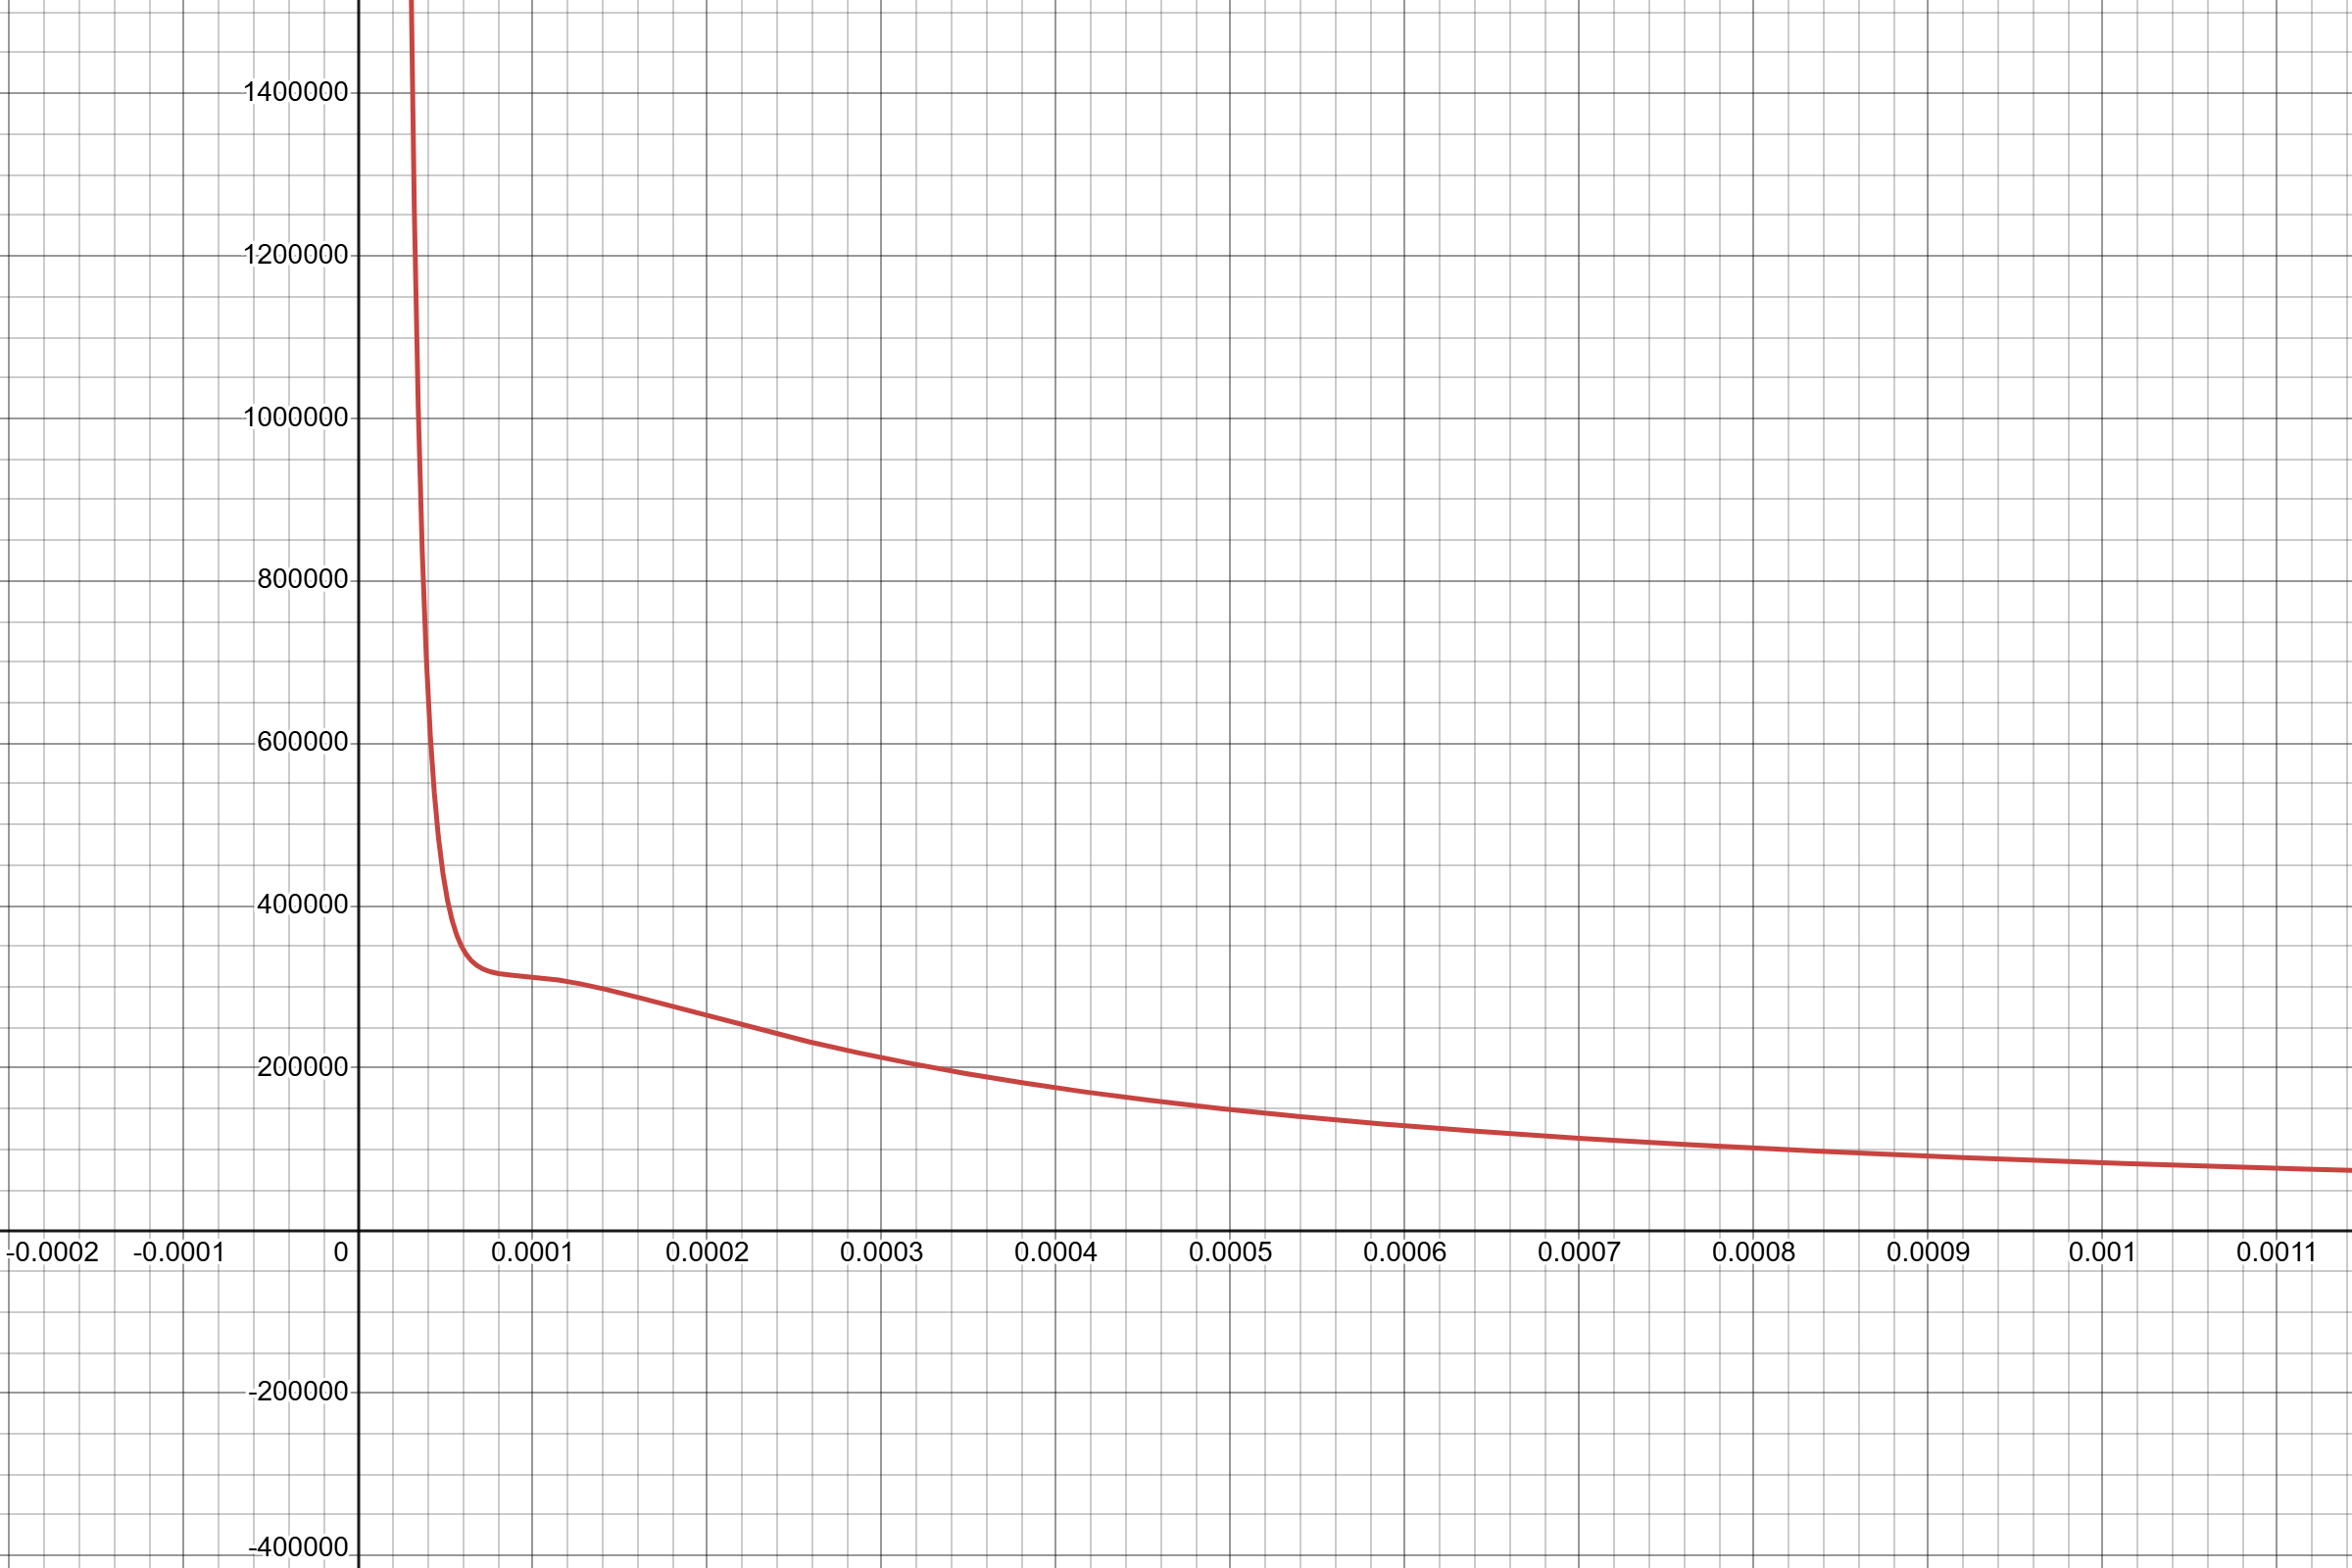
\includegraphics[width=\linewidth]{Graphics/Clausius/11_3.png}
        \caption{\label{fig:clausius_1}График 1. $P-V$ график уравнения Клаузиуса, $T = 11.3 \ \text{K}$}
    \end{minipage}
    \hfill
    \begin{minipage}{0.49\textwidth}
        \centering
        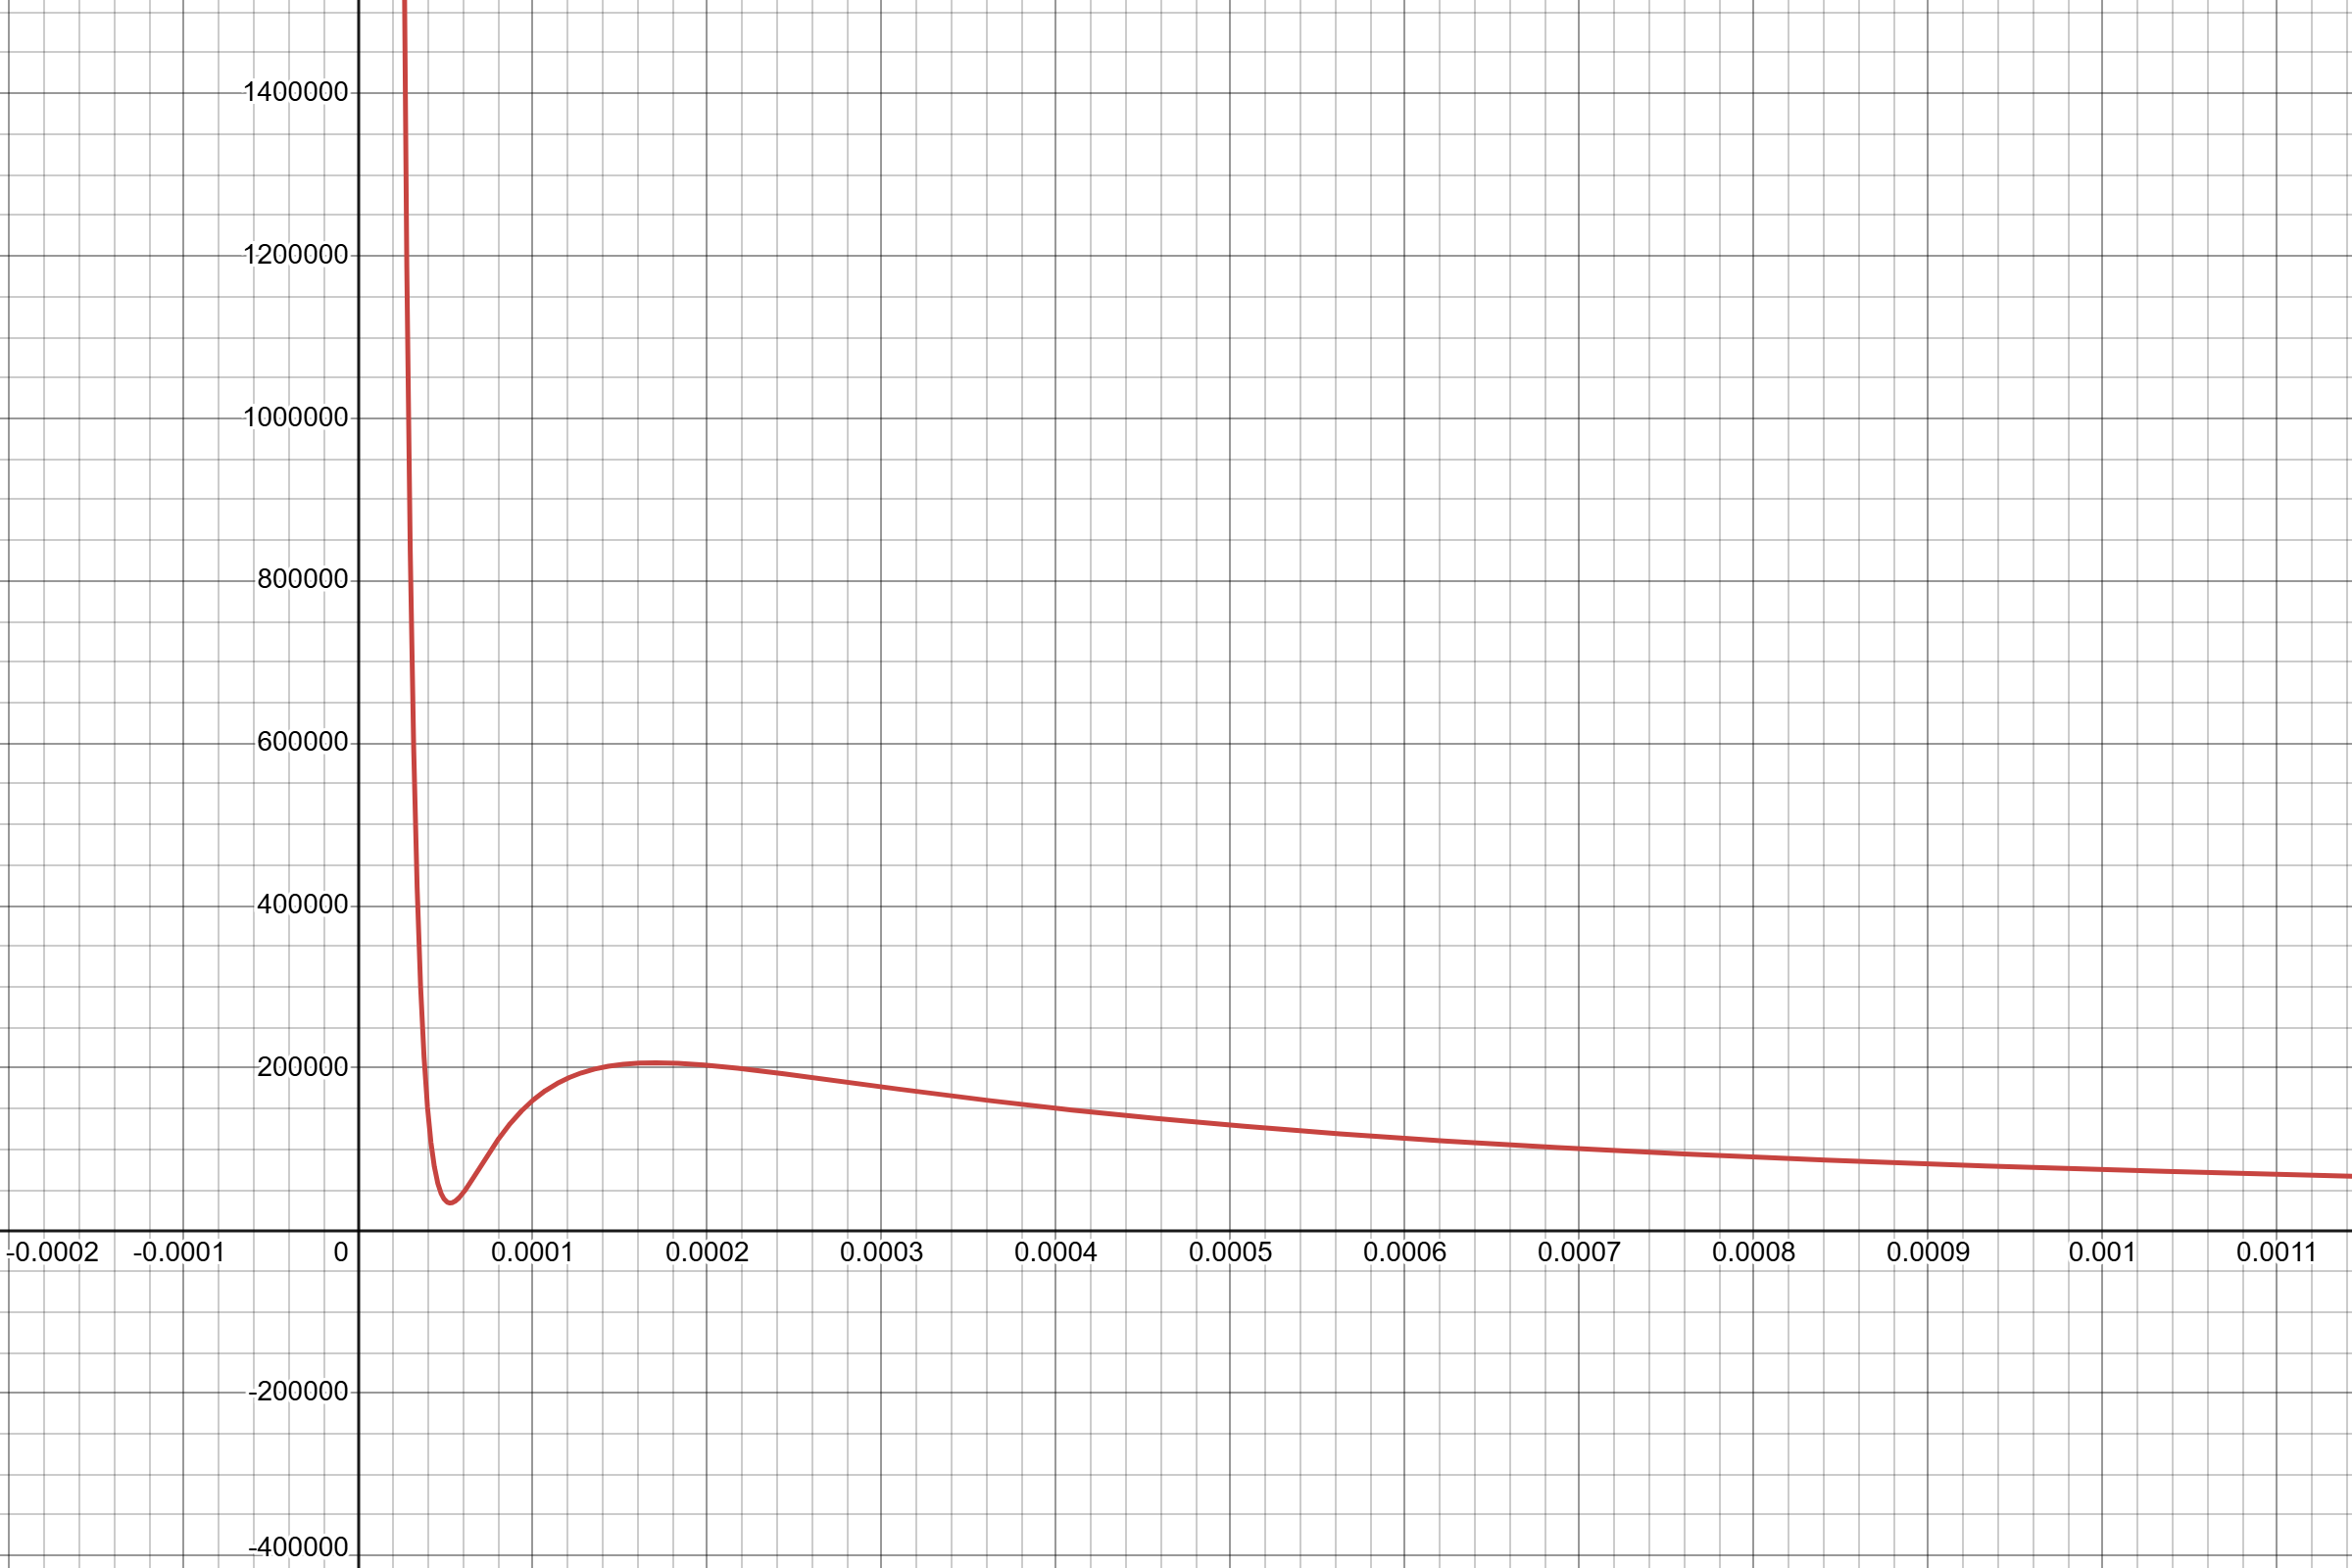
\includegraphics[width=\linewidth]{Graphics/Clausius/10_4.png}
        \caption{\label{fig:clausius_2}График 2. $P-V$ график уравнения Клаузиуса, $T = 10.4 \ \text{K}$}
    \end{minipage}
\end{figure}
Как мы видим, такой способ задания совсем не описывает реальные параметры азота. Данное уравнение плохо описывает фазовые переходы веществ.

\subsection{Уравнение Бертло}
В 1899 году Даниэль Бертло предложил упрощенную версию уравнения Клаузиуса.
\begin{equation}
      (P + \frac{a}{TV^2})(V - b) = RT,
\tag{\thesubsection}
\end{equation}
Оно также устарело, однако часто использовалось, поскольку рассчеты с ним были намного проще и точность была удовлетворительная. Критические параметры такие же, как у Клаузиуса при $c = 0$.

\subsection{Уравнение Дитеричи}
В 1899 году немецкий физик Конрад Дитеричи представил другой метод введения поправки на силы притяжения между молекулами. Это привело к уравнению вида:
\begin{equation}
      P = \frac{RT}{V-b}exp\left( -\frac{a}{RTV}\right).
\tag{\thesubsection}
\end{equation}
Уравнение Дитеричи хорошо подходит для описания плотных газов и жидкостей (учитывает экспоненциальное влияение сил притяжения между молекулами), однако плохо подходит для полярных или сильновзаимодействующих молекул.
Критические параметры:\\
- $V_c = 2b$,\\
- $T_c = \frac{a}{4bR}$,\\
- $P_c = \frac{a}{4e^2b^2R}$,\\
- $a = 2RV_cT_c = e^2V_c^2P_c$.\\
- $Z_c = \frac{1}{2e^2} \approx 0.2707$,\\
Построим график $P-V$ для азота.\\
Ссылка на построение в Desmos (дата обращения 18.06.2025): \href{https://www.desmos.com/calculator/ivahyshhxf}{https://www.desmos.com/calculator/ivahyshhxf}
\clearpage
\begin{figure}[h!]
    \centering
    \begin{minipage}{0.49\textwidth}
        \centering
        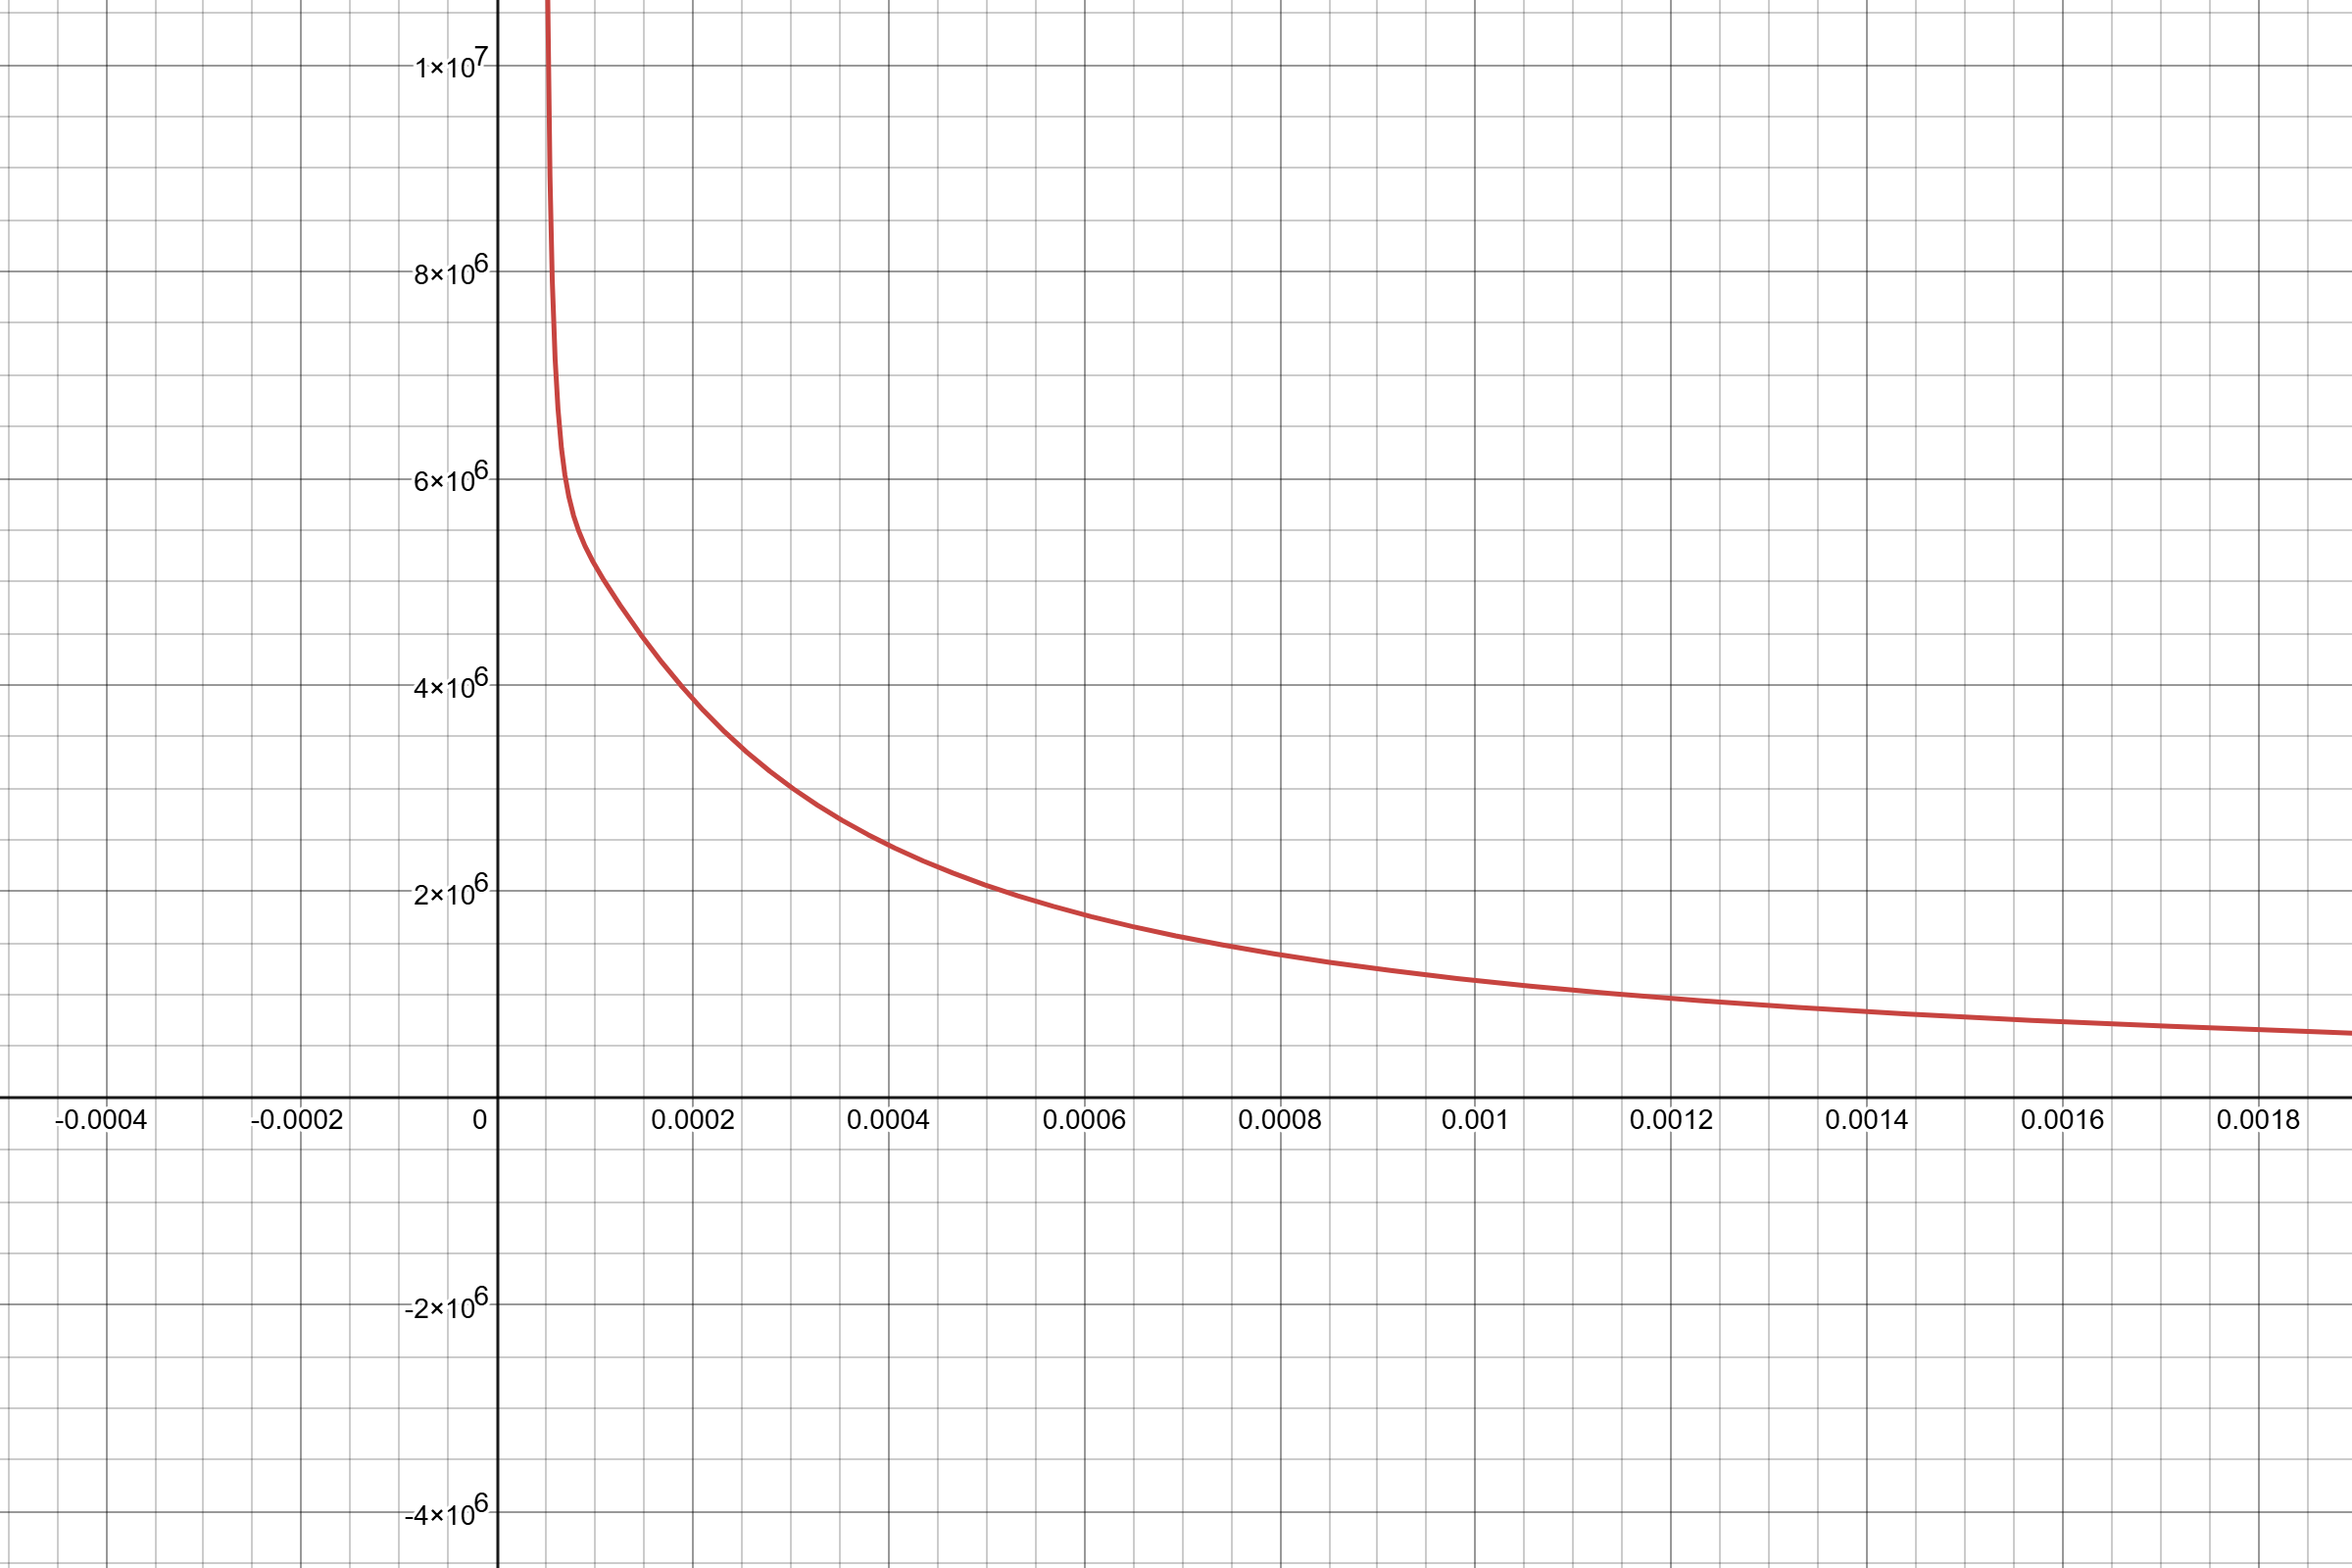
\includegraphics[width=\linewidth]{Graphics/Dieterici/152.png}
        \caption{\label{fig:clausius_1}График 3. $P-V$ график уравнения Дитеричи, $T = 152 \ \text{K}$}
    \end{minipage}
    \hfill
    \begin{minipage}{0.49\textwidth}
        \centering
        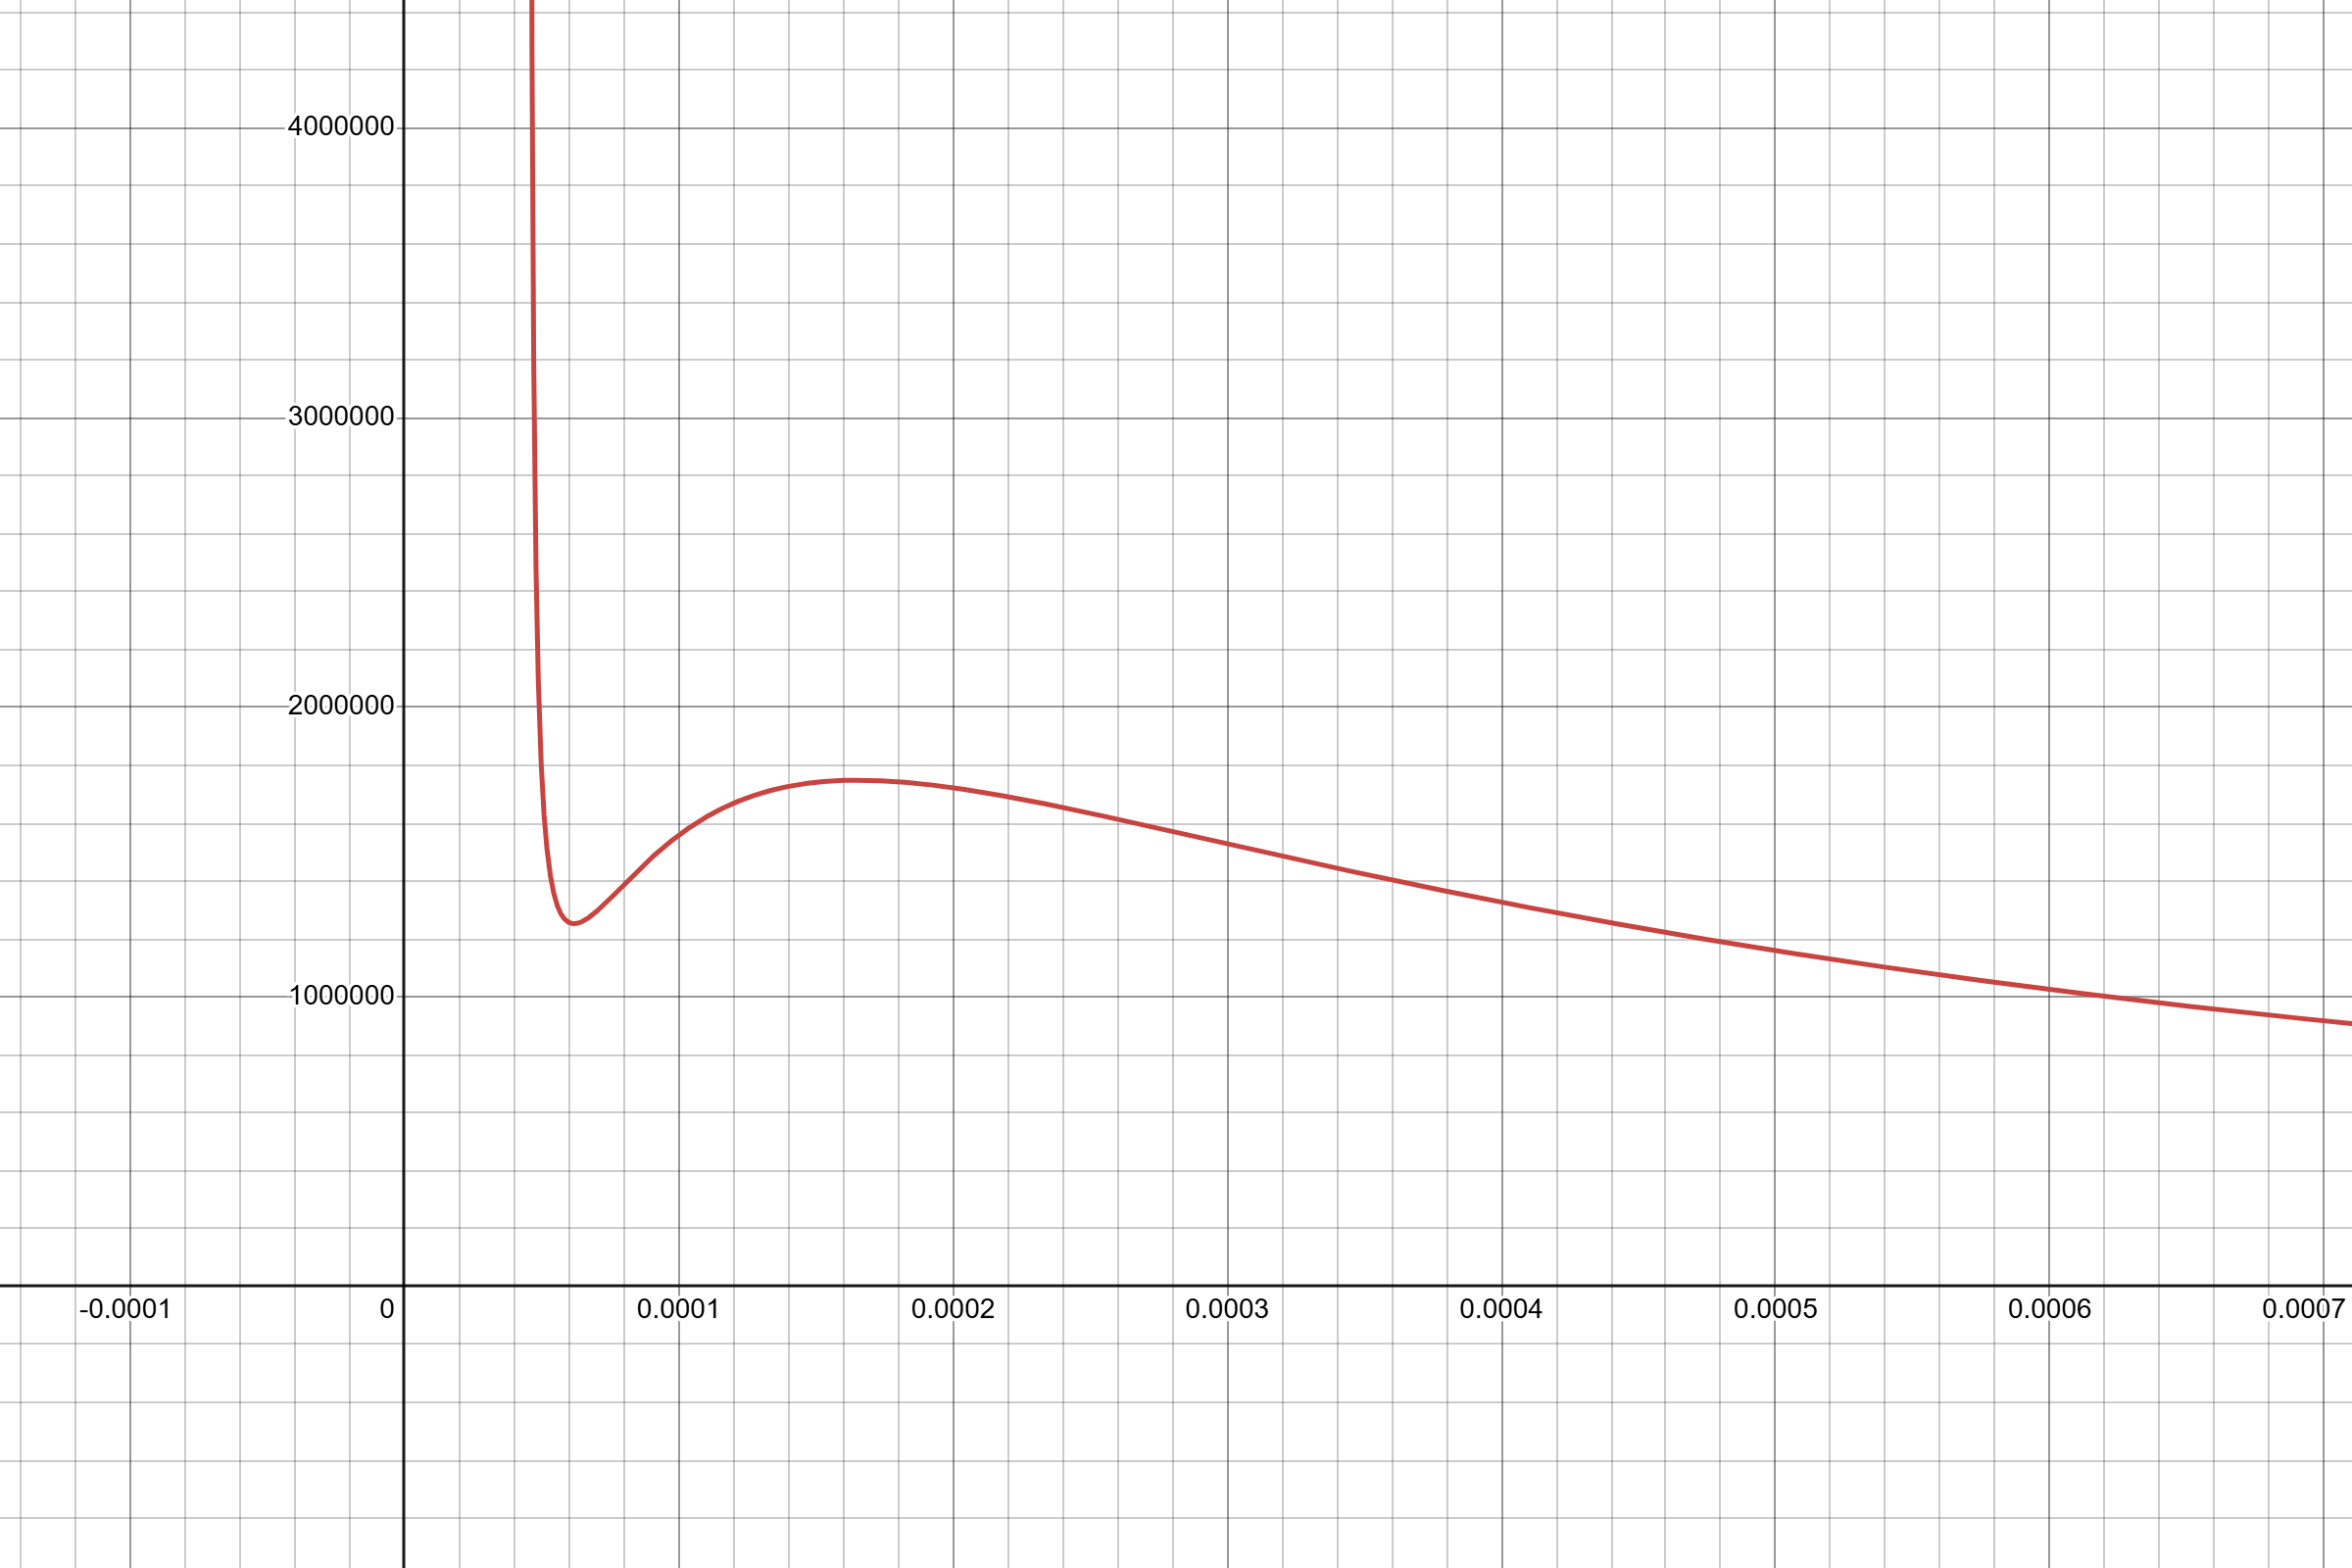
\includegraphics[width=\linewidth]{Graphics/Dieterici/100.png}
        \caption{\label{fig:clausius_2}График 4. $P-V$ график уравнения Дитеричи, $T = 100 \ \text{K}$}
    \end{minipage}
\end{figure}
\begin{figure}[h!]
    \centering
        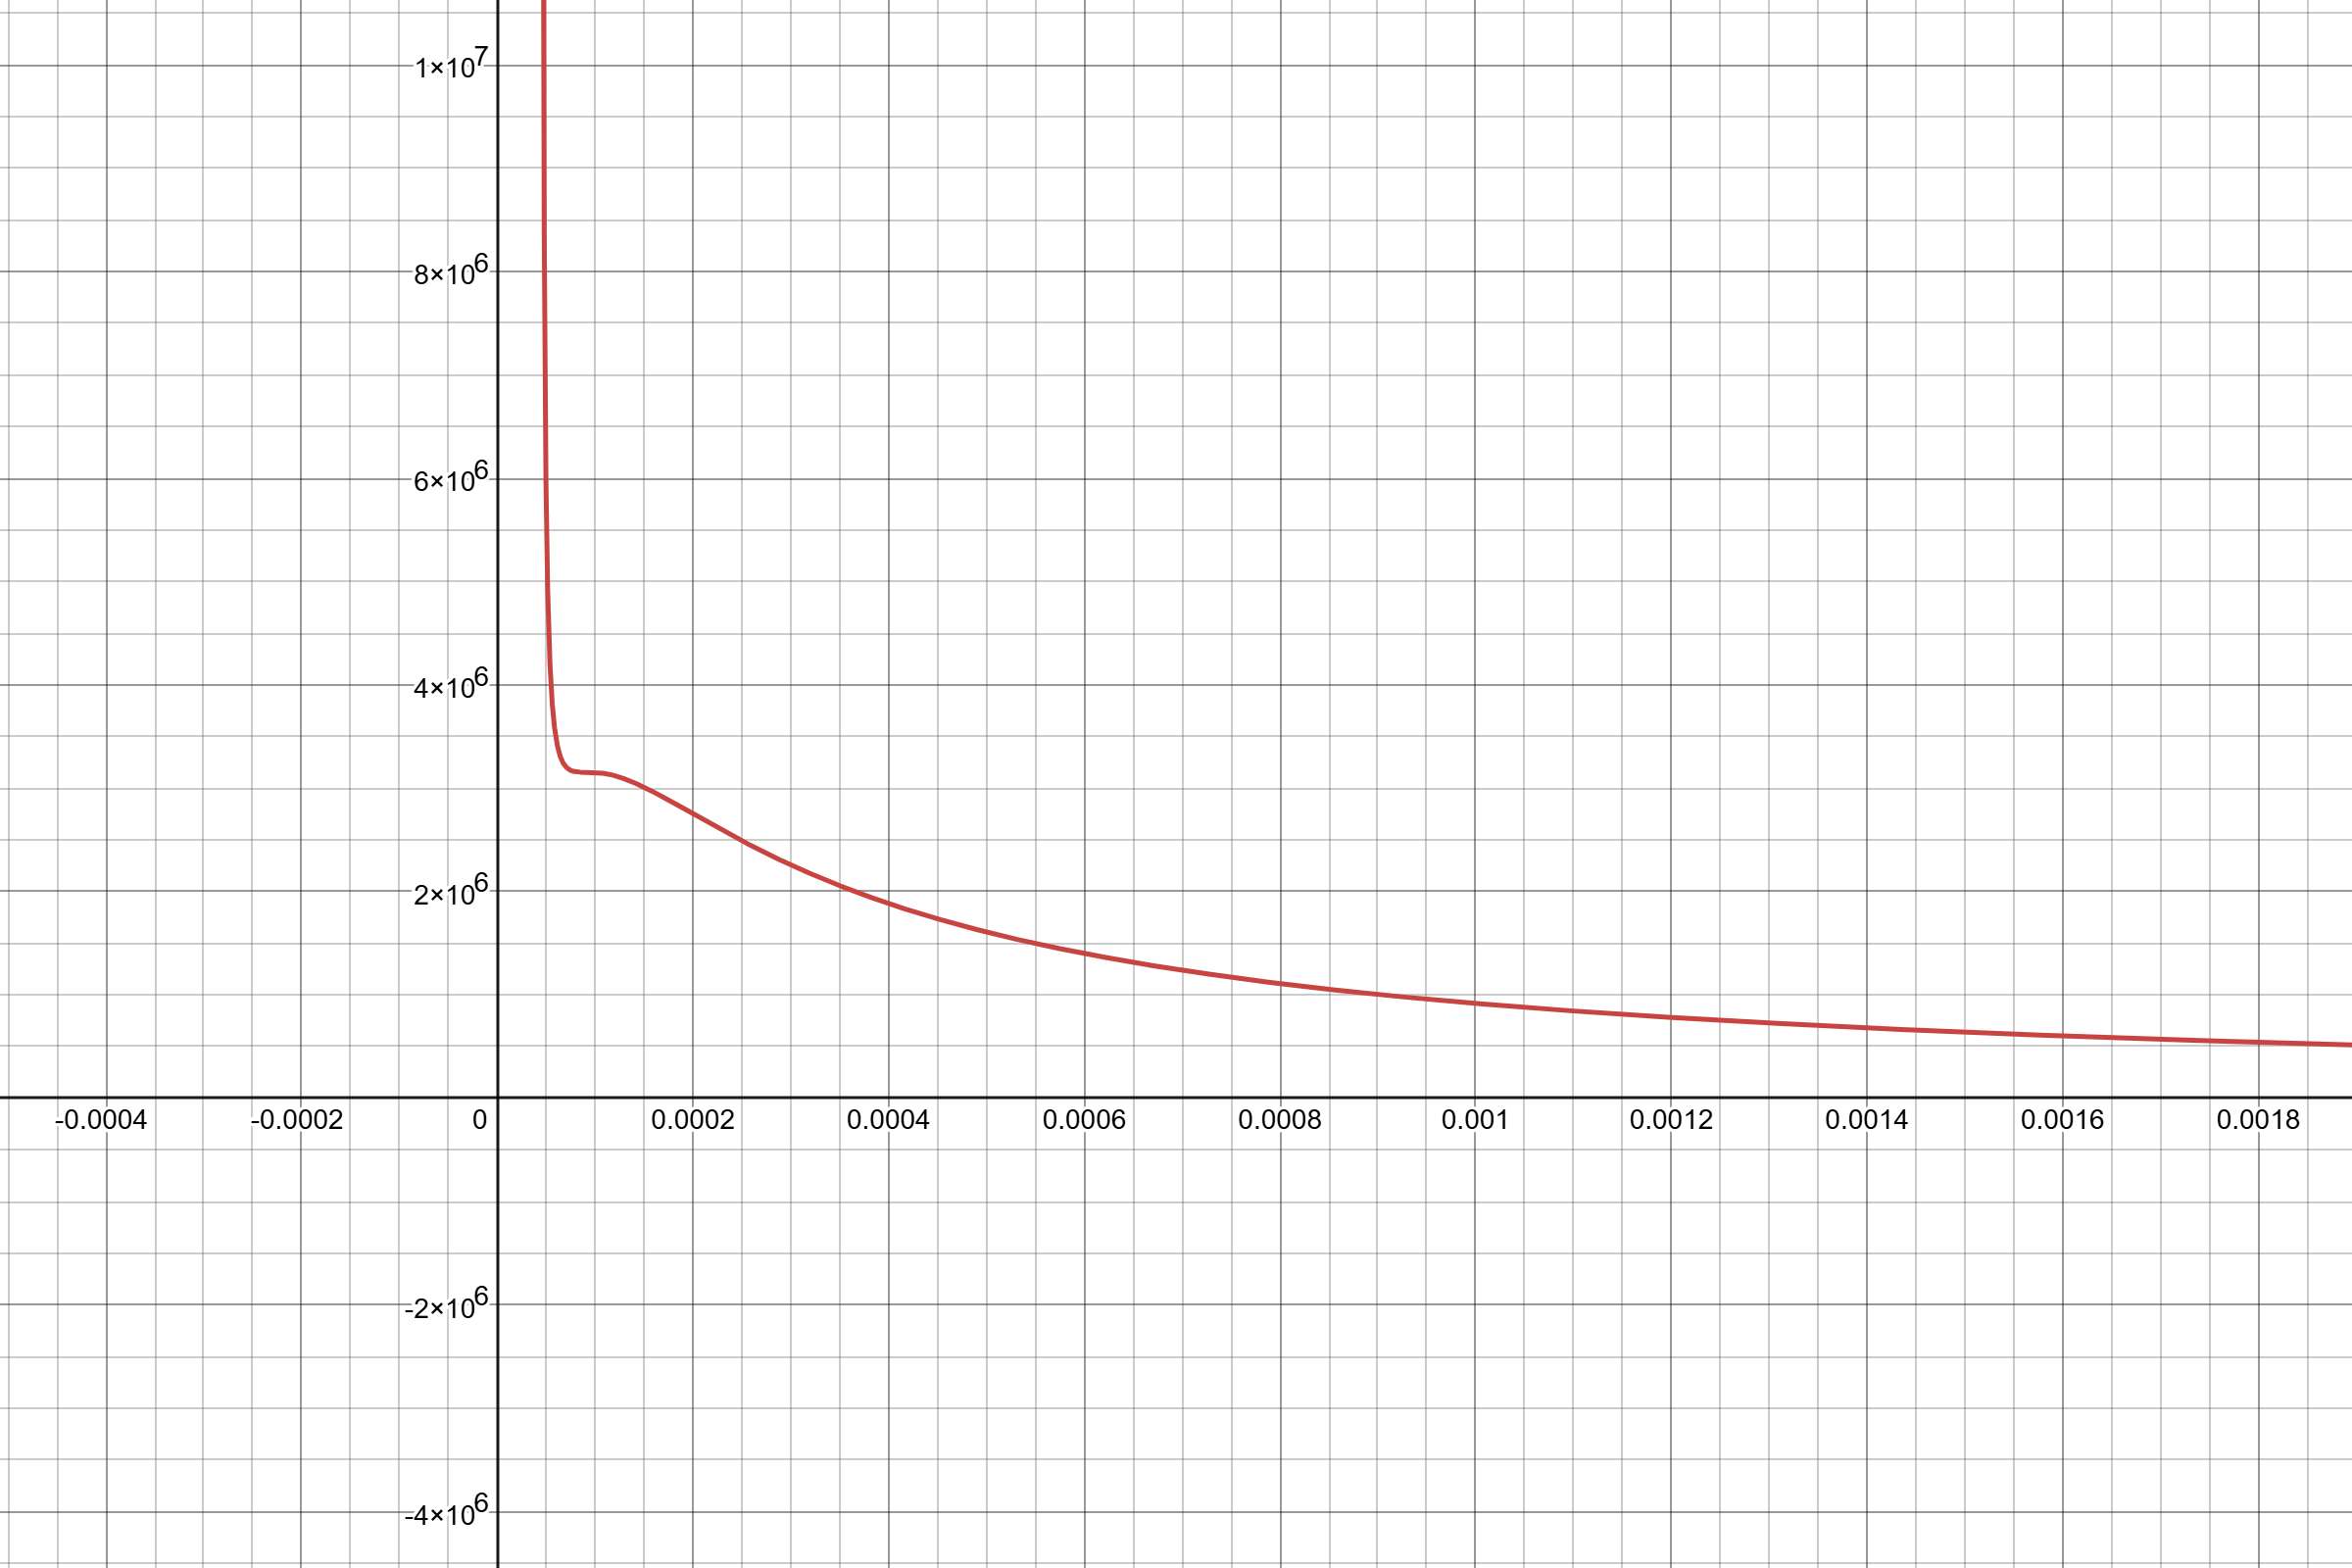
\includegraphics[width=\linewidth]{Graphics/Dieterici/126_21.png}
        \caption{\label{fig:clausius_1}График 5. $P-V$ график уравнения Дитеричи, $T = 126.21 \ \text{K}$}
\end{figure}
Как мы видим, уравнение Дитеричи с хорошей точностью описывает критическую точку.

\subsection{Вириальное уравнение}
В современном виде вириальное уравнение было развито в начале XX века. Общий вид:
\begin{equation}
      P = \frac{RT}{V}(1 + \frac{B(T)}{V} + \frac{C(T)}{V^2} + \frac{D(T)}{V^3} + . . .),
\tag{\thesubsection}
\end{equation}
где $B(T)$, $C(T)$, $D(T)$, ... - вириальные коэффициенты , зависящие от температуры.
Физический смысл коэффициентов 
\begin{itemize}
\item а) Второй вириальный коэффициент $B(T)$:\\
отвечает за вклад попарных взаимодействий между молекулами (силы притяжения и отталкивания)
\begin{equation*}
      B(T) = -2\pi N_A \displaystyle \int_0^{\inf} \ (e^{-\frac{U(r)}{kT}} - 1)r^2\ dr,
\end{equation*}
где $U(r)$ - потенциал межмолекулярного взаимодействия. Например, для потенциала Леннард-Джонса $U(r) = 4 \epsilon \left [ \left( \frac{\sigma}{r}\right )^{12} - \left( \frac{\sigma}{r}\right )^{6} \right ]$, $B(T)$ зависит от $\epsilon$ (глубина потенциальной ямы, максимальное притяжение) и от $\sigma$ (эффектимный диаметр частицы).
\item а) Третий вириальный коэффициент $C(T)$:\\
отвечает за вклад тройных столкновений (взаимодействие трёх молекул одновременно). Учитывает, что присутствие третьей молекулы изменяет парное взаимодействие двух других. Важно учитывать при высоких давлениях, т.к. вероятность тройных столкновений растёт.
\begin{equation*}
      C(T) = -\frac{8}{3}\pi^2 N_A^2 \displaystyle \int_0^{\infty} \displaystyle \int_0^{\infty} \ \left(e^{-\frac{U_3(r_{12}, r_{13}, r_{23})}{kT}} - e^{-\frac{U_2(r_{12}) + U_2(r_{13}) + U_2(r_{23})}{kT}}\right)r_{12}^2r_{13}^2\ dr_{12} dr_{13},
\end{equation*}
\item а) Четвертый и высшие коэффициенты ($D(T)$, ...):\\
Описывают более сложные взаимодействия, на практике используются только при очень высоких плотностях. 

Положительные значения коэффициентов говорят о доминировании сил отталкивания, отрицательные - сил притяжения. (Значения вторых коэффициентов для некоторых газов см. в приложении)
\end{itemize}
Данная модель хорошо теоретически обоснована и подходит для исследования разреженных газов с высокой точностью. Однако при больших давлениях ряд расходится и не подходит для сложных молекул. Модель довольно сложная из-за большого количества параметров. Построение данной модели есть в разделе 4, однако на графиках оно скрыто из-за сильной неточности, т.к. в доступе были только разложения до второго вириального коэффициента.

\subsection{Уравнение Битти-Бриджмена}
В 1927 году Джеймс Битти и Оскар Бриджмен опубликовали новое уравнение состояния вещества:
\begin{equation}
P = RT\frac{(1 - \epsilon)(V + B)}{V^2} - \frac{A}{V^2},
\tag{\thesubsection}
\end{equation}
где:\\
- $A = A_0\left(1 - \frac{a}{V}\right)$,\\
- $B = B_0\left(1 - \frac{b}{V}\right)$,\\
- $\epsilon = \frac{c}{VT^3}$,\\
- $A_0$, $B_0$, $a$, $b$, $c$ -- эмпирические постоянные.\\
Для данного уравнения выражение постоянных через критические параметры и наоборот не является аналитически простой задачей, как и нахождение $Z_c$.
В свойе статье они описывают физическое обоснование и применение (конспект физического обоснования из оригинальной статьи в приложении). Данное уравнение также подходит для правила смешивания (подробнее разбирается в уравнении SRK), однако точность сильно зависит от бинарных коэффициентов взаимодействия. Одно из самых точных эмперических уравнений состояния при давлениях меньше 200 атм. Учитывает температурную зависимость сил межмолекулярного взаимодействия.

\subsection{Уравнение Редлиха-Квонга}
В 1949 году Отто Редлих и Джозеф Квонг предложили для описания состояния газов уравнение, далее (RK - уравнение состояния Redlich-Kwong):
\begin{equation}
      P = \frac{RT}{V-b} - \frac{a}{\sqrt{T}V(V+b)}.
\tag{\thesubsection}
\end{equation}

Числитель первого слагаемого $(V-b)$ остался из уравнения Ван-дер-Ваальса, а числитель второго $V(V+b)$ имеет примерно такое же обоснование, что у Класузиуса. Основные отличия:\\
а) форма $V(V+b)$ лучше отражает асимметрию потенциала взаимодействия. При $V \gg b$: $V(V+b) \approx V^2$ (как у Ван-дер-Ваальса), при $V \rightarrow b$: $V(V+b) \approx 2b^2$, что предотвращает слишком резкий рост давления (в отличие от уравнения Клаузиуса, где ($(V+c)^2 \approx 4b^2$). Форма дает асимптотику более близкую к экспериментальной.\\
б) Лучше согласовывается с вириальным разложением
\begin{equation*}
      \frac{PV}{RT} = 1 + \frac{B(T)}{V} + \frac{C(T)}{V^2} + . . .
\end{equation*}
Если разложить RK, получим:
\begin{equation*}
      \frac{PV}{RT} = 1 + \left( b - \frac{a}{RT^{3/2}}\right)\frac{1}{V} + \left( b^2 - \frac{ab}{RT^{3/2}}\right)\frac{1}{V^2} + . . .
\end{equation*}
Отсюда $B(T) = b - \frac{a}{RT^{3/2}}$. Разложим теперь уравнение Клаузиуса:
\begin{equation*}
      \frac{PV}{RT} = 1 + \left( b - \frac{a}{RT^{2}}\right)\frac{1}{V} + \left( b^2 - \frac{2aс}{RT^{2}}\right)\frac{1}{V^2} + . . .
\end{equation*}
Отсюда $B(T) = b - \frac{a}{RT^{2}}$. Эксперименты показывают, что зависимость $B(T) \sim \frac{1}{T^2}$ слишком сильная, поэтому модель Редлиха-Квонга лучше описывает поведение газа.\\
в) Найдем связь критических параметров с коэффициентами и критическую сжимаемость.
$$
\begin{cases}
\left( \frac{\partial P}{\partial V} \right)_{T=T_c} = 0,\\[10pt]
\left( \frac{\partial^2 P}{\partial V^2} \right)_{T=T_c} = 0.
\end{cases}
\begin{cases}
-\frac{R T_c}{b^2 (V - 1)^2} + \frac{a}{\sqrt{T_c}} \left( \frac{2V + b}{V^2 (V + b)^2} \right) = 0,\\[10pt]
\frac{2 R T_c}{ (V - b)^3} - \frac{2a}{\sqrt{T_c}} \left( \frac{3V^2 + 3bV + b^2}{V^3 (V + 1)^3}\right) = 0. 
\end{cases}
$$
\begin{equation*}
\frac{1}{V-b} = \frac{3V^2 + 3bV + b^2}{V(V+b)(2V+b)}
\end{equation*}
\begin{equation*}
V_c = 2^{\frac{2}{3}}b + 2^{\frac{1}{3}}b + b \approx \frac{b}{2^{\frac{1}{3}} - 1} \approx 3.8473 \cdot b.
\end{equation*}
Для точности обозначим за $\alpha = 2^{\frac{2}{3}} + 2^{\frac{1}{3}} + 1$.
Подставив в первое уравнение системы $V$, получим соотношение $a = bRT^{\frac{3}{2}}\frac{\alpha^2(\alpha+1)^2}{(\alpha-1)^2(2\alpha+1)}$Подставим в уравнение состояния и выразим коэффициент $b$.
\begin{equation*}
	b = \frac{RT_c}{P_c}\frac{\alpha^2-2\alpha-1}{(\alpha-1)^2(2\alpha+1)} \approx 0.08664\frac{RT_c}{P_c},
\end{equation*}
\begin{equation*}
	a = \frac{R^2T_c^{\frac{5}{2}}}{P_c}\frac{\alpha^2(\alpha+1)^2(\alpha^2-2\alpha-1)}{(\alpha-1)^4(2\alpha+1)^2} \approx 0.42748\frac{R^2T_c^{\frac{5}{2}}}{P_c},
\end{equation*}
\begin{equation*}
	T_c = \frac{a^{\frac{2}{3}}}{0.42748 \cdot R^{\frac{2}{3}}b^{\frac{2}{3}}},
\end{equation*}
\begin{equation*}
	P_c = \frac{a^{\frac{2}{3}}}{0.08664 \cdot R^{\frac{1}{3}}b^{\frac{5}{3}}},
\end{equation*}
\begin{equation*}
	Z_c = \frac{P_cV_c}{RT_c} = \frac{\alpha bP_c}{RT_c} = \frac{\alpha^3-2\alpha^2-\alpha}{2\alpha^3-3\alpha^2+1} = \frac{1}{3} \approx 0.333,
\end{equation*}
Таким образом, мы получили, что значение критической сжимаемости, которое дает уравнение Редлиха-Квонга для всех газов, довольно близко к реальным значениям (уравнение Ван-дер-Ваальса дает $Z_c = \frac{3}{8} = 0.375$).
Сами Редлих и Квонг утверждают, что зависимость $\frac{a}{\sqrt{T}V(V+b)} \sim \frac{1}{\sqrt{T}}$ подобрана эмперически и они не опирались на квантовую механику, связанную с зависимостью взаимодействия молекул от температуры. Поэтому данная модель плохо подходит для описания состояния полярных газов (где, как мы знаем, зависят ориентационные силы от температуры как $\sim \frac{1}{T}$) .
Данная модель улучшила асимптотику при высоких температурах, а также согласовала "зону действия" сил притяжения и отталкивания (к слову, у Клаузиуса параметры $b$ и $c$ не были согласованы).

\subsection{Уравнение Соаве-Редлиха-Квонга}
\renewcommand{\thefootnote}{*} 
В 1972 году итальянский ученый и инженер Джорджио Соаве внес модификацию в уравнение Редлиха-Квонга:
\begin{equation}
      P = \frac{RT}{V-b} - \frac{a(T)}{V(V+b)},
\tag{\thesubsection}
\end{equation}
где:\\
- $a(T) = a_0 \cdot \alpha(T)$,\\
- $\alpha(T) = \left[ 1 + \kappa(1-\sqrt{\frac{T}{T_c}})\right]^2$,\\
- $\kappa = 0.48508 + 1.55171\omega - 0.15613\omega^2$,\\
- $a_0 = 0.42748\frac{R^2T_c^{2}}{P_c}$ (как в RK),\\
- $b = 0.08664\frac{RT_c}{P_c}$ (как в RK).\\
- $\omega$ - ацентрический фактор\footnotemark{},\\
Критические параметры такие же, как в RK.
Соаве сделал зависимость межмолекулярных сил от температуры более более гибкой. Теперь в уравнении используется ацентрический фактор $\omega$ - концептуальное число, которое ввел Кеннет Питцер в 1955 году. Его также называют мерой несферичности молекулы. Питцер определил $\omega$ из соотношения
\begin{equation}
     \omega = -log_{10}(p^{sat}_r) - 1 \text{ при } T_r = 0.7,
\end{equation}
где:
- $p^{sat}_r = \frac{p^{sat}}{p_c}$ -- пониженное давление насыщенных паров,\\
- $T_r = \frac{T}{T_c}$ -- пониженнае температура. \\
Для гелия ацентрический фактор равен -0.388; аргона, криптона и ксенона 0.000, а для молекулы воды 0.343, а для 1,2-Пропилен гликоля 1.102. Чем больше ацентричесий фактор, тем тем ниже давление насыщенного пара (хуже испаряются), значит молекулы сильнее притягиваются. Гелий легко испаряется (низки ацентричесий фактор), а более длинные цепочки и сильные водородные связи обеспечивают сильное притяжение из-за вандерваальсовых сил. Некоторые ацентричесие факторы представлены в приложении.\\
\footnotetext{Подробнее об этом можно прочитать в J.M. Smith, Hendrick Van Ness, Michael Abbott, Mark Swihart - Introduction to Chemical Engineering Thermodynamics-McGraw-Hill Education (2018), где также ссылаются на оригинальный труд Питцера}
\renewcommand{\thefootnote}{\arabic{footnote}} 
Модификация Соаве сделало уравнение состояния RK универсальным для широкого класса веещств: от простых газов, до тяжелых углеродов. А также улучшила точность при расчете давления насыщеного пара. Более того, теперь стало возможным с хорошей точностью рассчитывать равнение состояние смеси газов. Для смесей можно использовать простые правила смешивания: 
\begin{align}
     \displaystyle a_{\text{смеси}} &= \sum_i \sum_j x_ix_j(a_ia_j)^{\frac{1}{2}}(1-k_{ij}), & b_{\text{смеси}} &= \sum_i x_ib_i,
\end{align}
где:\\
- $x_i$, $x_j$ -- молярные доли компонентов смеси,\\
- $a_i$, $a_j$ -- параметры притяжения чистых веществ,\\
- $b_i$ -- параметр объема чистого вещества,
- $k_{ij}$ -- бинарный коэффициент взаимодействия Он показывает, насколько взаимодействие между компонентами i и j отличается от среднего значения $(a_ia_j)^{\frac{1}{2}}$. Обычно его определяют экспериментально или берут из баз данных. Некоторые приведены в приложении.

\subsection{Уравнение Пенга–Робинсона} 
Уравнение стостояния Пенга-Робинсона (PR) было разработано в 1976 году Дин-Ю Пенгом и Дональдом Робинсоном.
\begin{equation}
      P = \frac{RT}{V-b} - \frac{a(T)}{V(V+b) - b(V-b)},
\tag{\thesubsection}
\end{equation}
где:\\
- $a(T) = a_0 \cdot \alpha(T)$,\\
- $\alpha(T) = \left[ 1 + \kappa(1-\sqrt{\frac{T}{T_c}})\right]^2$,\\
- $\kappa = 0.37464 + 1.54226\omega - 0.26992\omega^2$,\\
- $\omega$ - ацентрический фактор,\\
- $a_0 = 0.45724\frac{R^2T_c^{2}}{P_c}$,\\
- $b = 0.07780\frac{RT_c}{P_c}$.\\
Проделав тот же алгоритм, получим, что:\\
- $V_c = \alpha b$, $\alpha = \frac{\sqrt[3]{4}}{\sqrt[3]{2-\sqrt{2}}} + \sqrt[3]{2}\sqrt[3]{2-\sqrt{2}} \approx 3.95137$,\\
- $T_c = \frac{a^{\frac{2}{3}}}{0.45724 \cdot R^{\frac{2}{3}}b^{\frac{2}{3}}}$, $P_c = \frac{a^{\frac{2}{3}}}{0.07780 \cdot R^{\frac{1}{3}}b^{\frac{5}{3}}}$,\\
- $Z_c \approx 0.3074$ (еще ближе к реальности).\\
Данная модель разрабатывалась для более точного описания жидкостей и сложных углеродных связей. Знаменатель $V(V+b) - b(V-b)$ отражает несимметричность молекул, а также данная поправка делает уравнение более чувствительным к изменению плотности. К примеру, пусть $V = 2b$, тогда в SRK $\delta_{SRK} = V(V+b) = 6b^2$, в PR $\delta_{PR} = V(V+b) - b(V-b) = 7b^2$. Это отражает, что при малых молярных объемах силы притяжения описываемые PR меньше, что лучше согласуется с поведением жикдостей и плотных газов. Также данная модель лучше описывает вещества, имеющие высокую полярность, водородные связи, высокое значение ацентрического фактора $\omega$, поэтому активно используется в нефтегазовой промышленности. 

\subsection{Современные уравнения состояния}
Сейчас основные современные модели -- это не просто кубические уравнения , а сложные функции, учитывающие молекулярное строение вещества.
\begin{enumerate}
\item SAFT (Statistical Associating Fluid Theory).\\
 Это статистико-термодинамическое уравнение , основанное на теории возмущений цепочечных молекул. Учитывает:
\begin{itemize}
\item водородные связи,
\item форму молекул,
\item полярность,
\item длинные углеводородные цепочки.
\end{itemize}
Применяется в нефтегазовых отраслях, проектировании химических растворов, включая электролиты.

\item GERG-2008 (German-Russian Equation of State).\\
Это многочленное уравнение , построенное на основе экспериментальных данных. Это аналитическое уравнение, и представляет собой разложение в ряд по плотности и температуре.\\
Применяется при расчете сжимаемости, взаимодействия газов под высоким давлением.

\item CPA (Cubic-Plus-Association)\\
Это модификация классического кубического уравнения (например, SRK), дополненная моделью ассоциации.
\begin{equation*}
P = P_{\text{кубическое}} + P_{\text{ассоциация}}.
\end{equation*}
Подходит для работы с водой, спиртами, кислотами, аминами.
\end{enumerate}

На данный момент насчитывает около 150-200 уравнений состояния, однако широко используется около 20-30. Это показывает, что подобрать уравнение, идеально описывающее все вещества при всех параметрах - невозможно. Также тяжело найти баланс между точностью и простотой использования.

\section{Сравнение некоторых уравнений}
В данном разделе предлагается пронаблюдать зависимость $P-V-T$ в координатах $P-V$ при некоторых $T$.\\
Обозначения:\\
- \textcolor{red}{красный} -- уравнение Менделеева-Клапейрона (идеальный газ),\\
- \textcolor{orange}{оранжевый} -- уравнение Ван-дер-Ваальса,\\
- \textcolor{green}{зеленый} -- уравнение Битти-Бриджмена,\\
- \textcolor{blue}{синий} -- уравнение Редлиха-Квонга,\\
- \textcolor{purple}{фиолетовый} -- уравнение Соаве-Редлиха-Квонга,\\
- \textbf{черный} -- уравнение Пенга-Робинсона,\\
- скрыто: \textcolor{red}{красный} пунктир -- вириальное уравнение.\\
В открытом можно найти коэффициенты для некоторых газов уравнения Битти-Бриджмена (в приложении они взяты из оригинальной статьи). Коэффициенты для уравнения Ван-дер-Ваальса были взяты из книги Лабораторный практикум по общей физике, Том I, Термодинамика и молекулярная физика. Критические температуры и давления взяты тоже оттуда, а объем из приложения. Все остальные необходимые параметры можно найти в приложении.\\
Экспериментальные коэффициенты для уравнений RK, SRK и PR найти не удалось в связи с тем, что бесплатных открытых источников практически нет (однако если читатель может их предоставить, то это бы сильно помогло). Поэтому мы пользовались формулами соотношений постоянных и критических параметров. 
Как мы дальше увидим, это приведет в случае PR к неточному построению.
Ссылка на построение в Desmos (дата обращения 18.06.2025): \\
- $N_2$: \href{https://www.desmos.com/calculator/mj5jolx1gp}{https://www.desmos.com/calculator/mj5jolx1gp},\\
- $CO_2$: \href{https://www.desmos.com/calculator/zkhsuoilkw}{https://www.desmos.com/calculator/zkhsuoilkw},\\
- $He$: \href{https://www.desmos.com/calculator/f8ht6qa0za}{https://www.desmos.com/calculator/f8ht6qa0za},\\
- $H_2O$: \href{https://www.desmos.com/calculator/2kdq2ihwje}{https://www.desmos.com/calculator/2kdq2ihwje},\\
- $H_2$: \href{https://www.desmos.com/calculator/ubchzwryms}{https://www.desmos.com/calculator/ubchzwryms},\\
- $O_2$: \href{https://www.desmos.com/calculator/xncelfhisb}{https://www.desmos.com/calculator/xncelfhisb},\\
\begin{figure}[h!]
    \centering
    \begin{minipage}{0.49\textwidth}
        \centering
        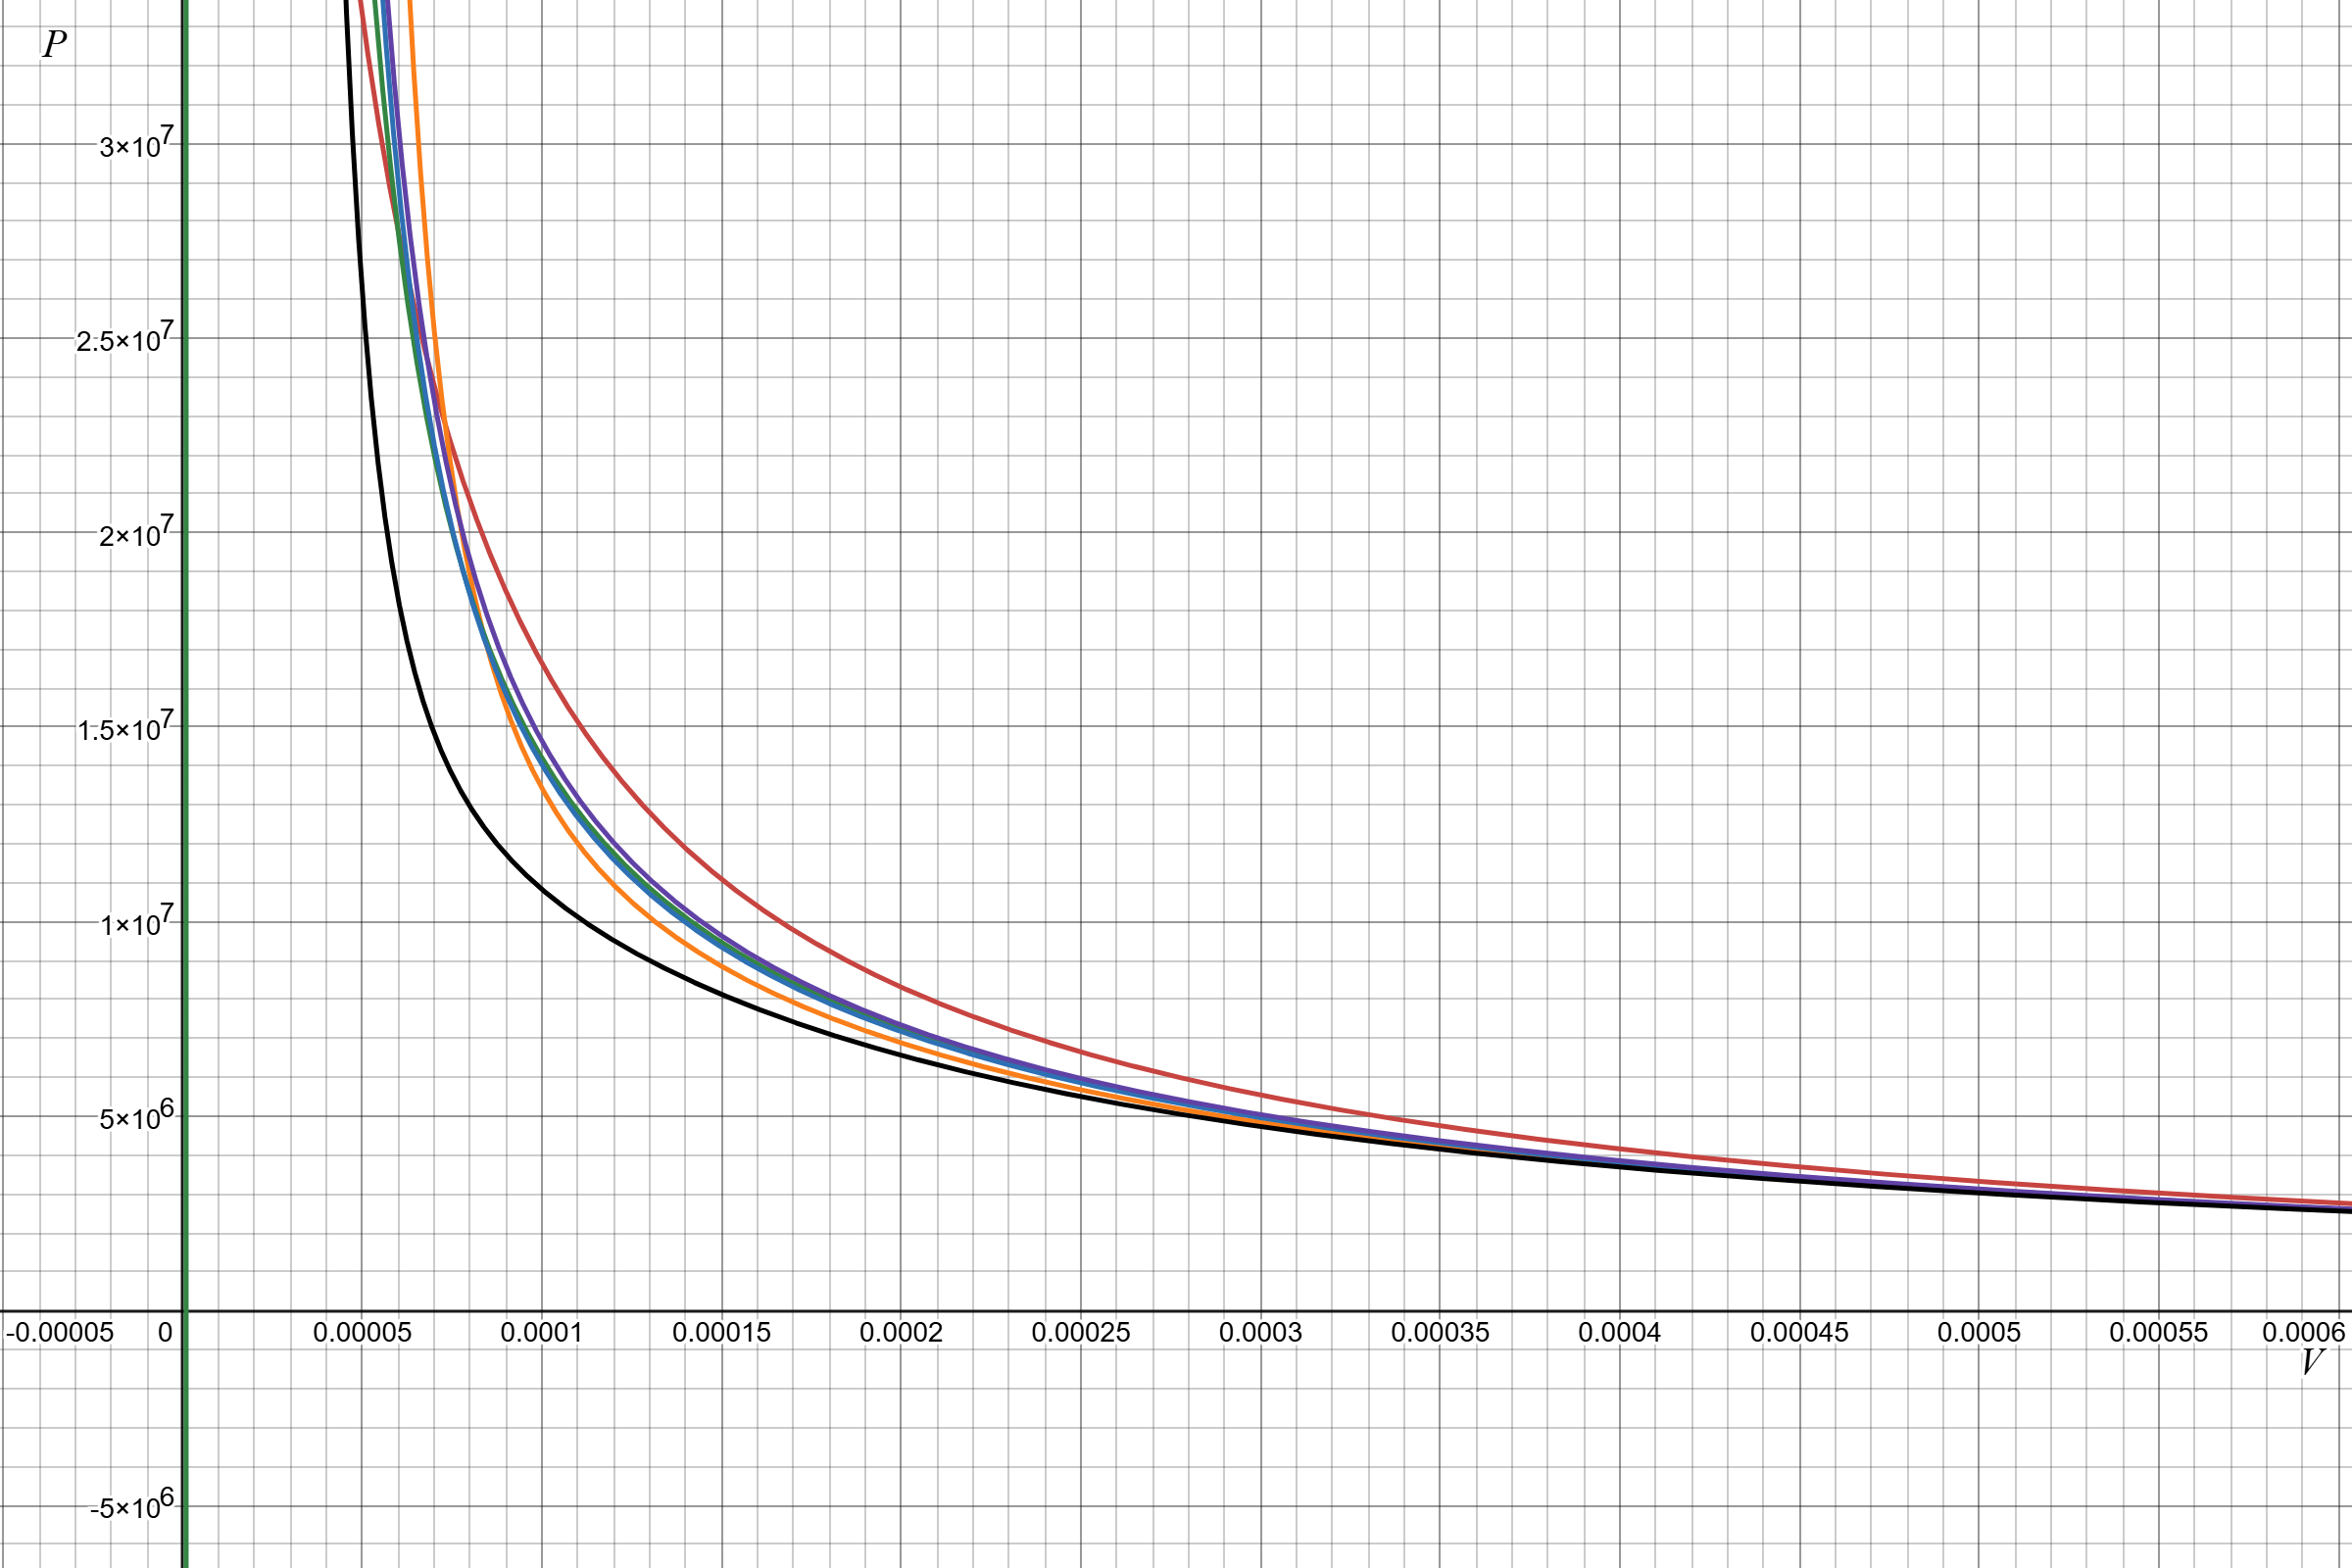
\includegraphics[width=\linewidth]{Graphics/N2/200.png}
        \caption{\label{fig:clausius_1}График 6. $P-V$ сравнительное построение графиков уравнений состояния азота $N_2$, $T = 200 \ \text{K}$}
    \end{minipage}
    \hfill
    \begin{minipage}{0.49\textwidth}
        \centering
        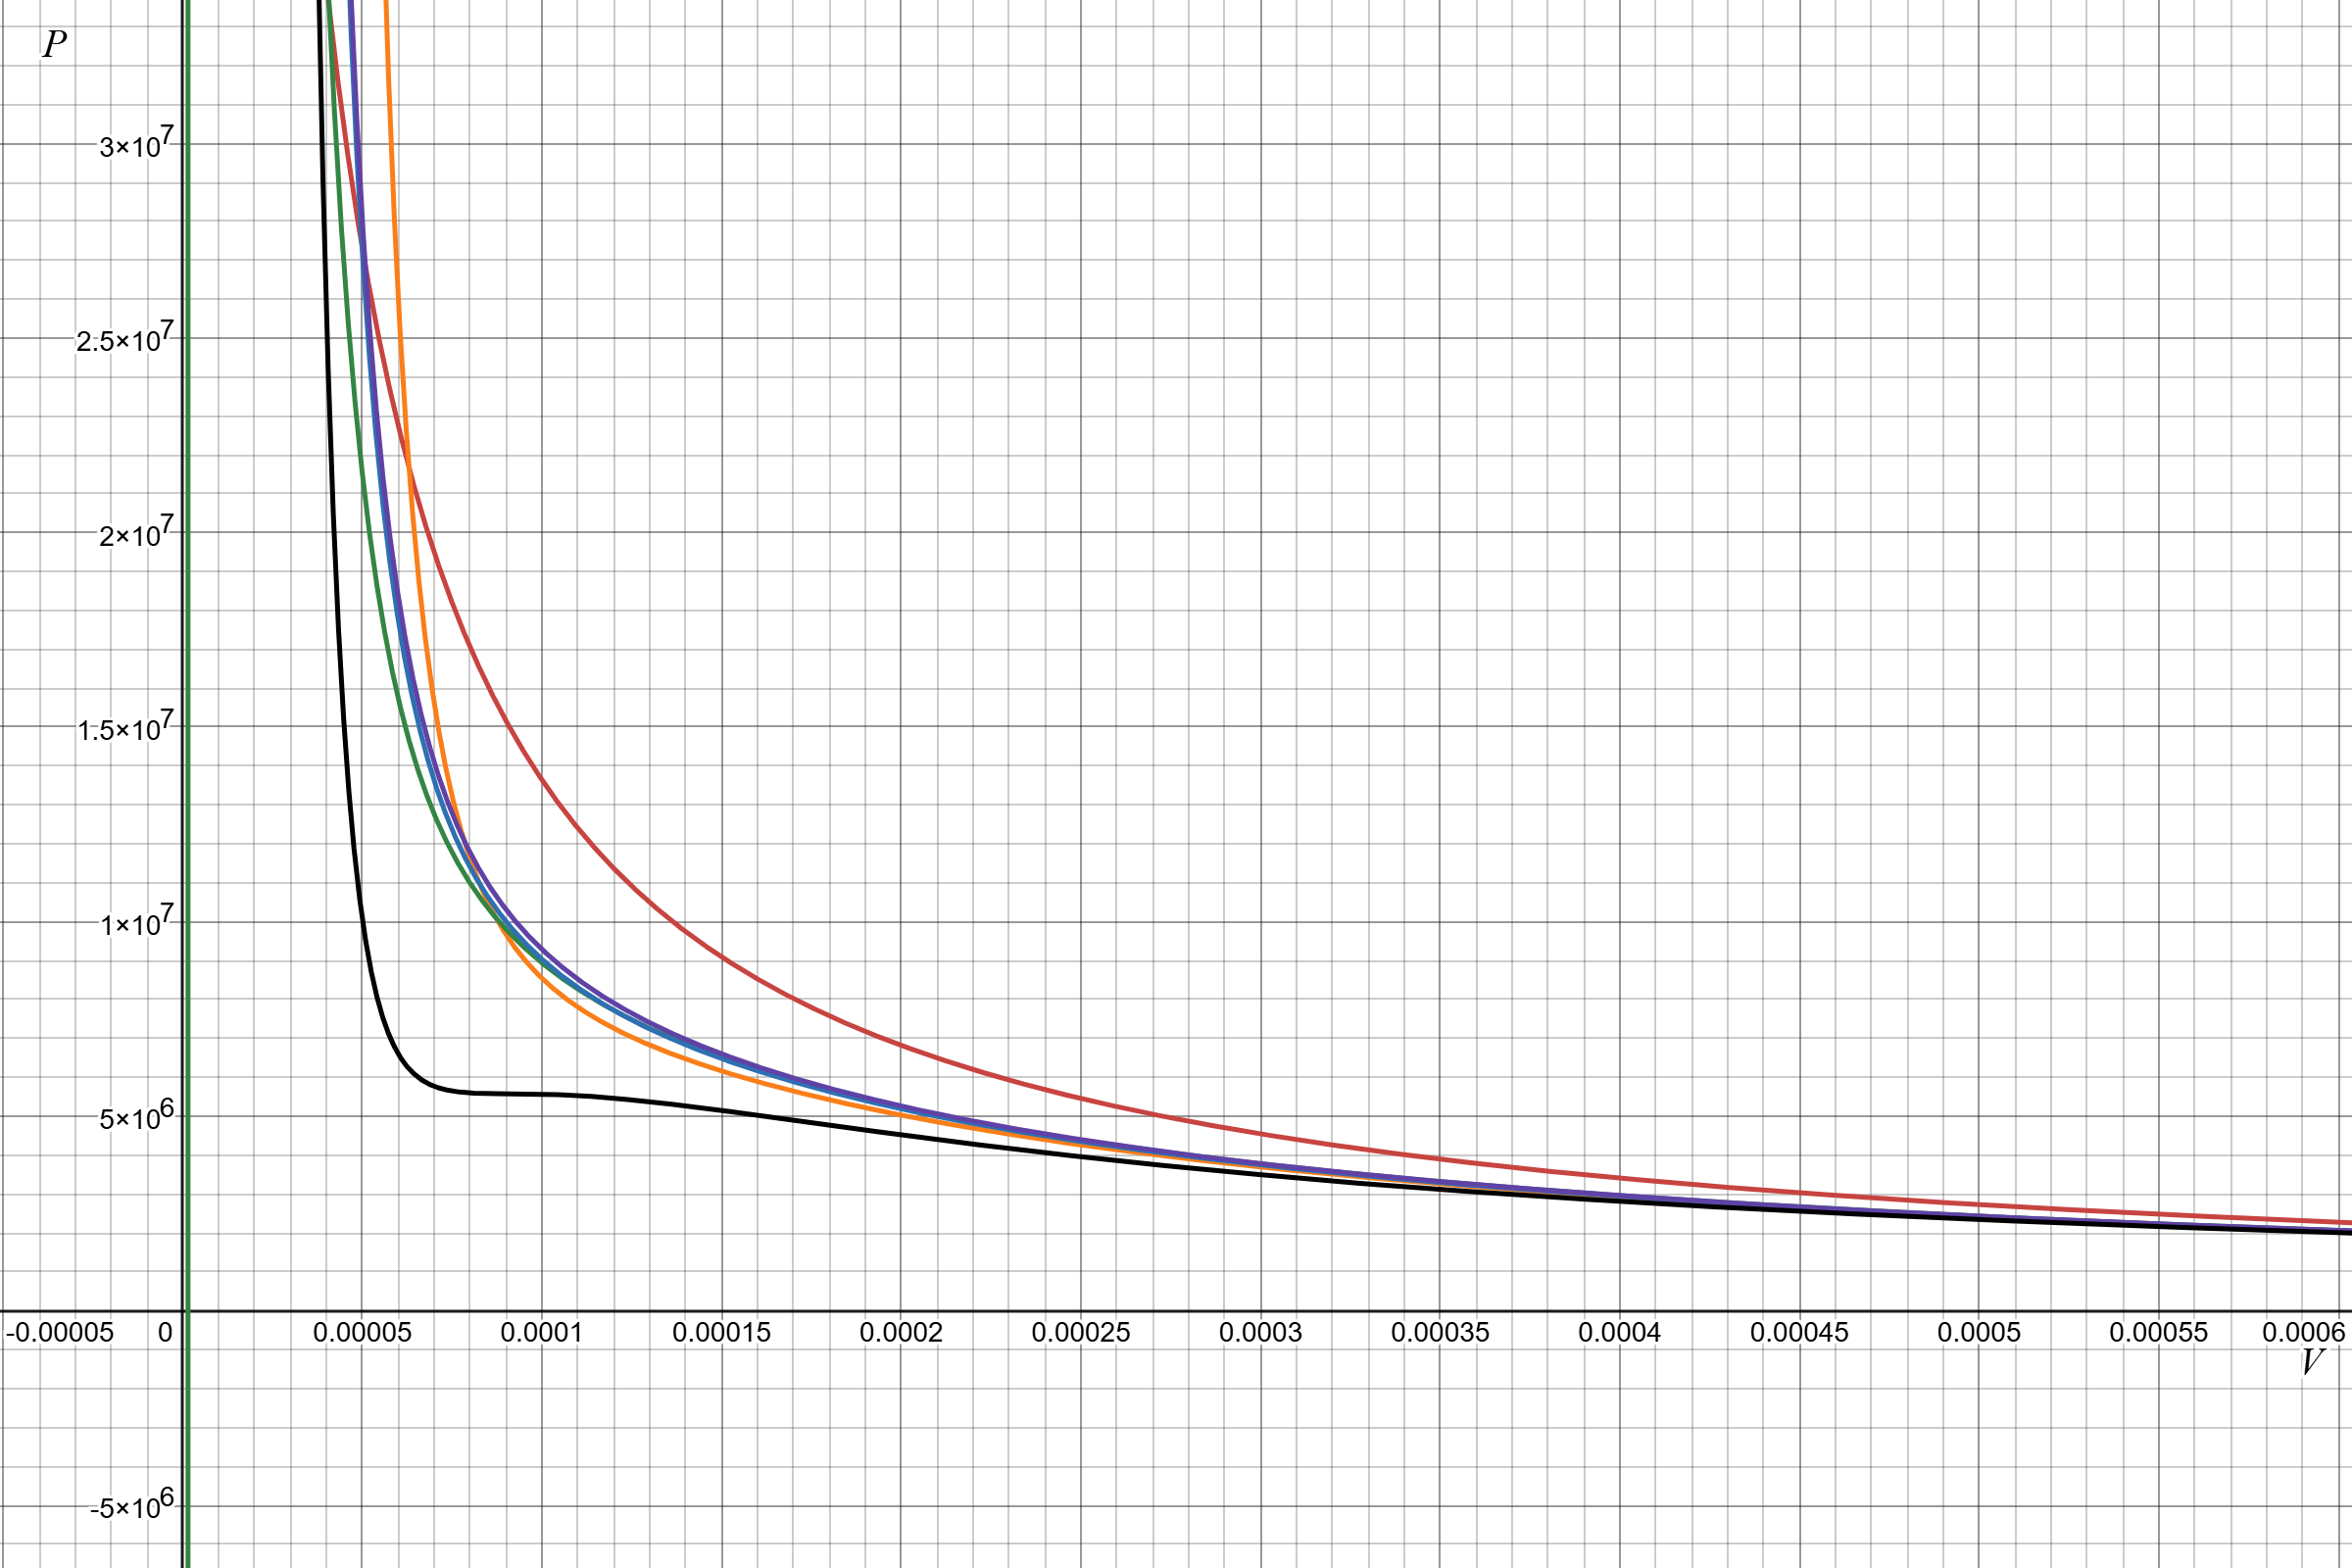
\includegraphics[width=\linewidth]{Graphics/N2/164.png}
        \caption{\label{fig:clausius_1}График 7. $P-V$ сравнительное построение графиков уравнений состояния азота $N_2$, $T = 164 \ \text{K}$}
    \end{minipage}
\end{figure}

\begin{figure}[h!]
    \centering
    \begin{minipage}{0.49\textwidth}
        \centering
        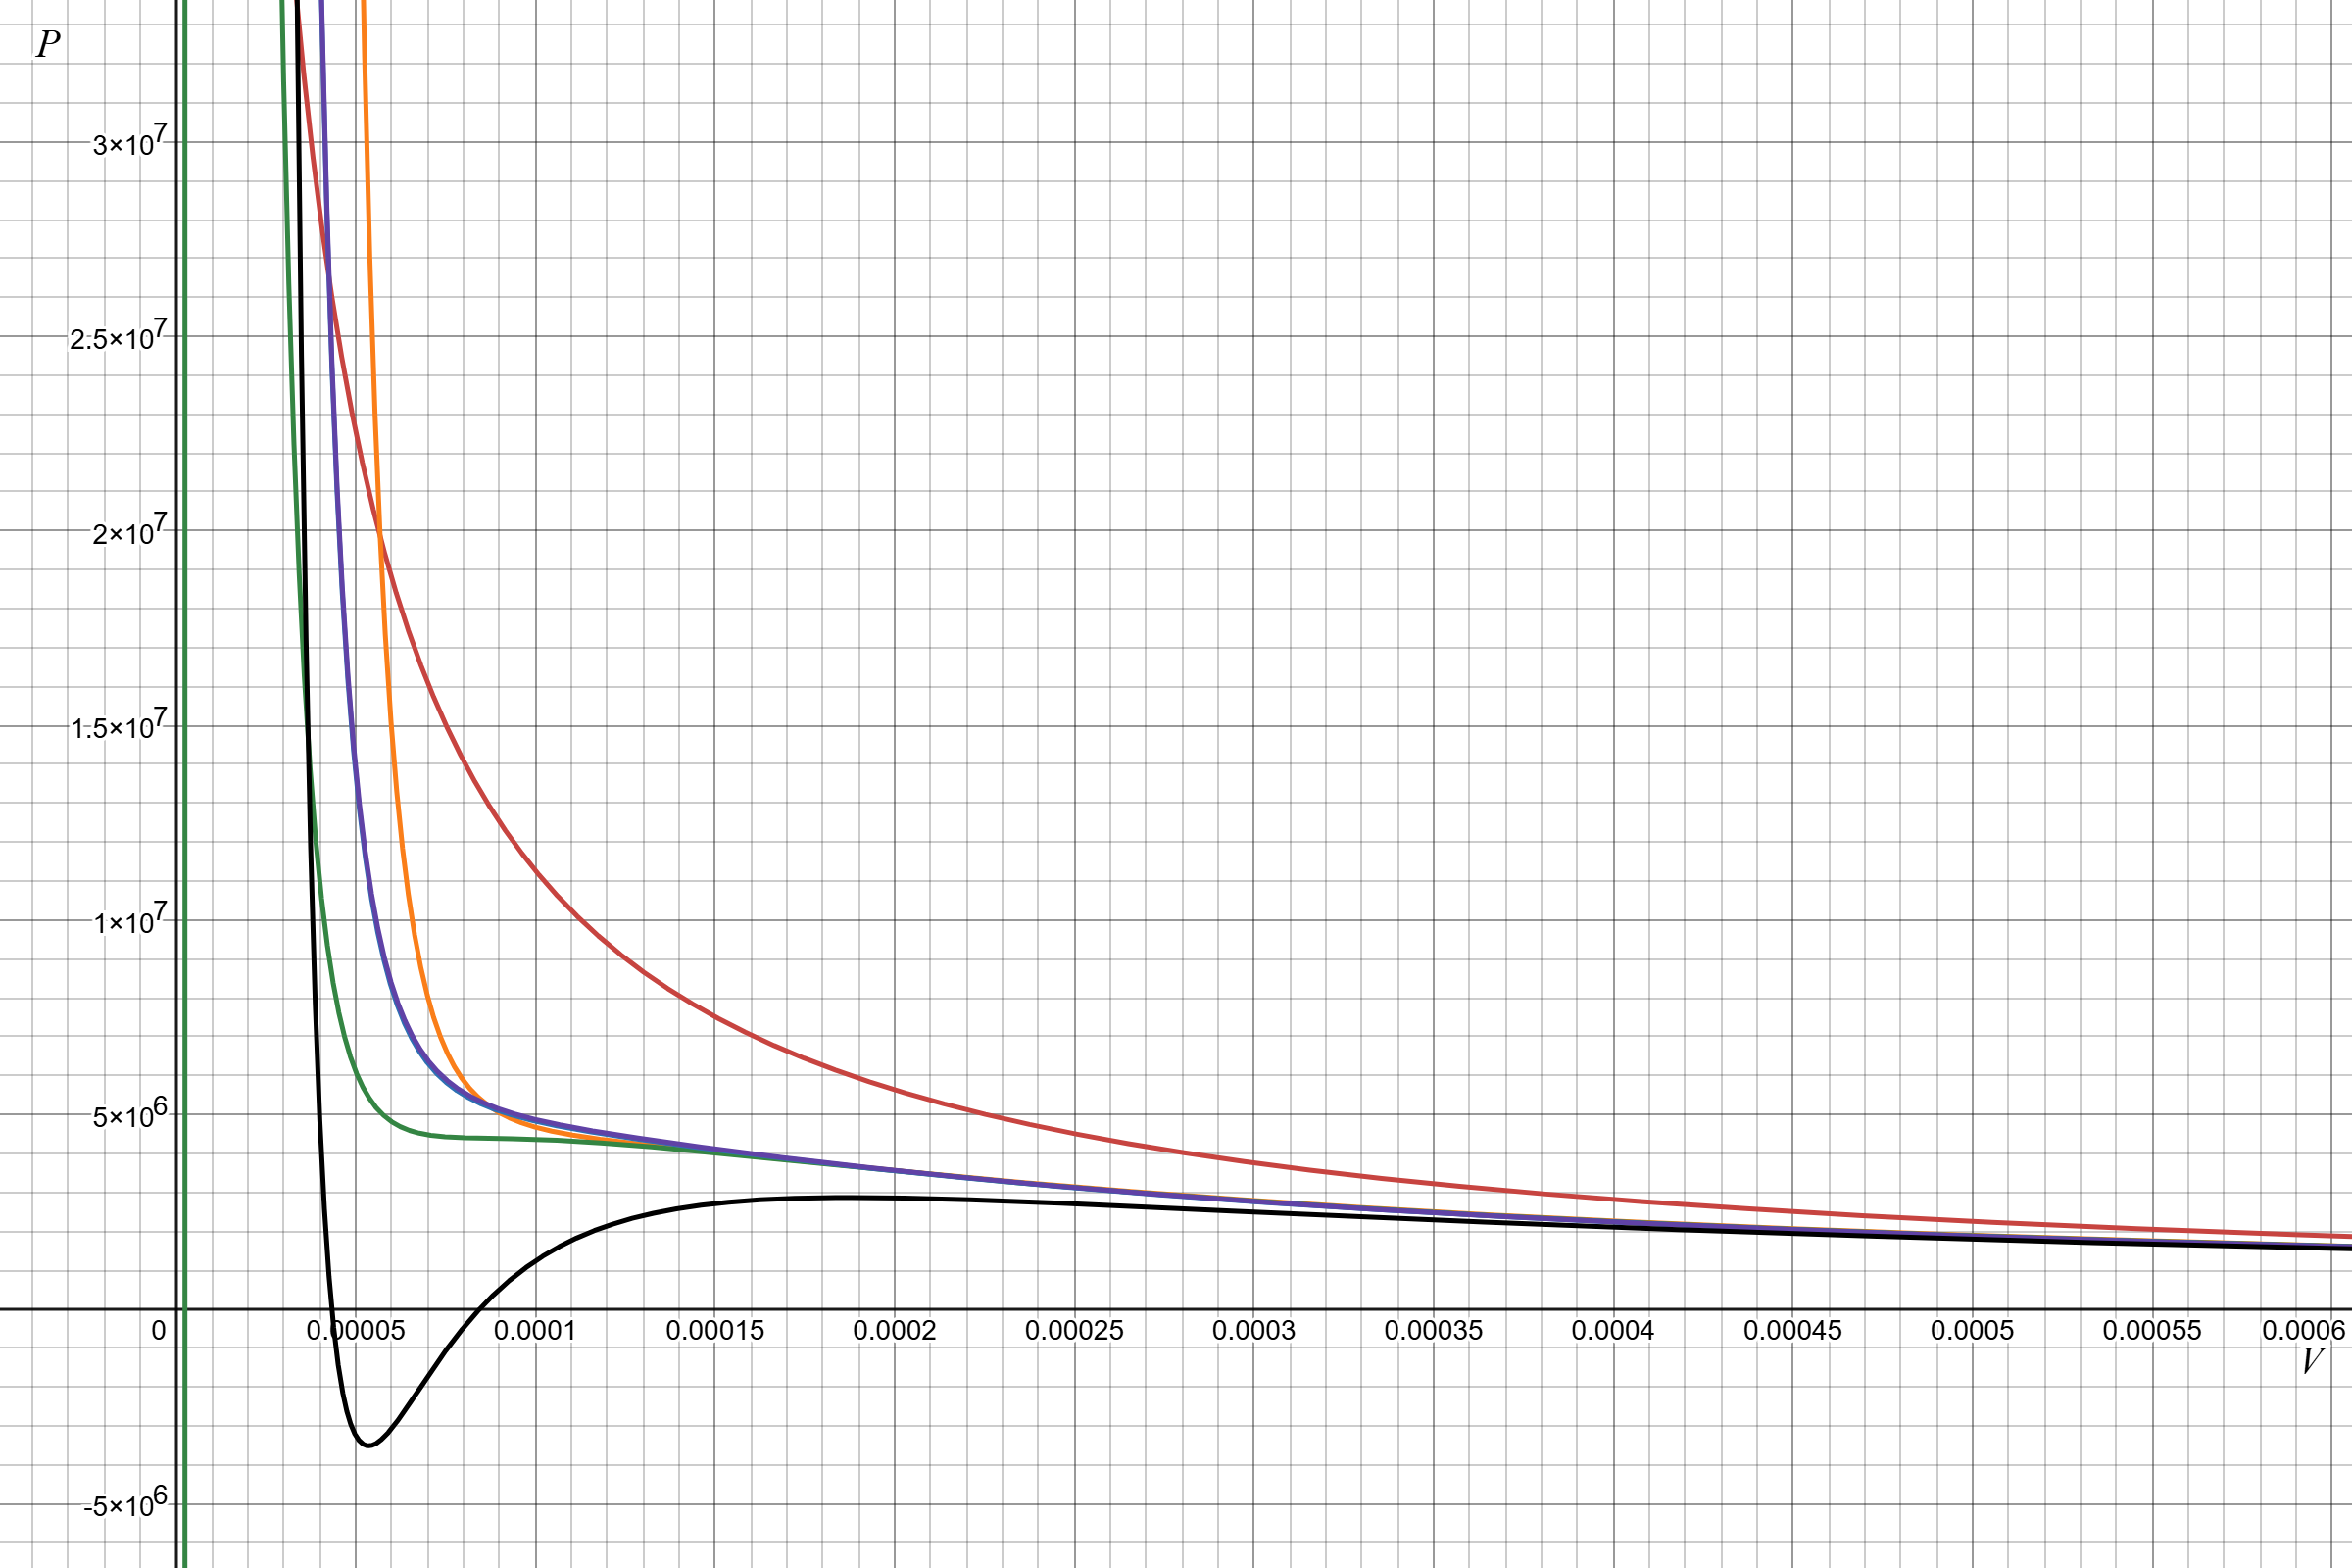
\includegraphics[width=\linewidth]{Graphics/N2/135_5.png}
        \caption{\label{fig:clausius_1}График 8. $P-V$ сравнительное построение графиков уравнений состояния азота $N_2$, $T = 135.5 \ \text{K}$}
    \end{minipage}
    \hfill
    \begin{minipage}{0.49\textwidth}
        \centering
        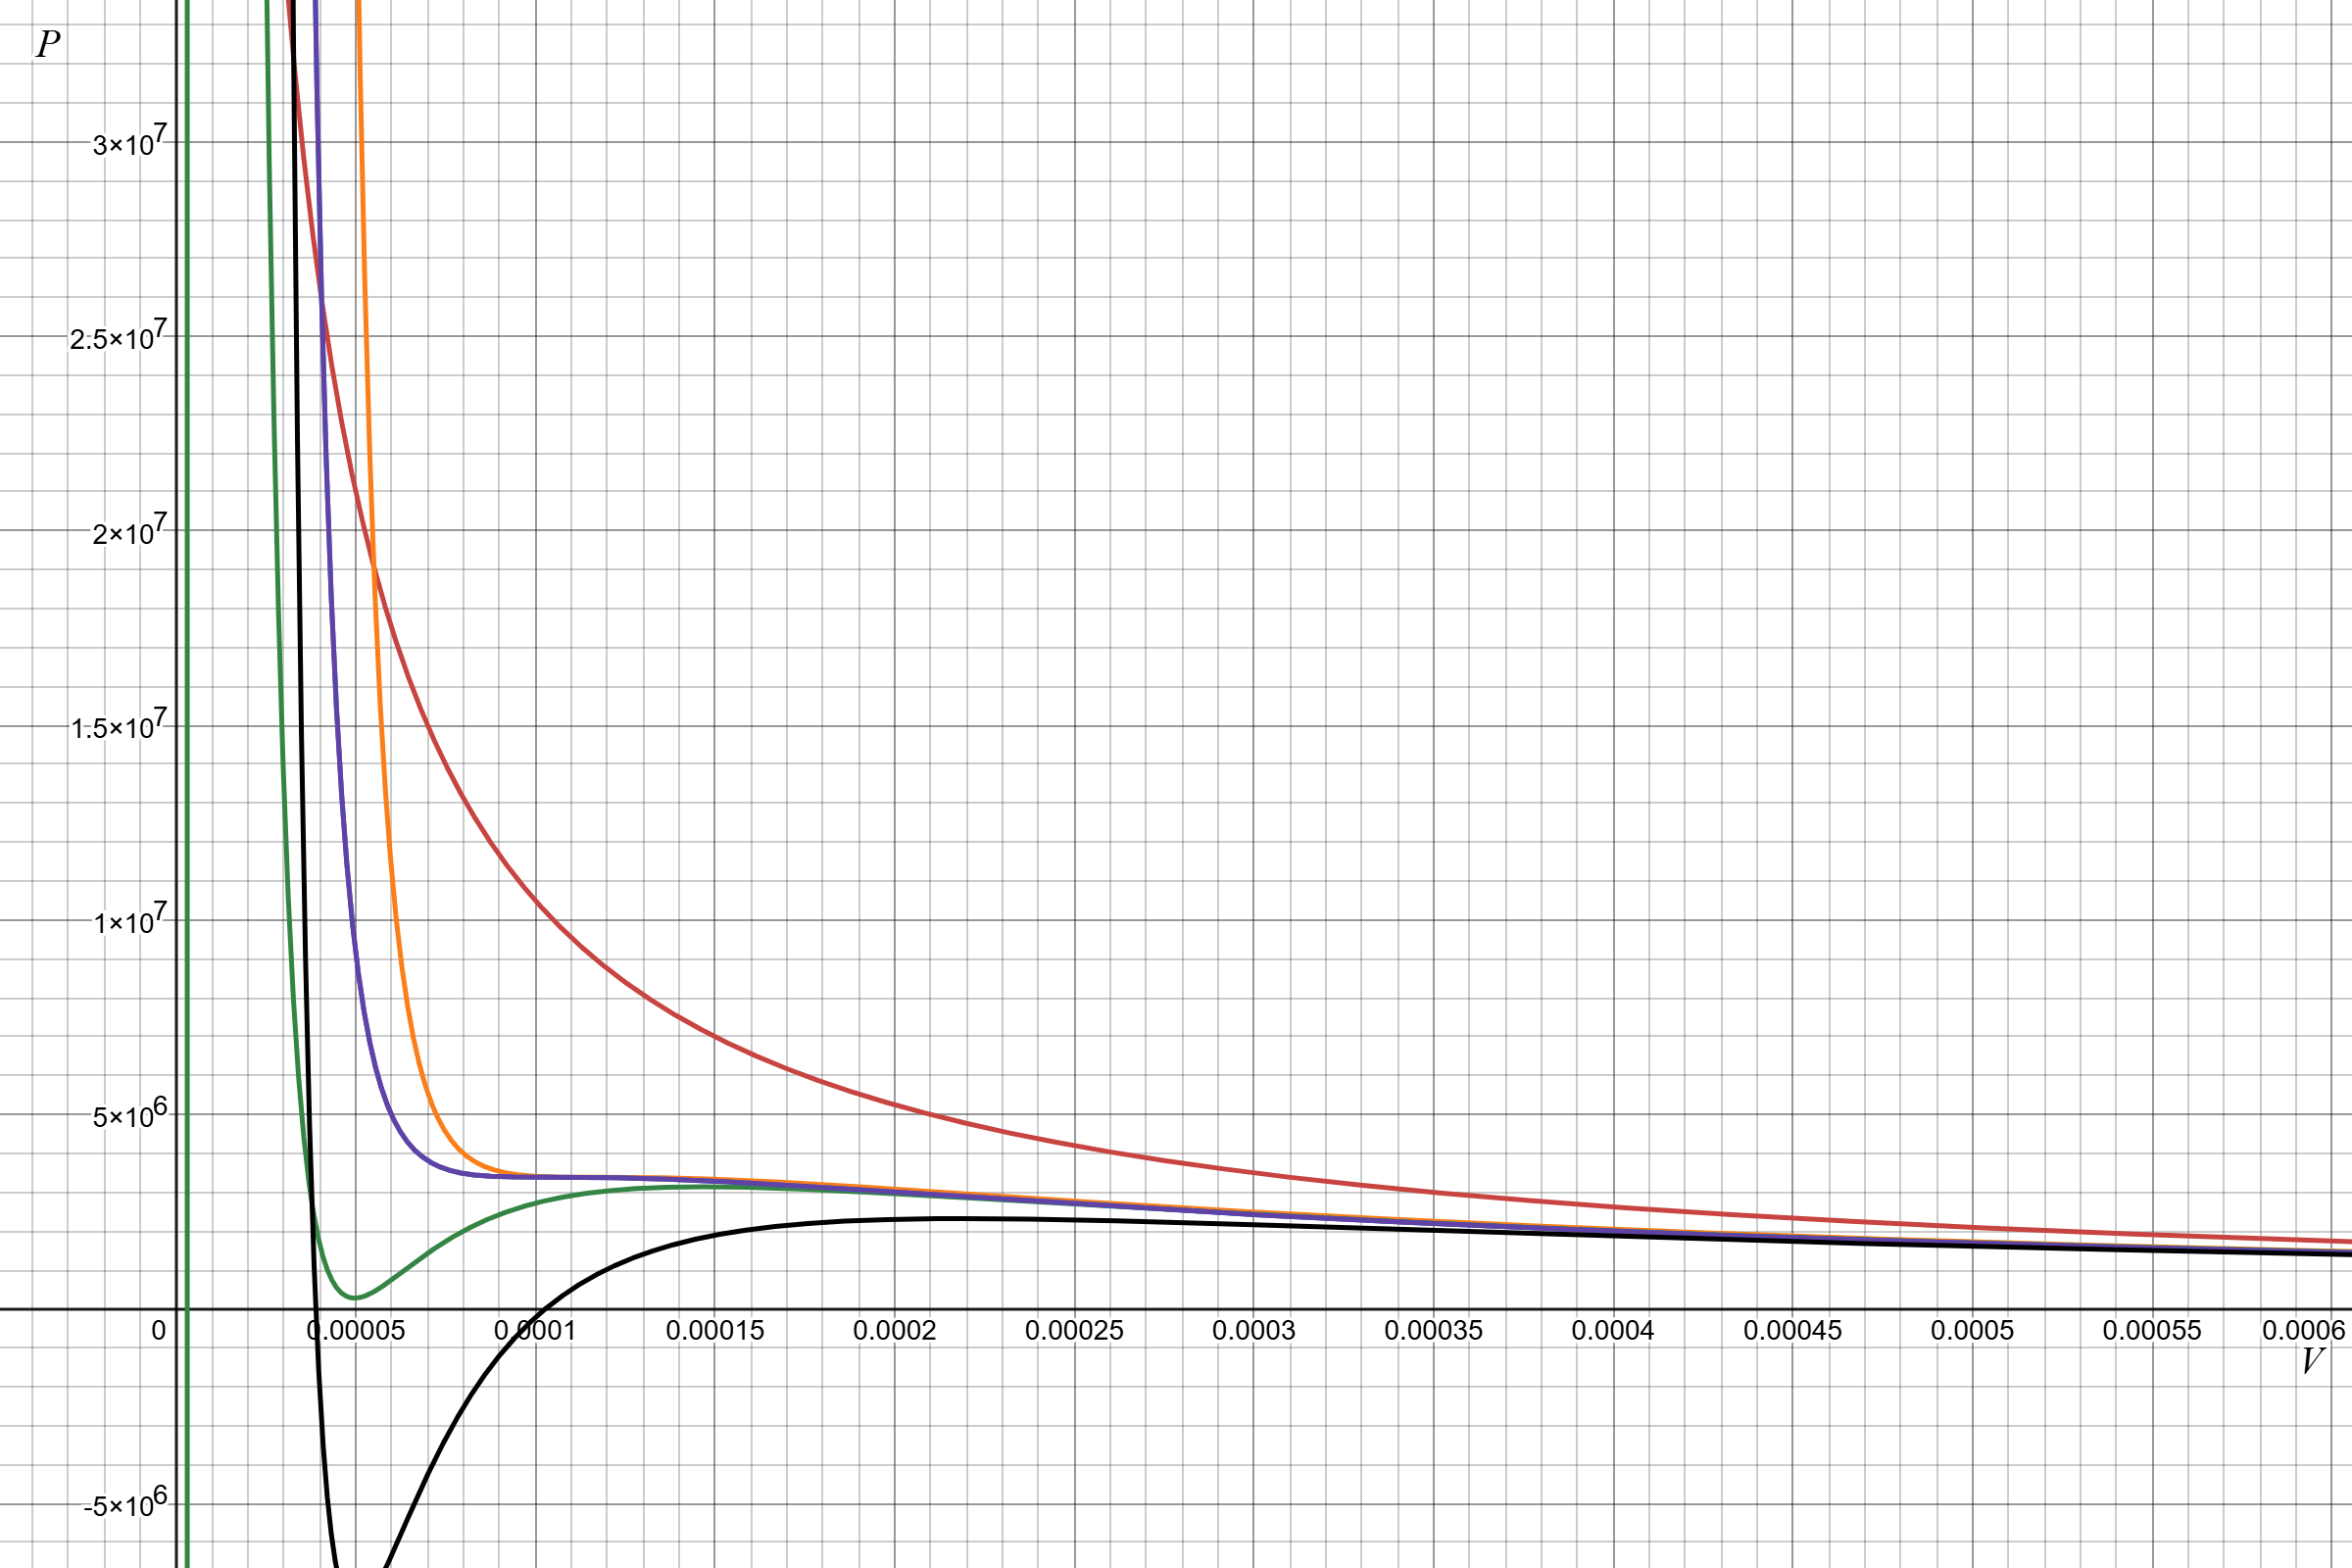
\includegraphics[width=\linewidth]{Graphics/N2/126_21.png}
        \caption{\label{fig:clausius_1}График 9. $P-V$ сравнительное построение графиков уравнений состояния азота $N_2$, $T = 126.21 \ \text{K}$}
    \end{minipage}
\end{figure}
\begin{figure}[h!]
    \centering
    \begin{minipage}{0.49\textwidth}
        \centering
        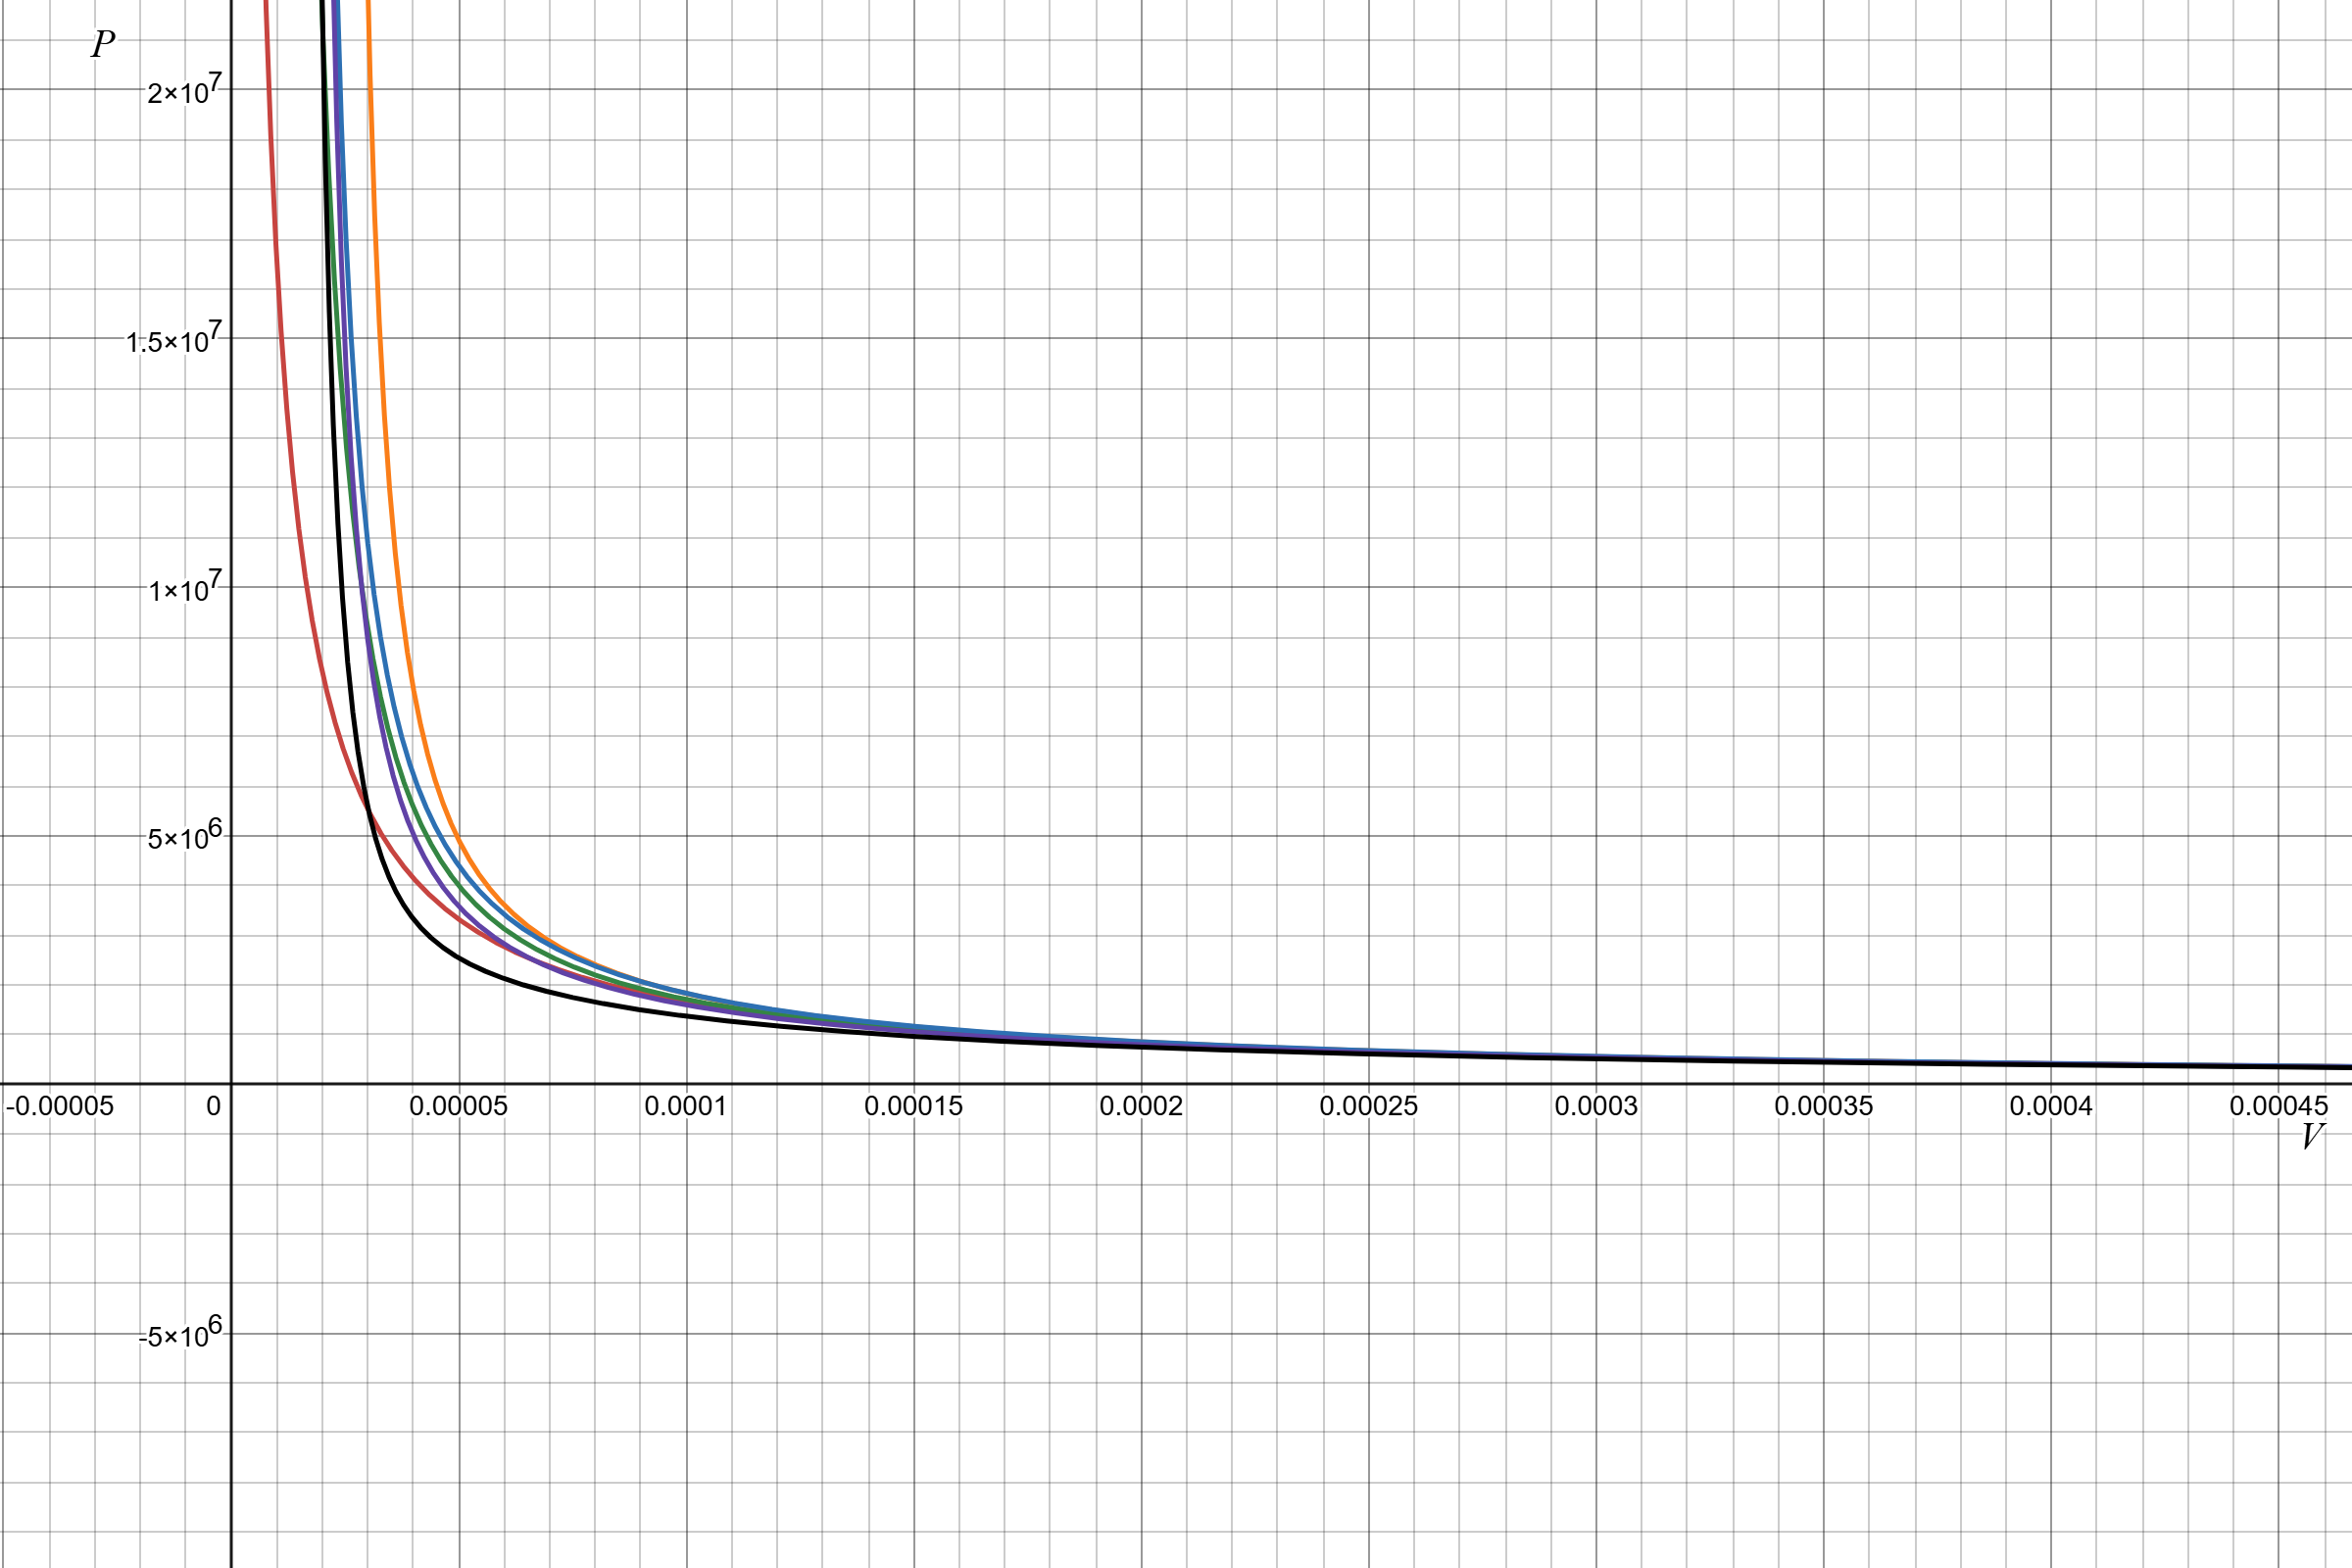
\includegraphics[width=\linewidth]{Graphics/He/20.png}
        \caption{\label{fig:clausius_1}График 10. $P-V$ сравнительное построение графиков уравнений состояния гелия $He$, $T = 20 \ \text{K}$}
    \end{minipage}
    \hfill
    \begin{minipage}{0.49\textwidth}
        \centering
        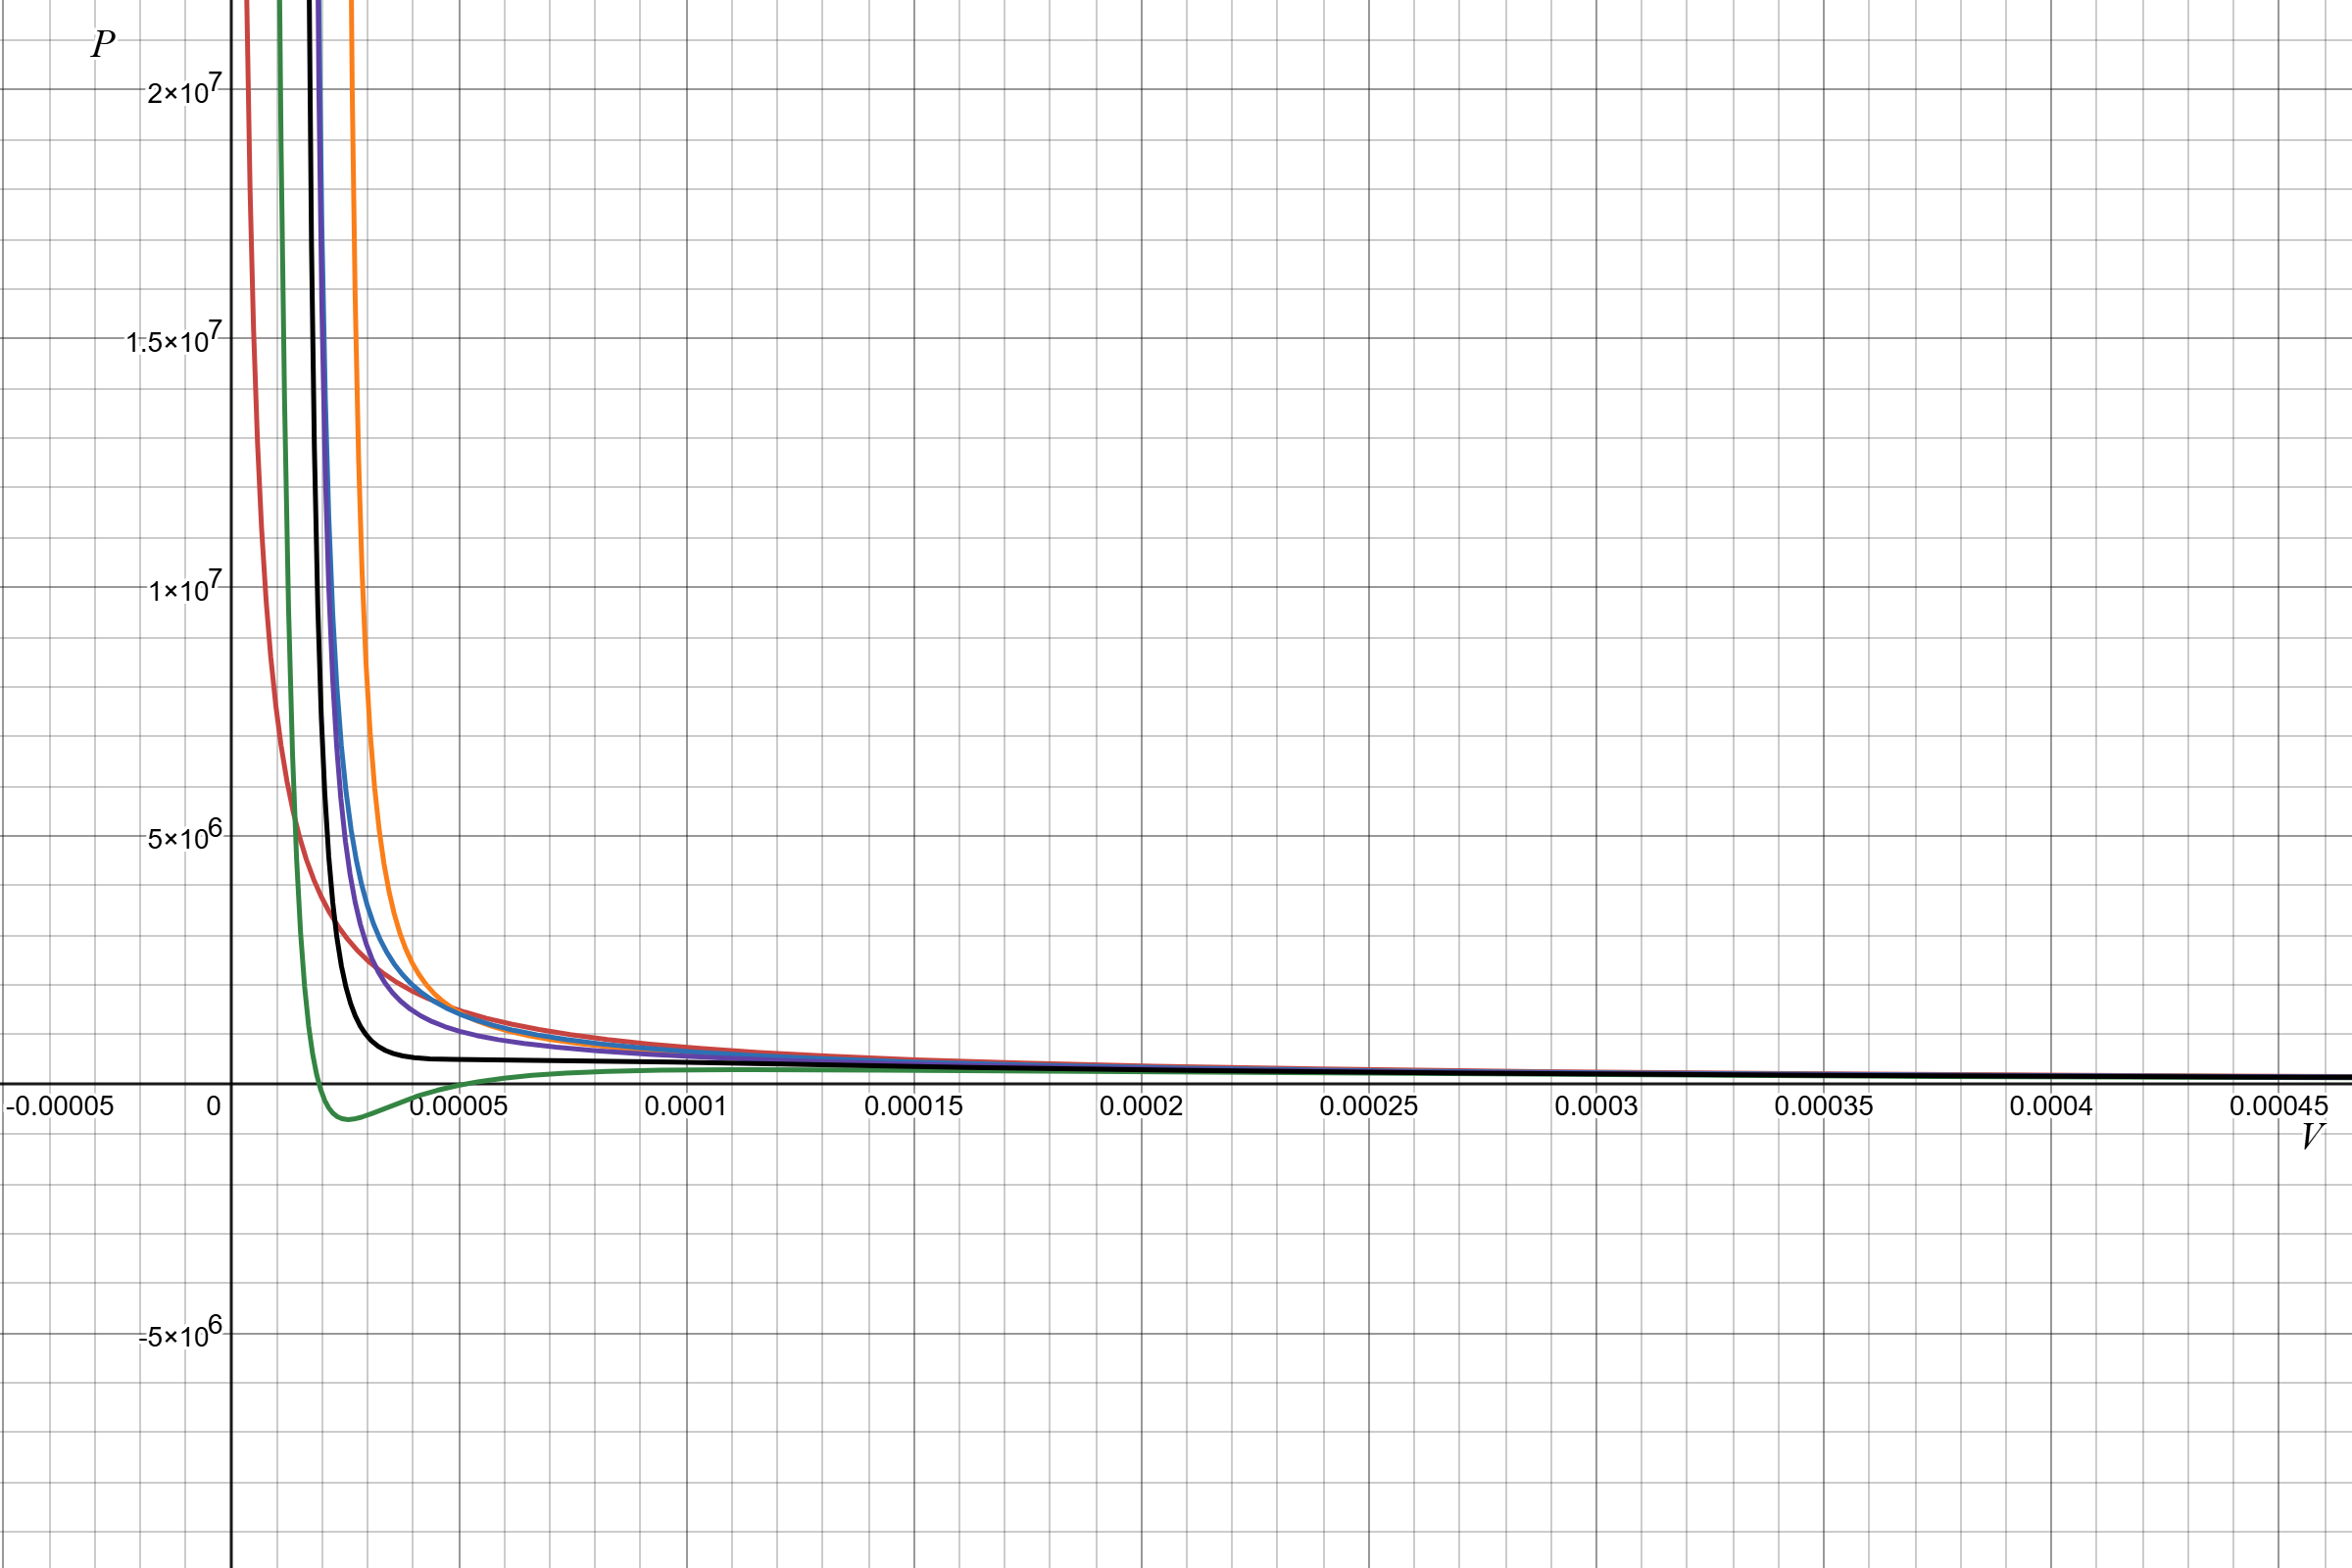
\includegraphics[width=\linewidth]{Graphics/He/9.png}
        \caption{\label{fig:clausius_1}График 11. $P-V$ сравнительное построение графиков уравнений состояния гелия $He$, $T = 9 \ \text{K}$}
    \end{minipage}
\end{figure}
\clearpage
\begin{figure}[h!]
    \centering
    \begin{minipage}{0.49\textwidth}
        \centering
        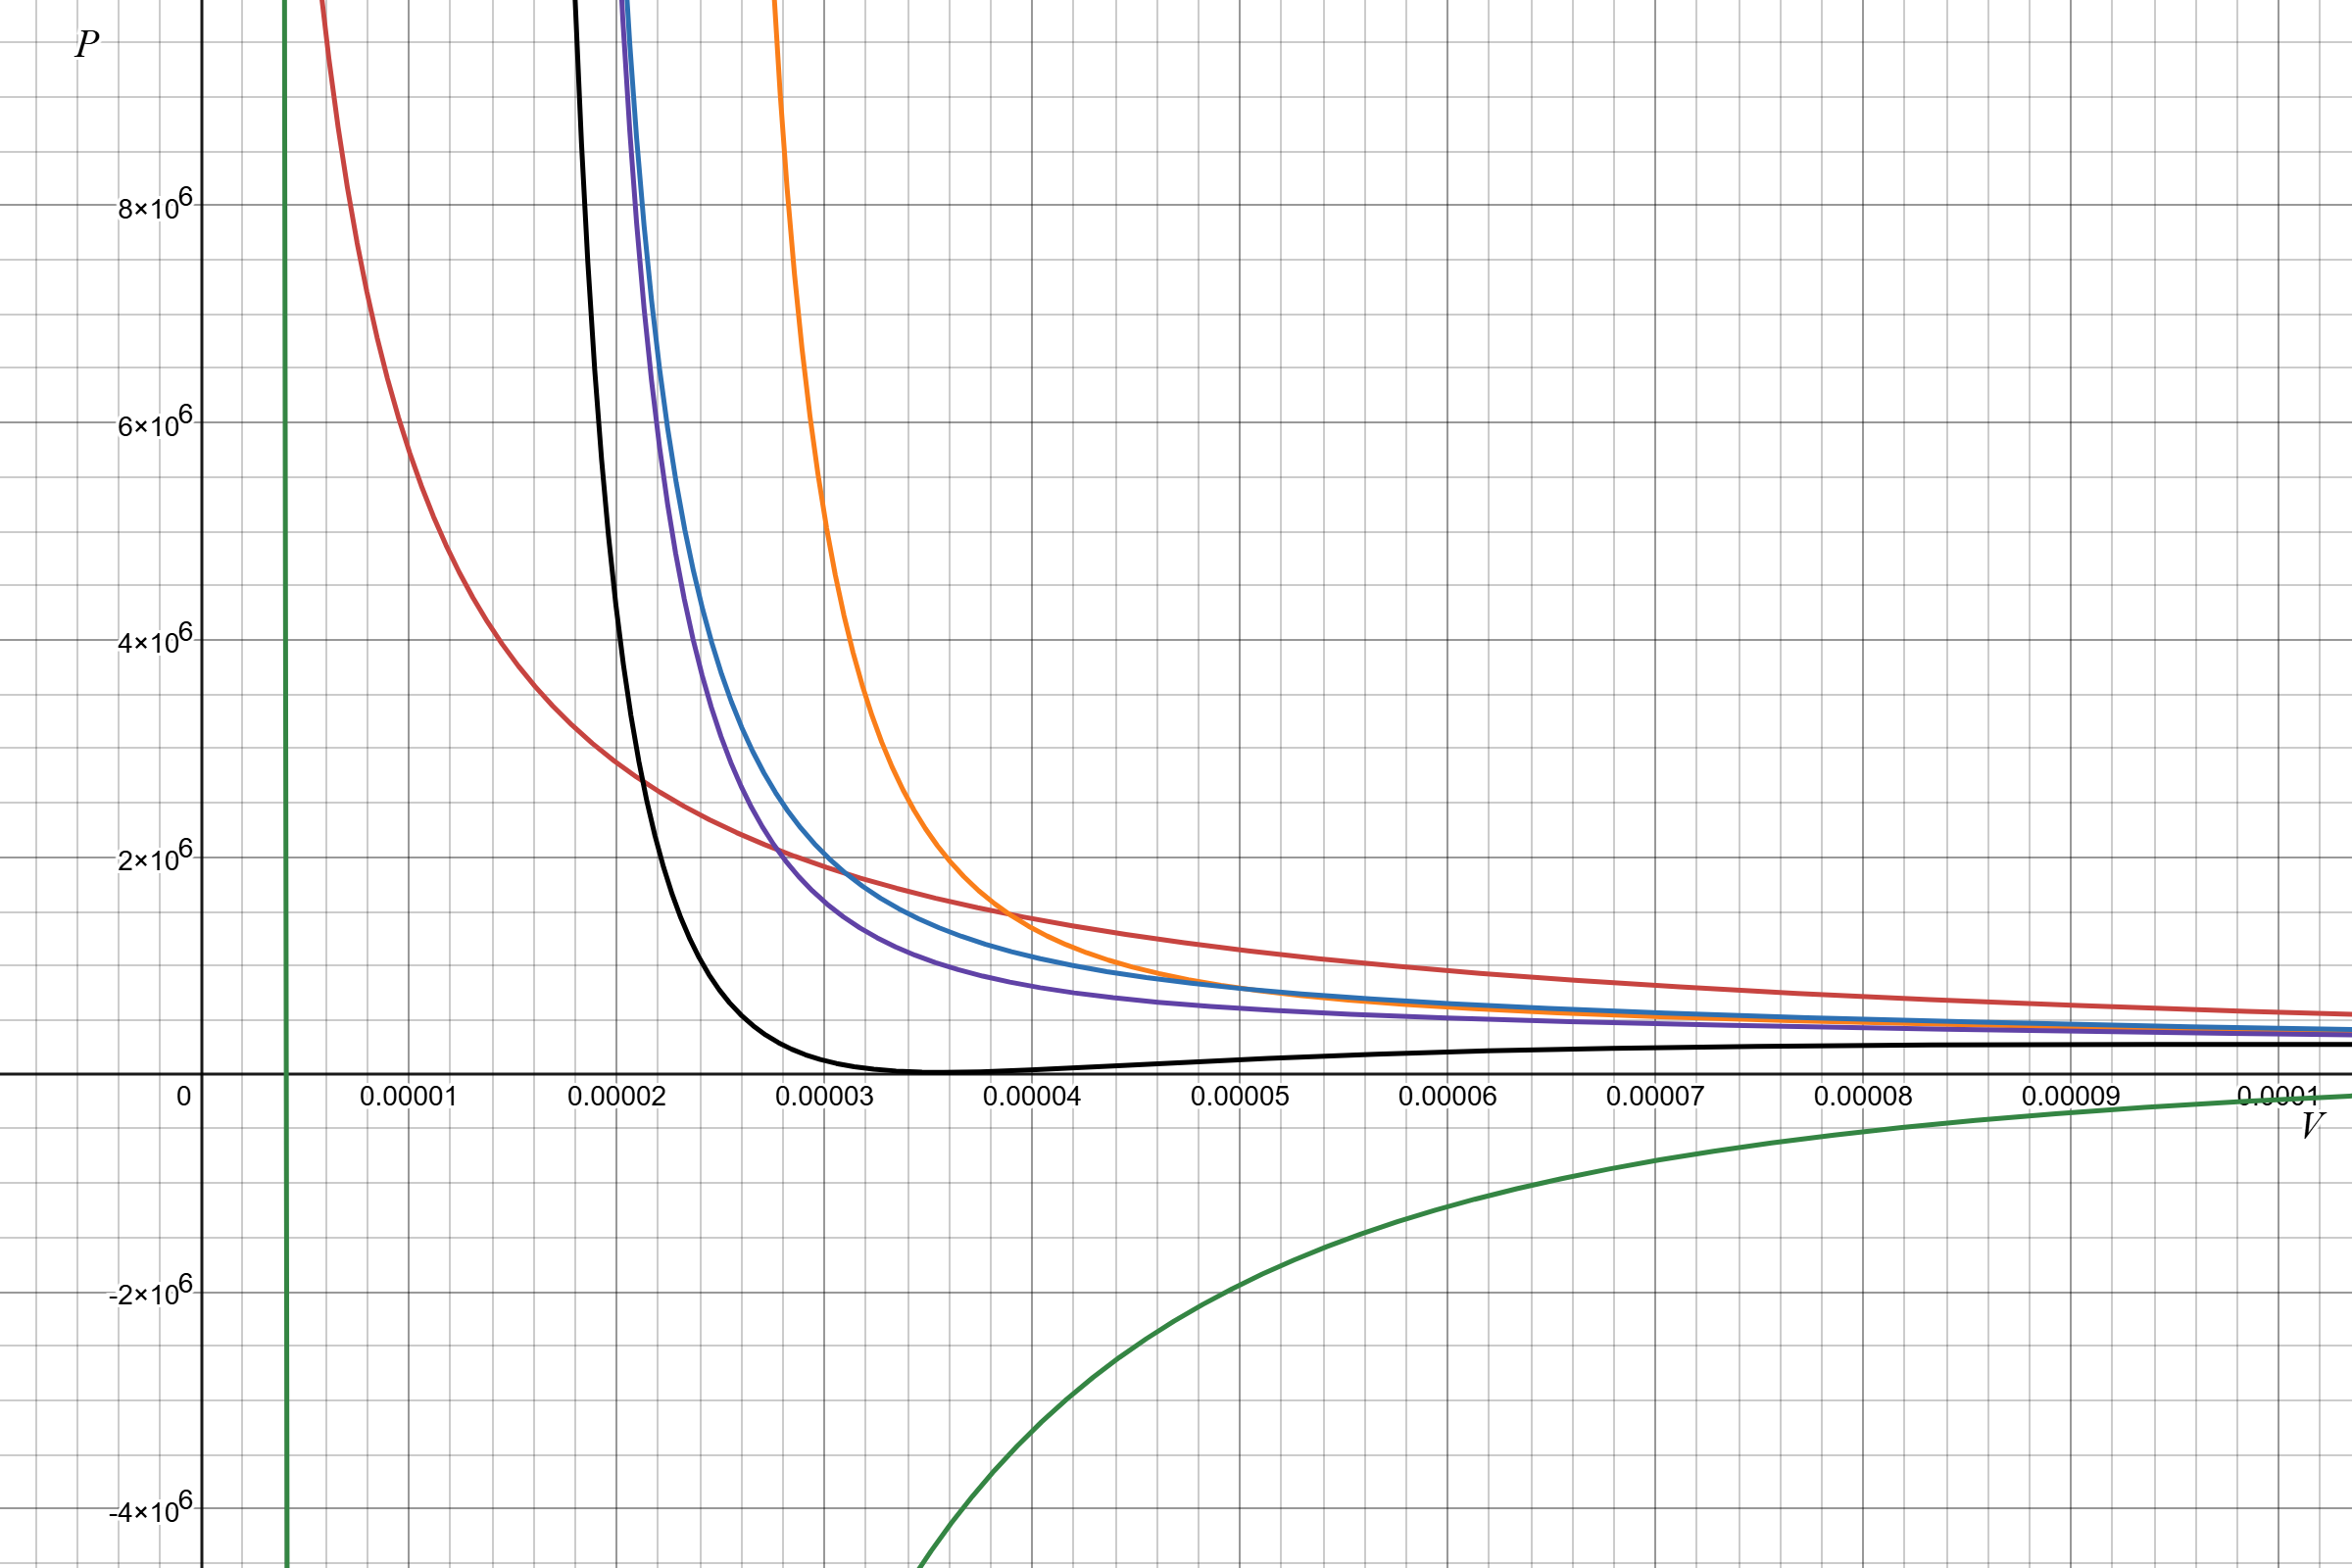
\includegraphics[width=\linewidth]{Graphics/He/6_9.png}
        \caption{\label{fig:clausius_1}График 12. $P-V$ сравнительное построение графиков уравнений состояния гелия $He$, $T = 6.9 \ \text{K}$}
    \end{minipage}
    \hfill
    \begin{minipage}{0.49\textwidth}
        \centering
        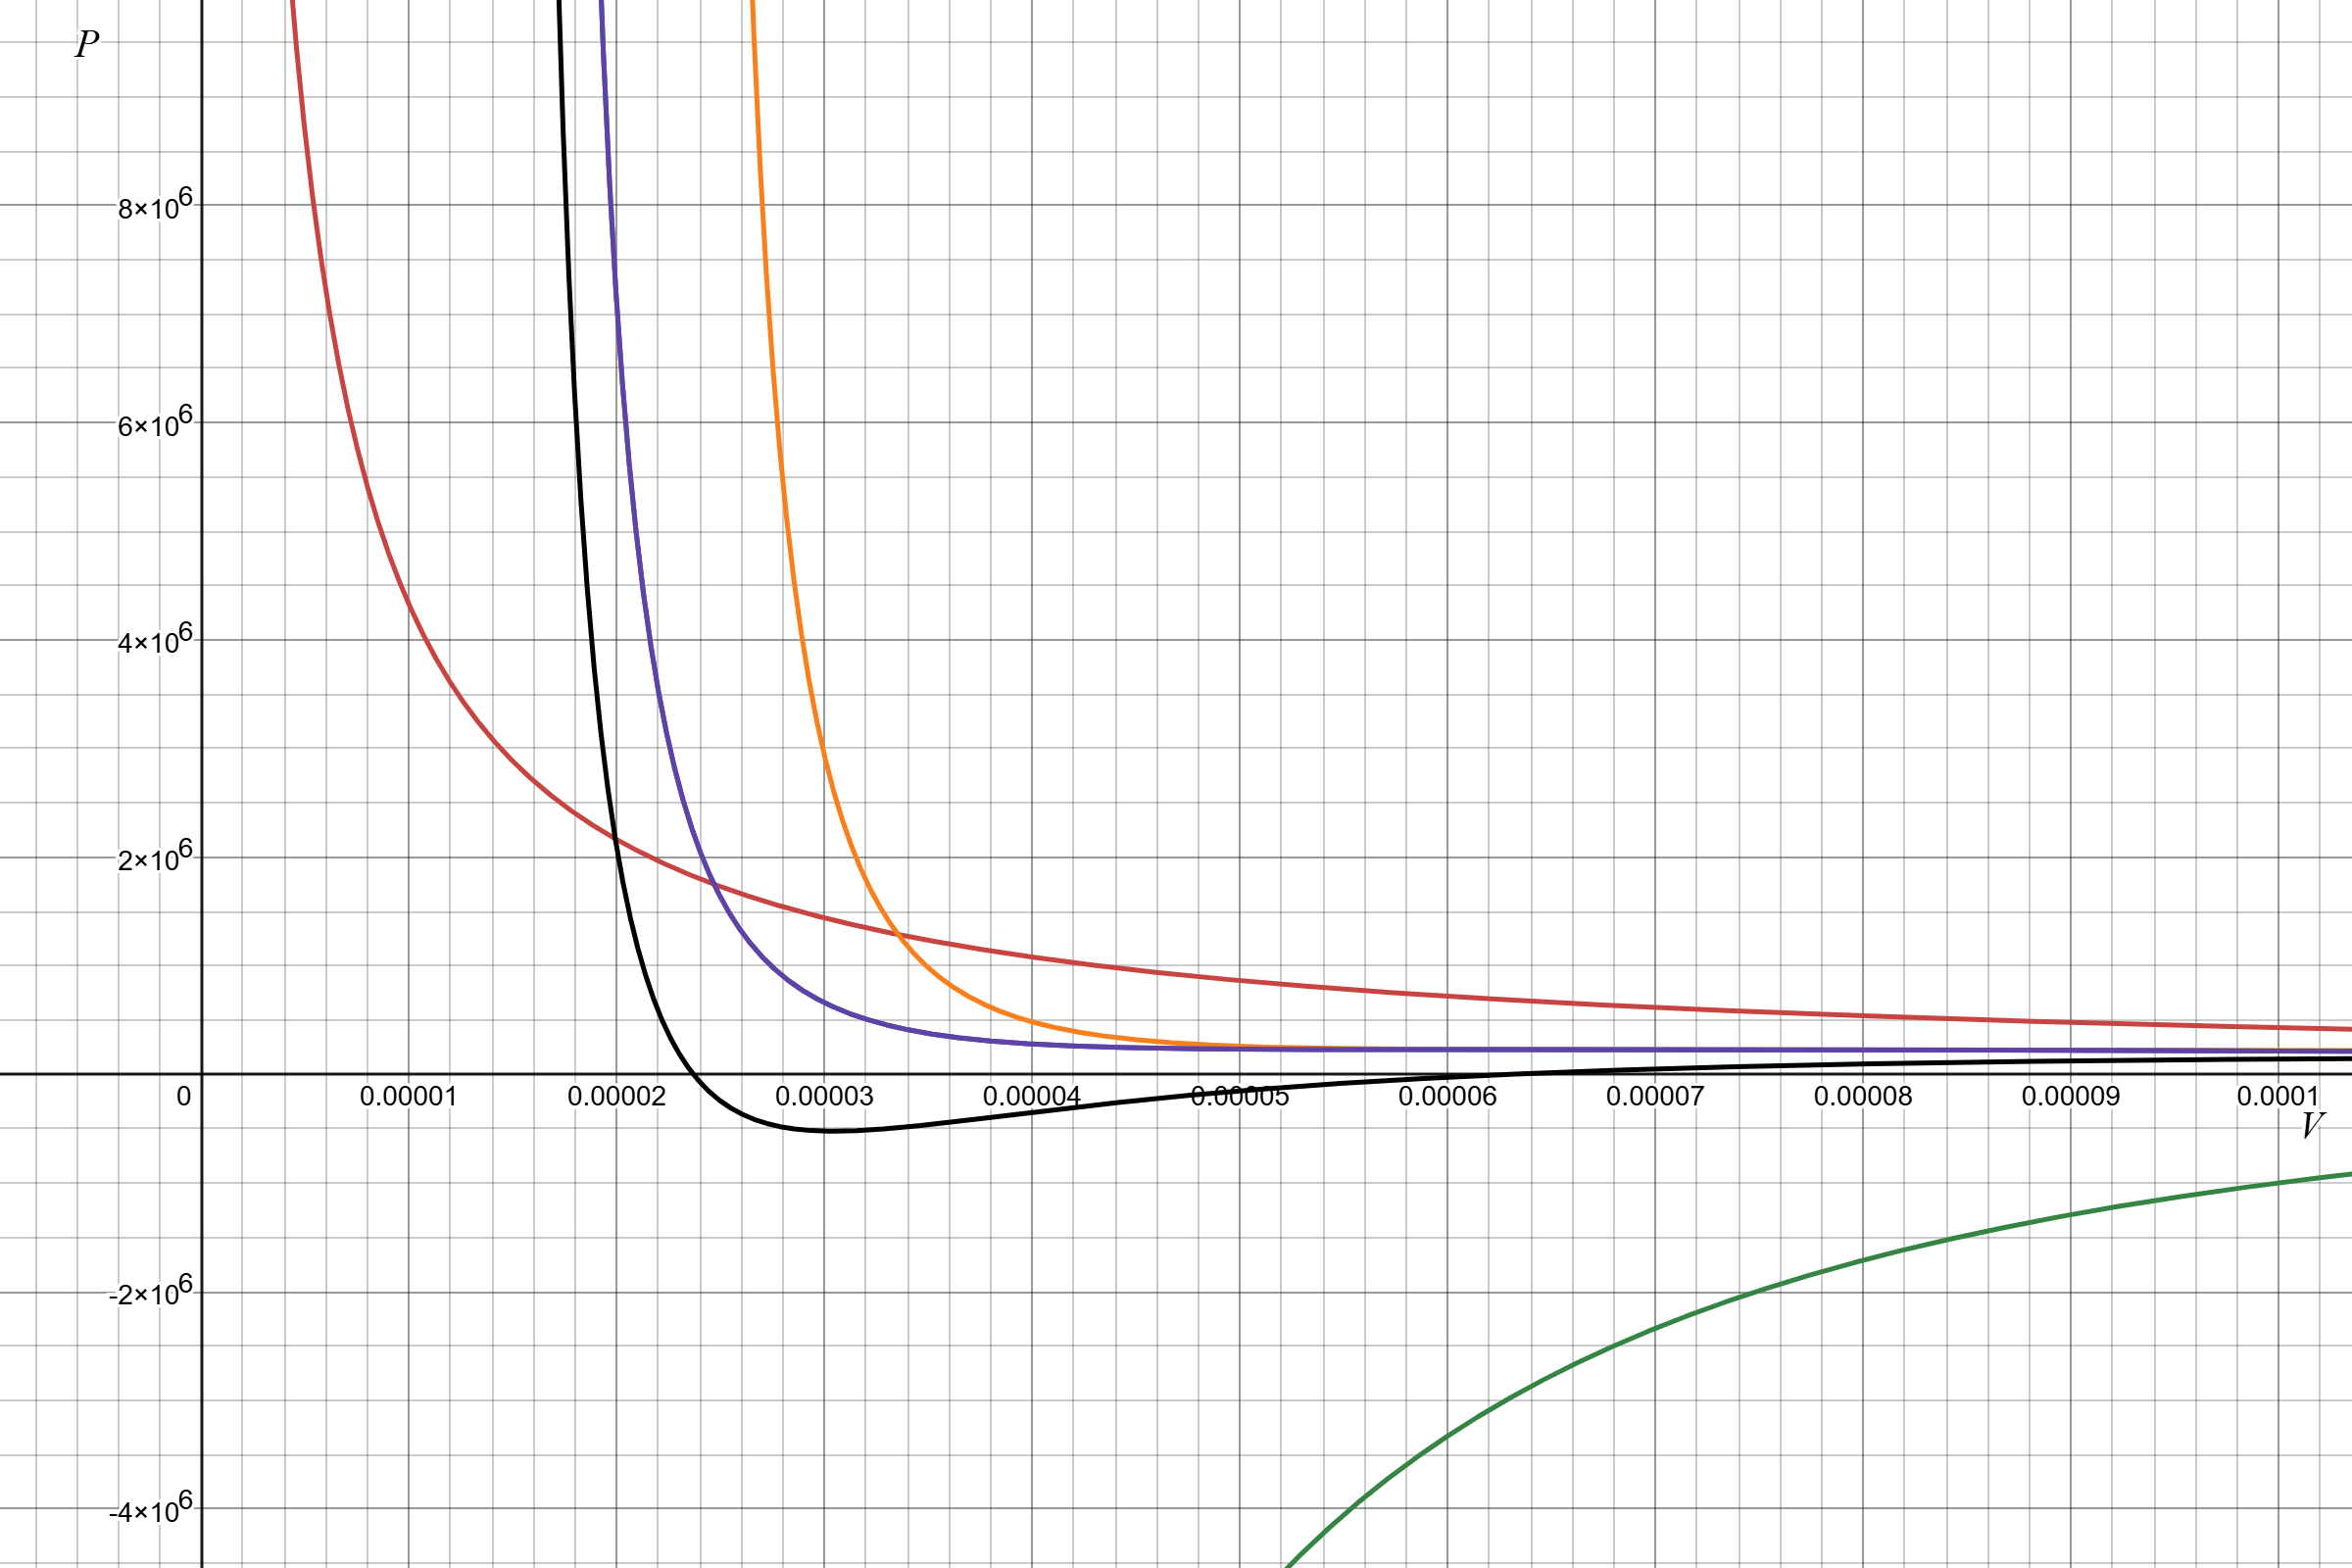
\includegraphics[width=\linewidth]{Graphics/He/5_2.png}
        \caption{\label{fig:clausius_1}График 13. $P-V$ сравнительное построение графиков уравнений состояния гелия $He$, $T = 5.2 \ \text{K}$}
    \end{minipage}
\end{figure}

\begin{figure}[h!]
    \centering
    \begin{minipage}{0.49\textwidth}
        \centering
        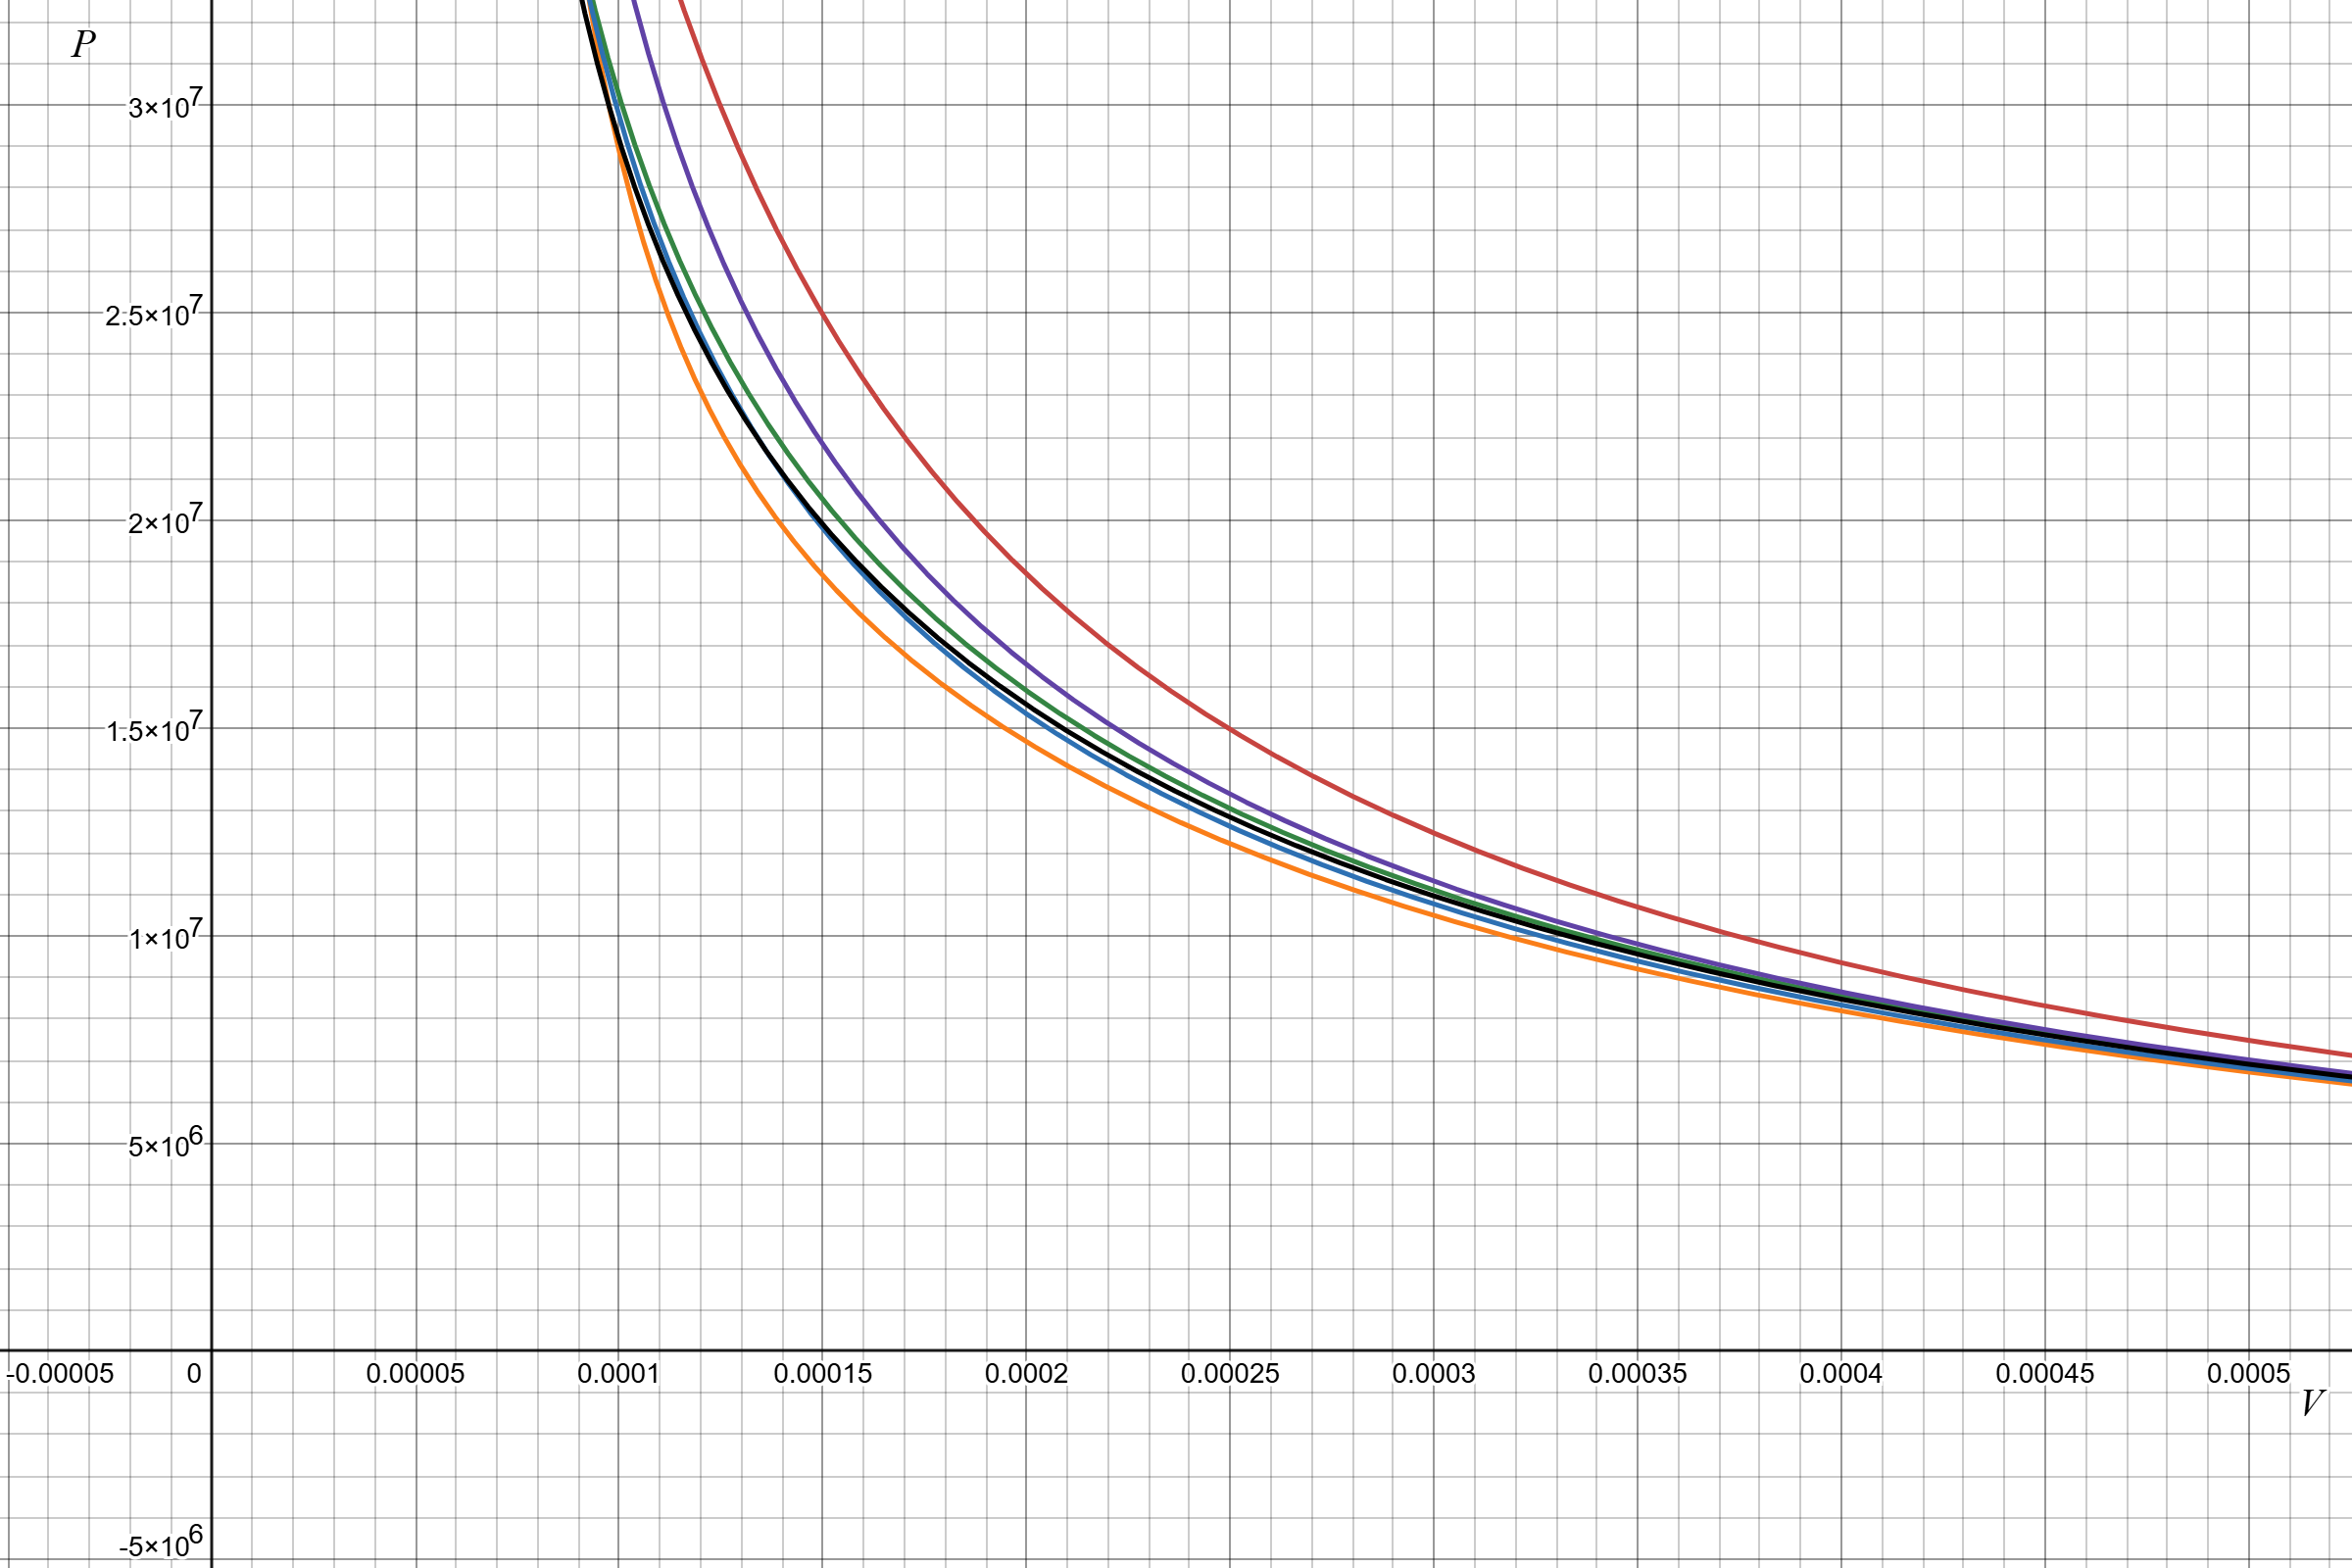
\includegraphics[width=\linewidth]{Graphics/CO2/450.png}
        \caption{\label{fig:clausius_1}График 14. $P-V$ сравнительное построение графиков уравнений состояния углекислого газа $CO_2$, $T = 450 \ \text{K}$}
    \end{minipage}
    \hfill
    \begin{minipage}{0.49\textwidth}
        \centering
        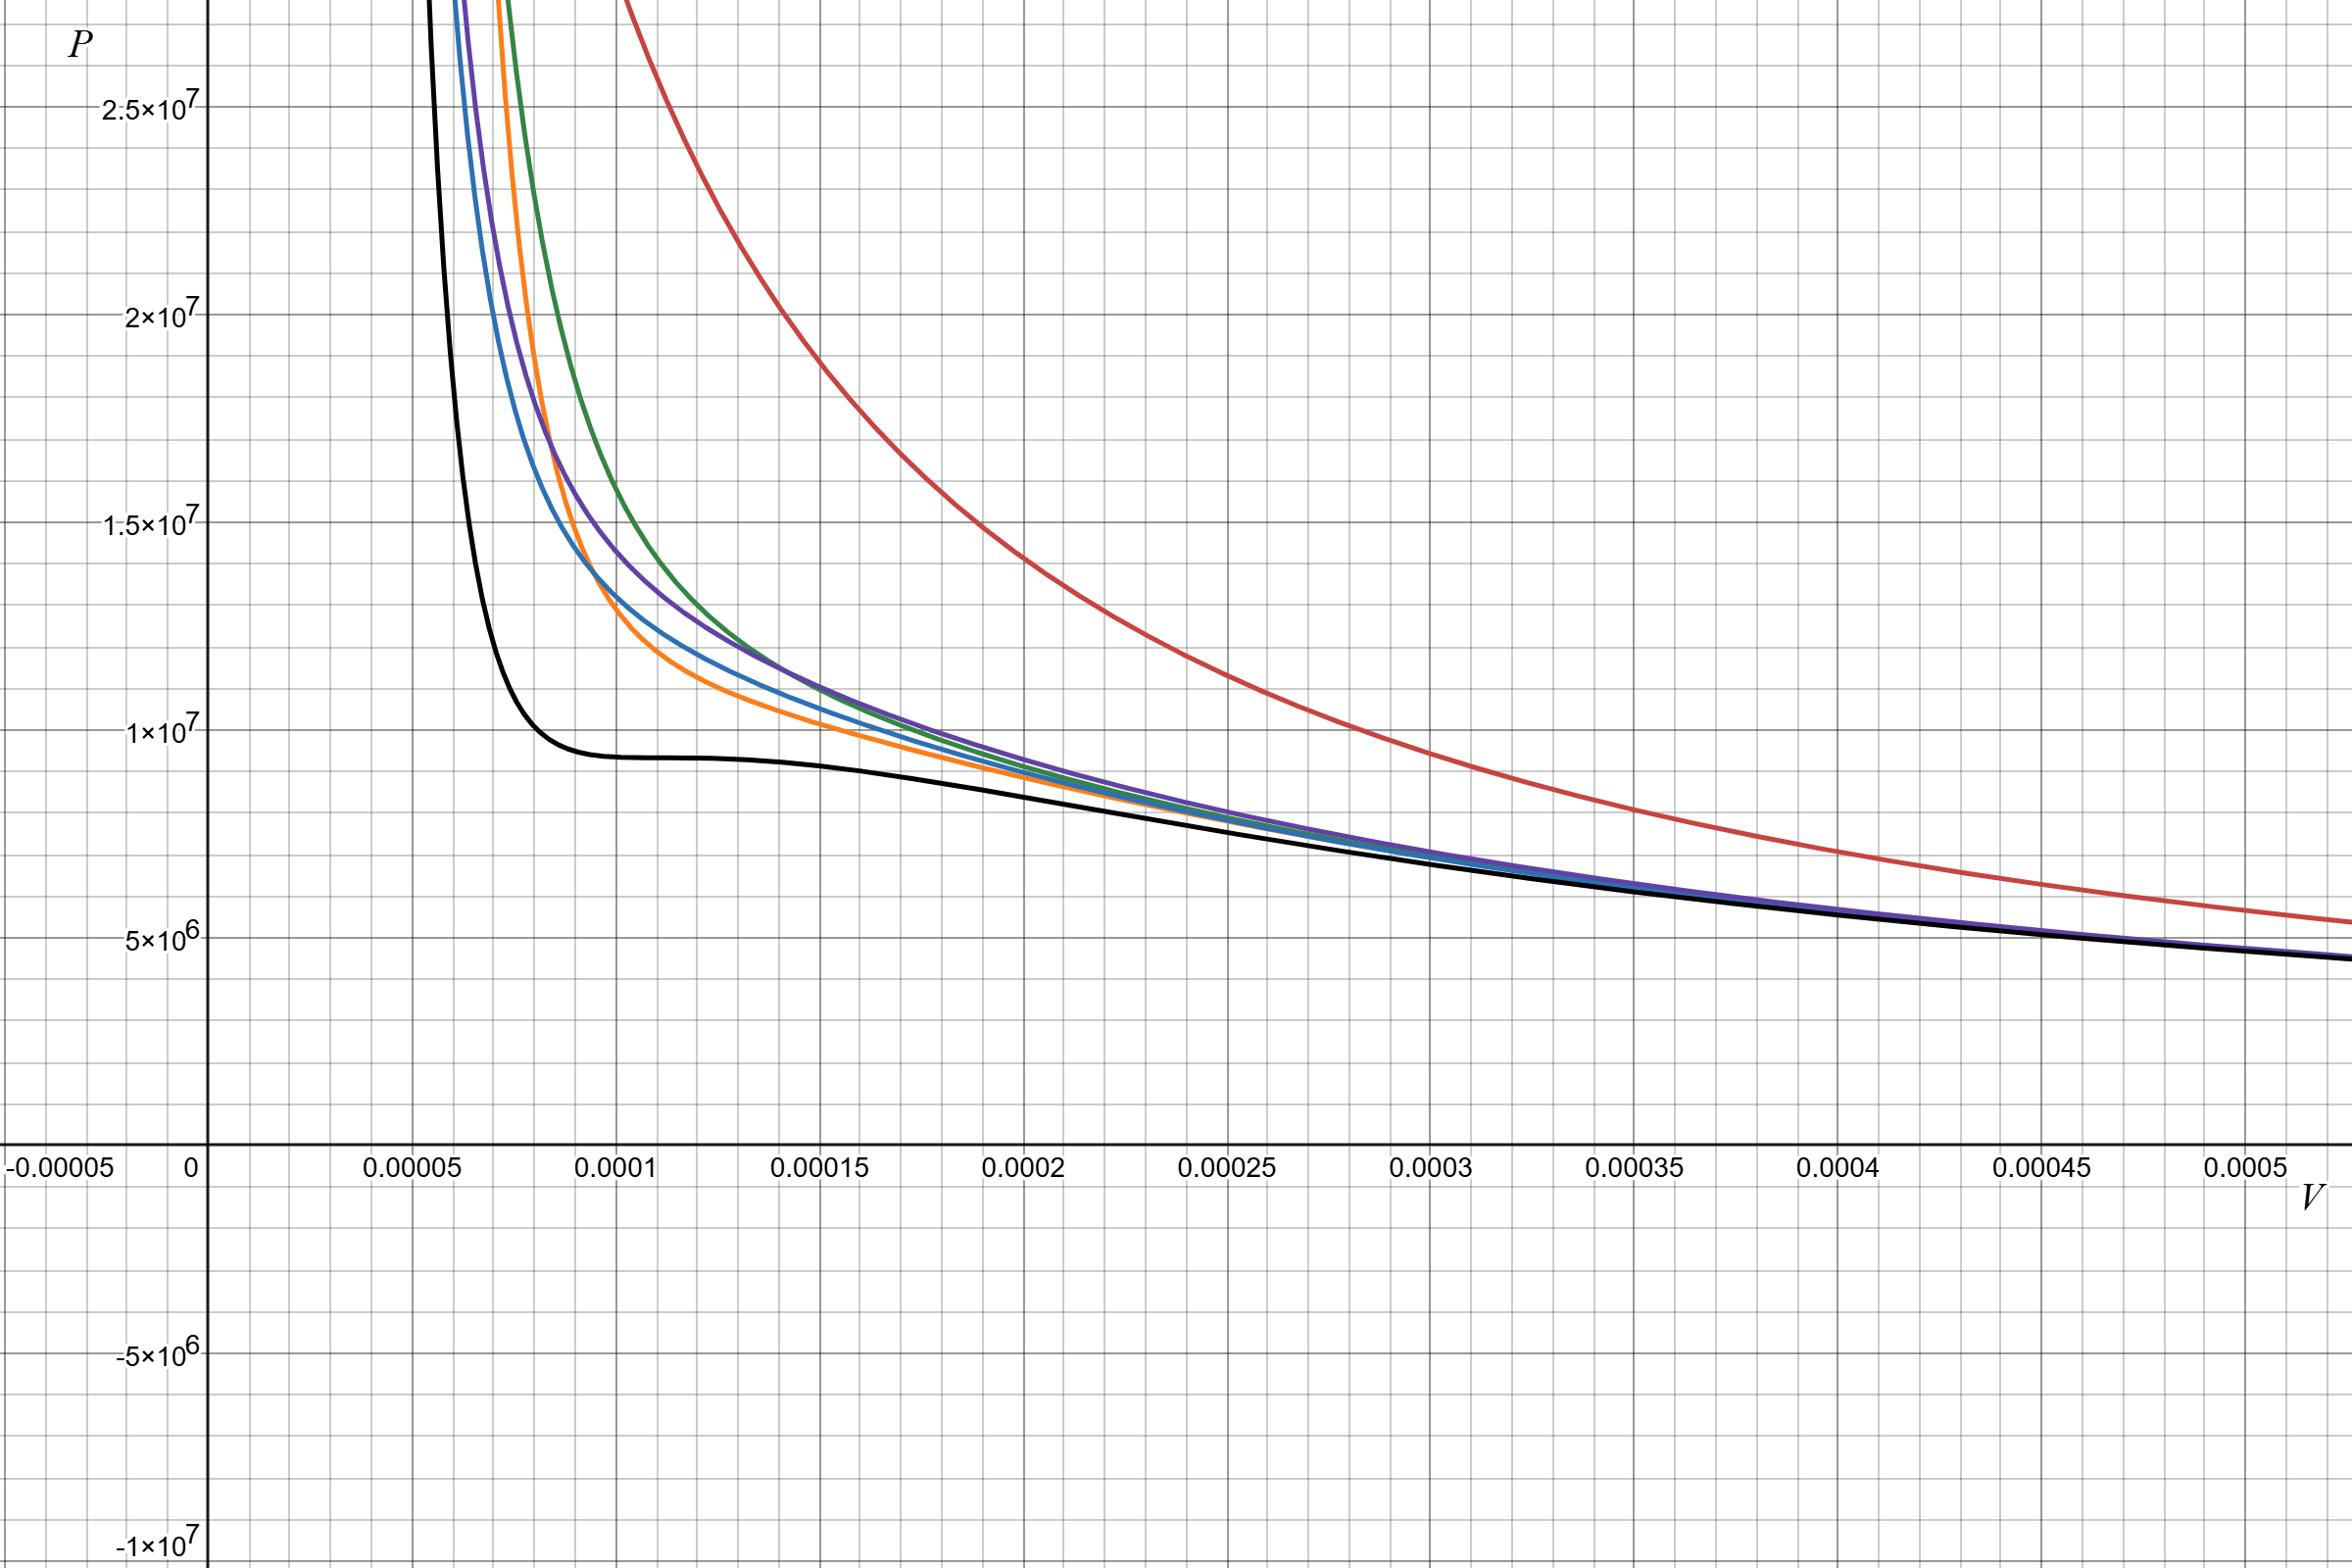
\includegraphics[width=\linewidth]{Graphics/CO2/340_1.png}
        \caption{\label{fig:clausius_1}График 15. $P-V$ сравнительное построение графиков уравнений состояния углекислого газа $CO_2$, $T = 340.1 \ \text{K}$}
    \end{minipage}
\end{figure}

\begin{figure}[h!]
    \centering
    \begin{minipage}{0.49\textwidth}
        \centering
        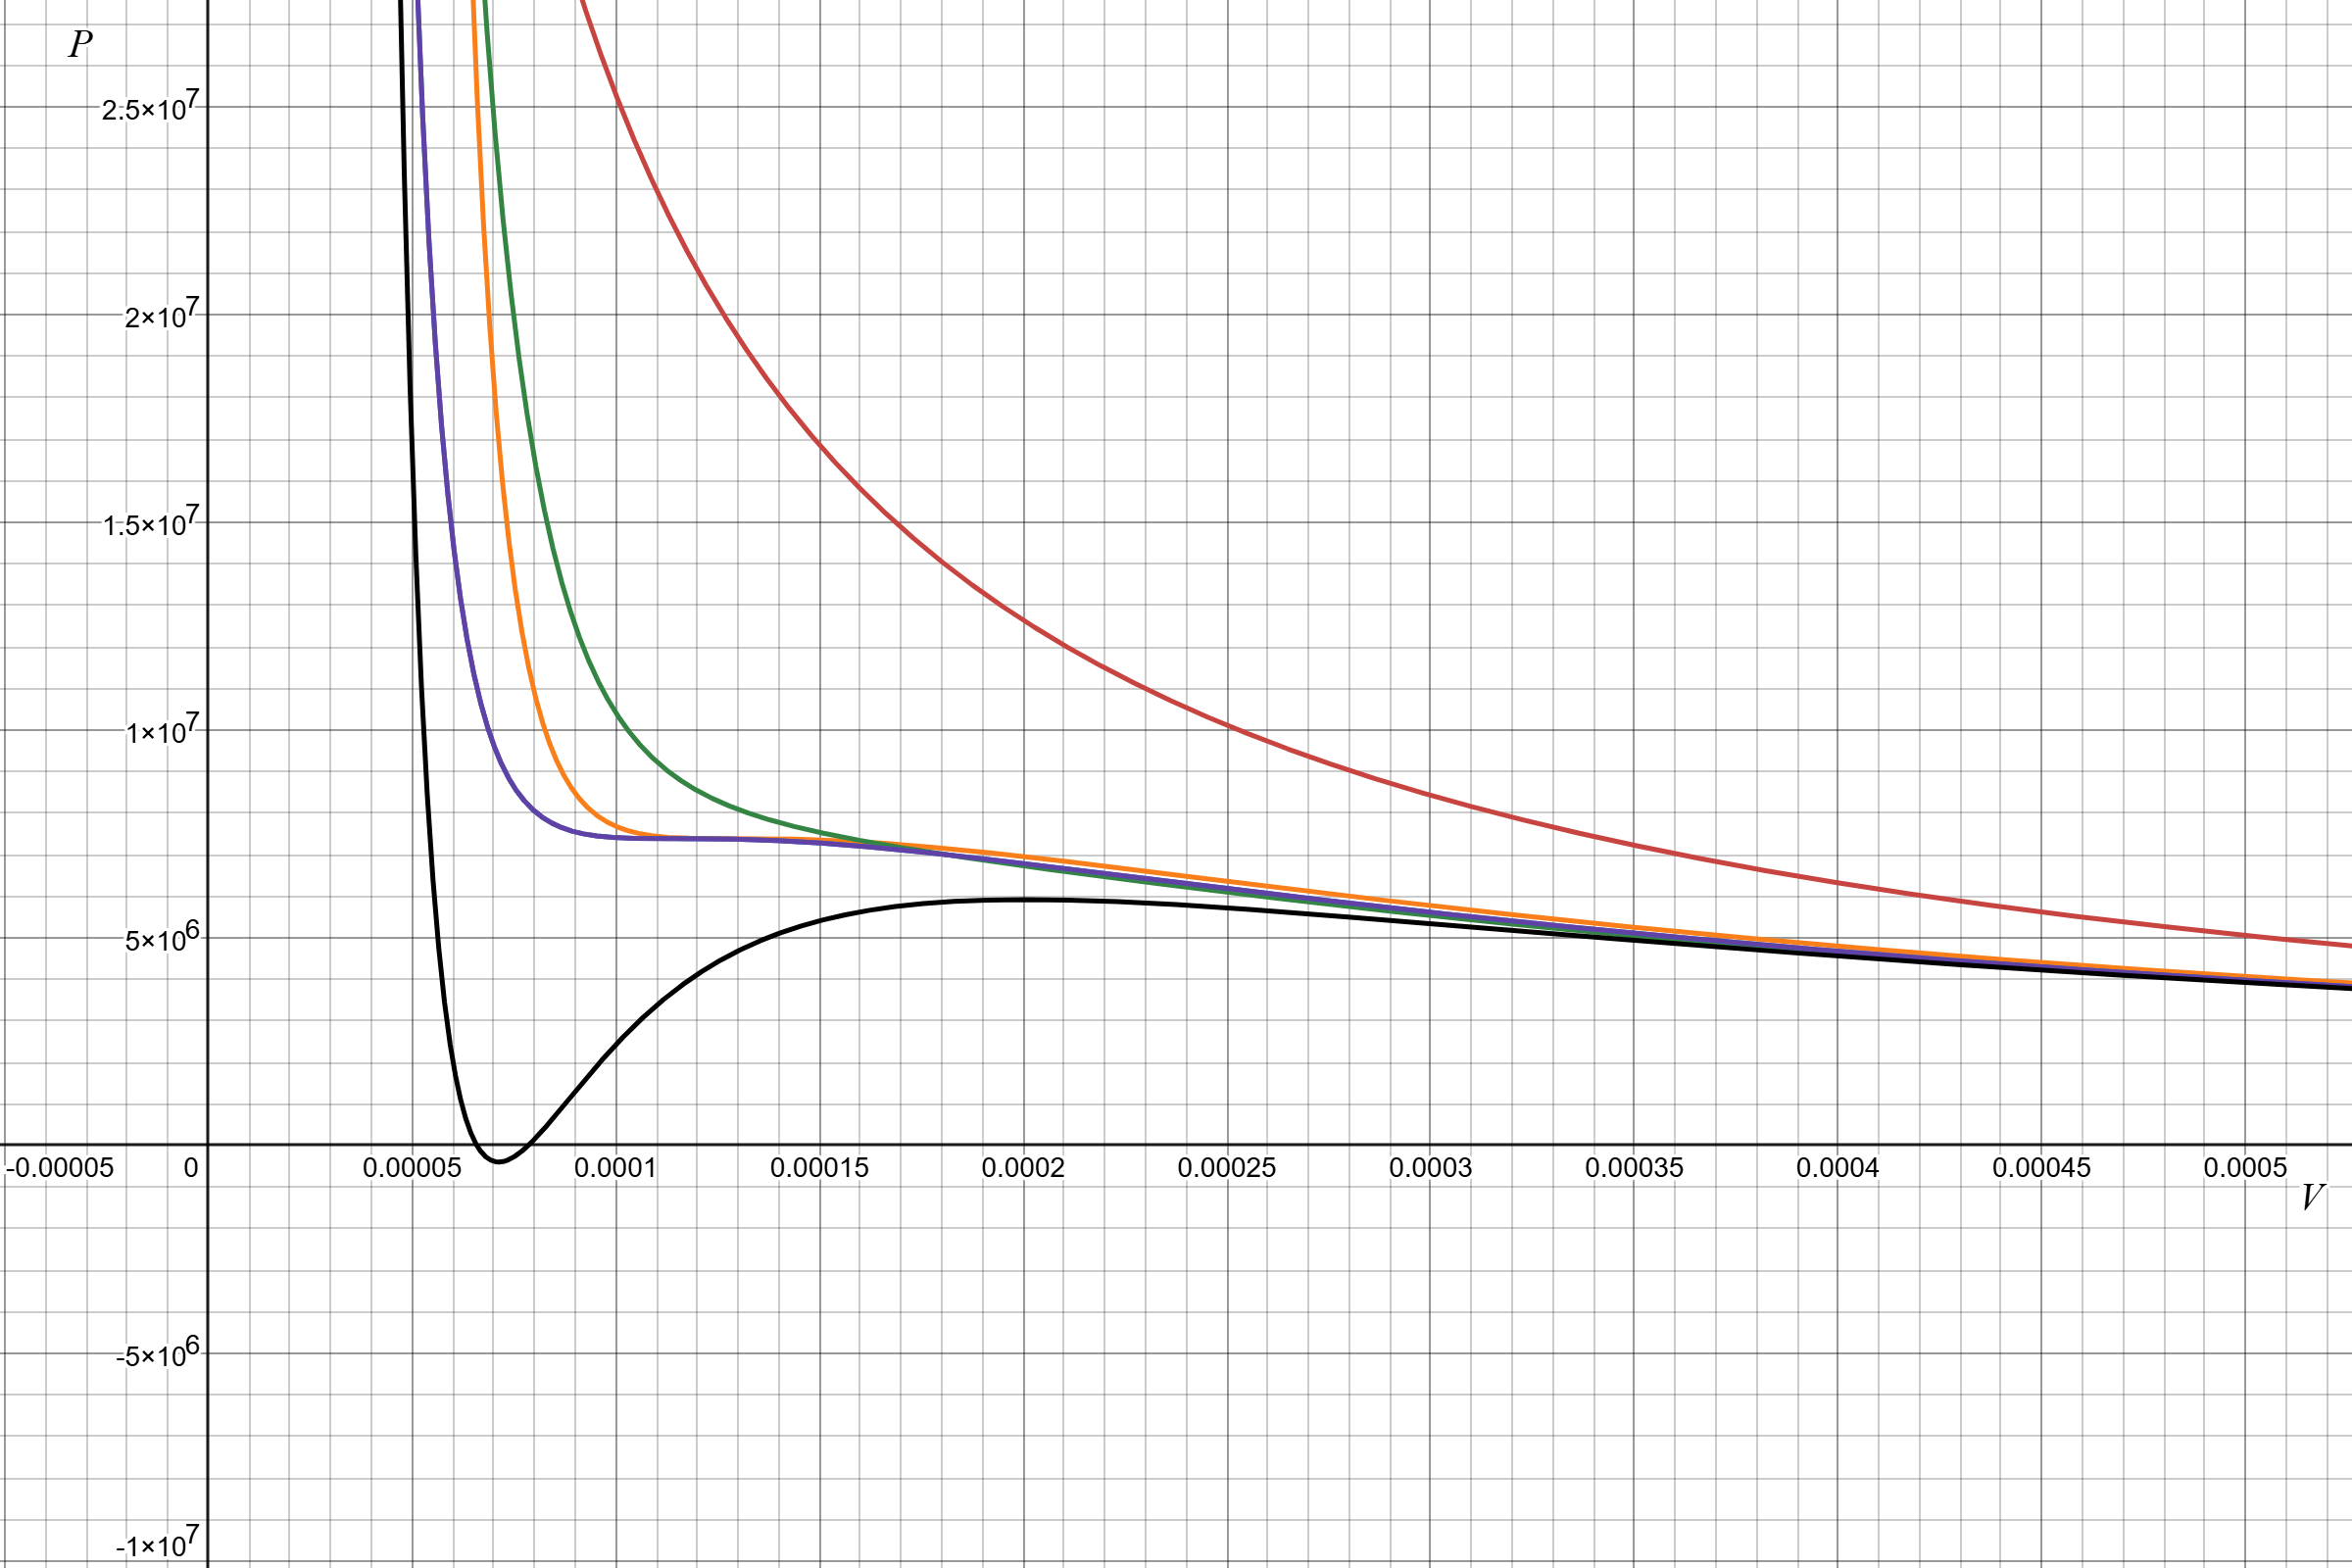
\includegraphics[width=\linewidth]{Graphics/CO2/304_15.png}
        \caption{\label{fig:clausius_1}График 16. $P-V$ сравнительное построение графиков уравнений состояния углекислого газа $CO_2$, $T = 304.15 \ \text{K}$}
    \end{minipage}
    \hfill
    \begin{minipage}{0.49\textwidth}
        \centering
        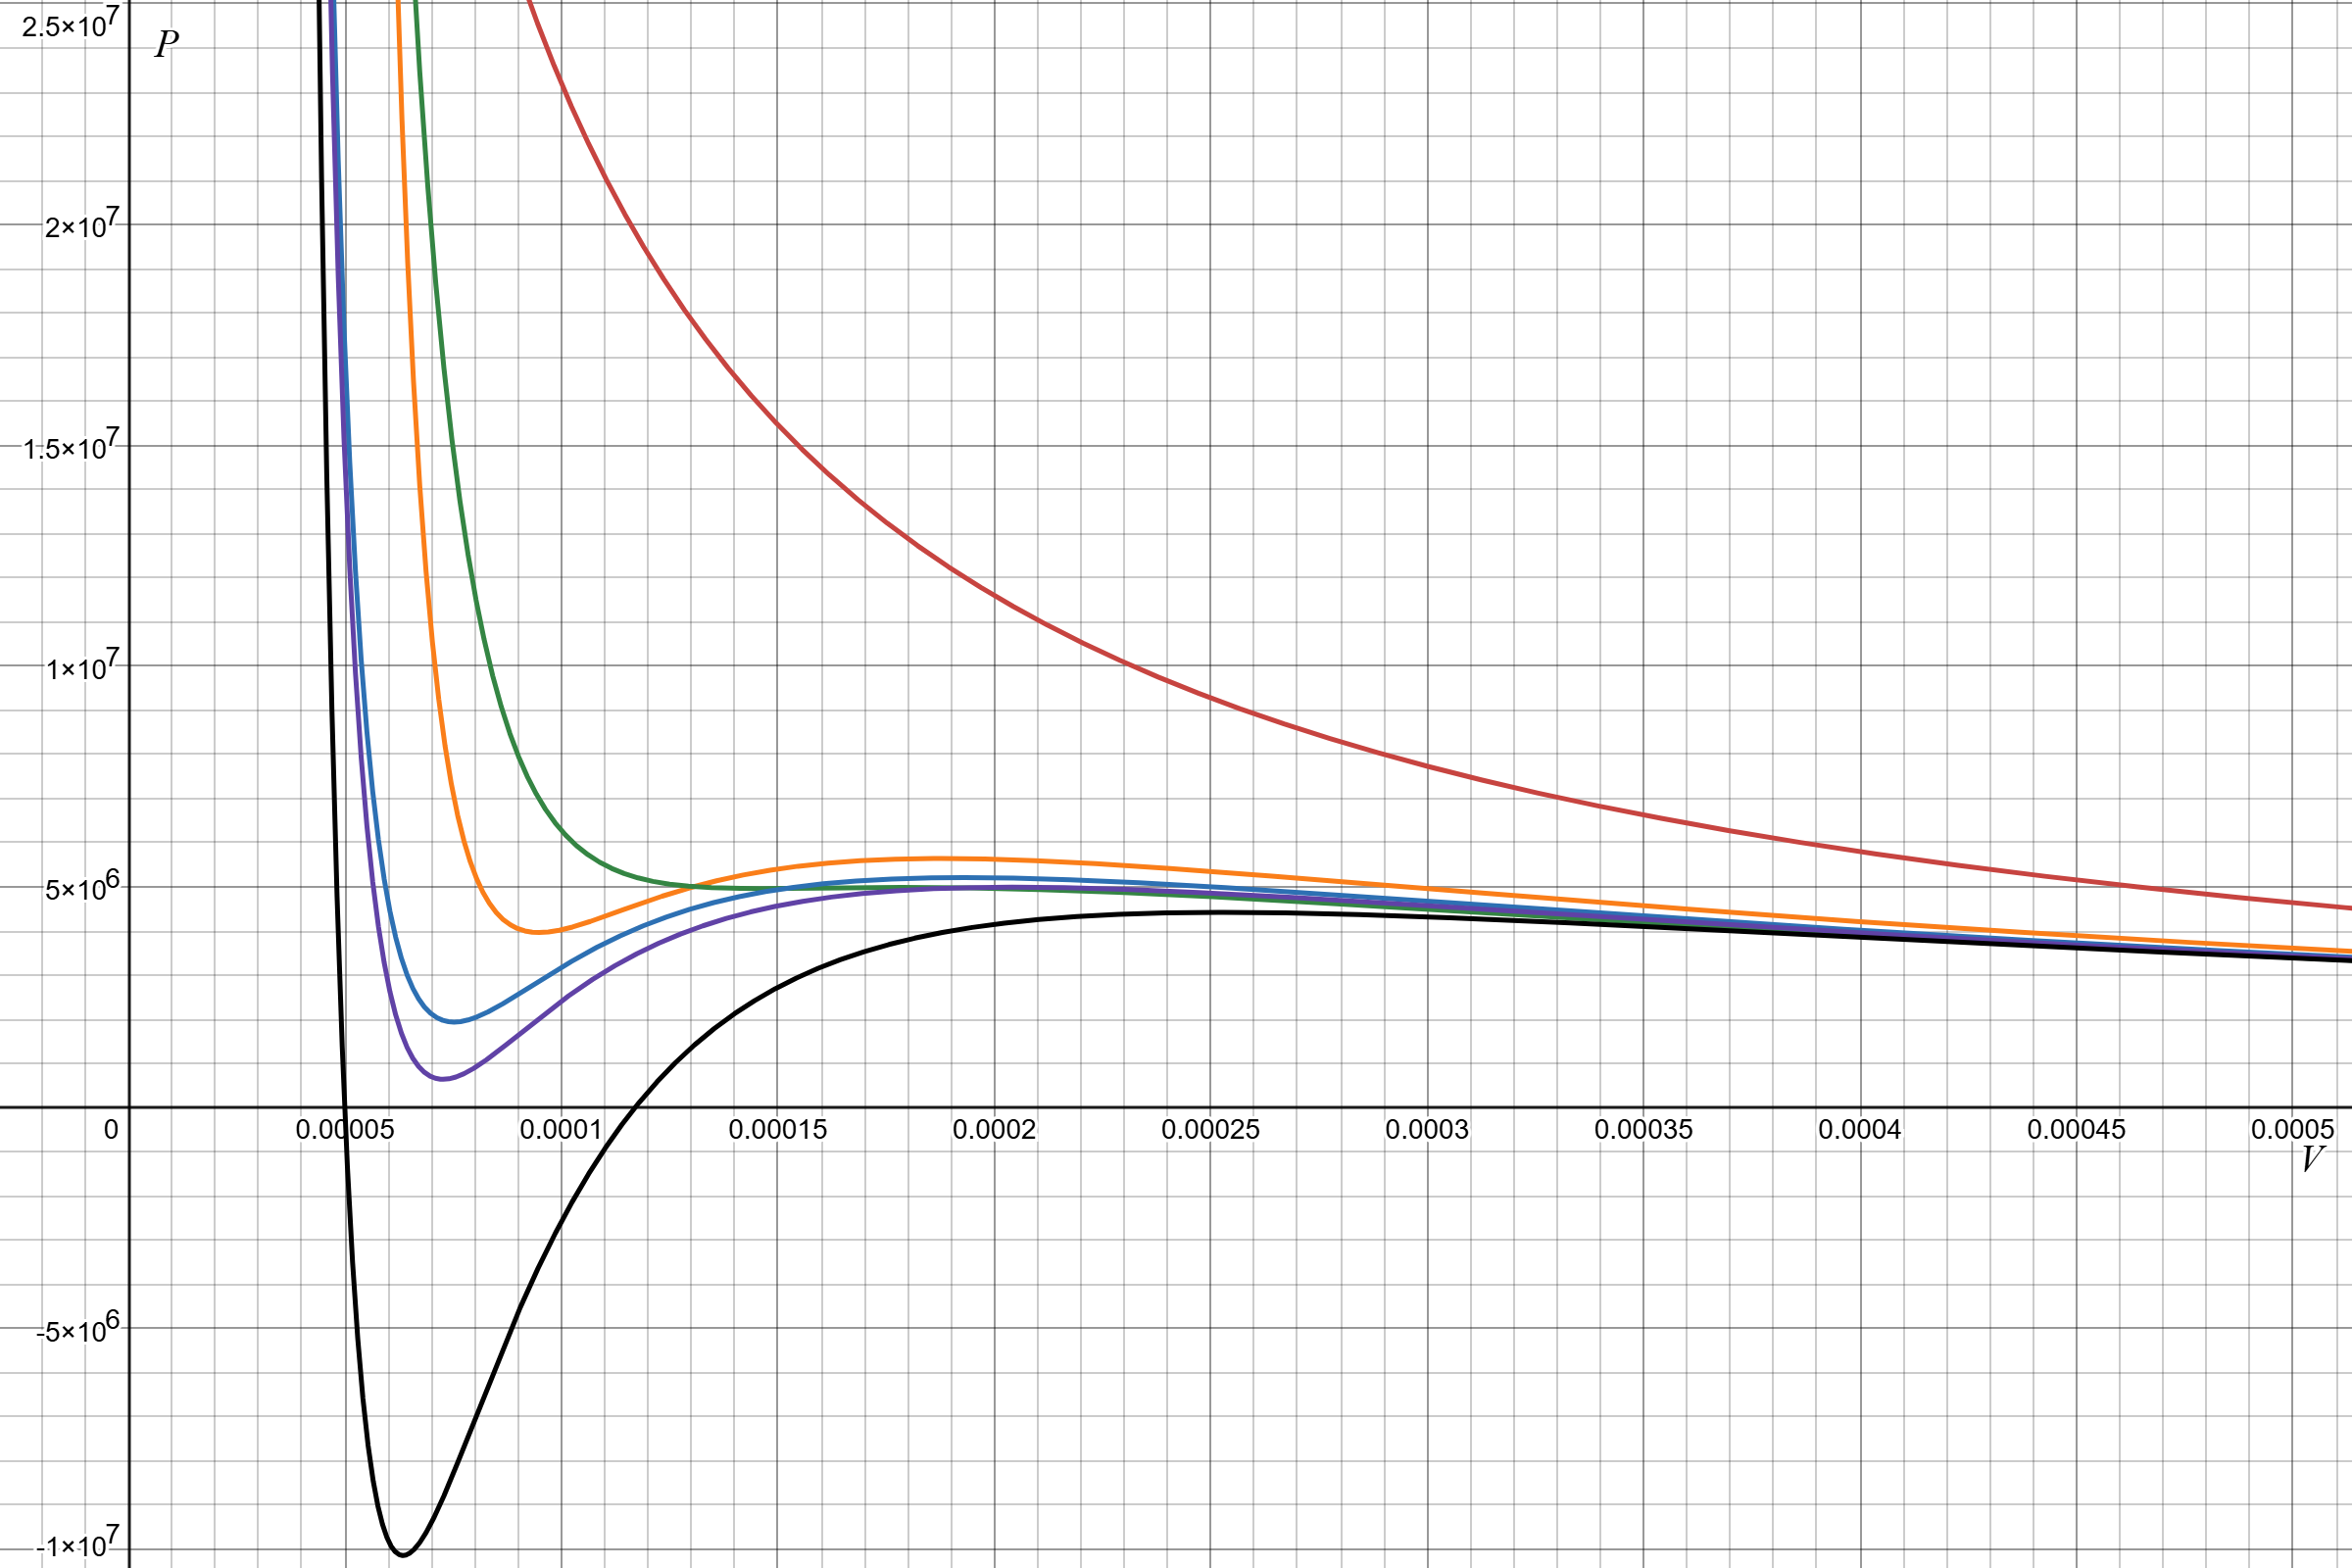
\includegraphics[width=\linewidth]{Graphics/CO2/279.png}
        \caption{\label{fig:clausius_1}График 17. $P-V$ сравнительное построение графиков уравнений состояния углекислого газа $CO_2$, $T = 279 \ \text{K}$}
    \end{minipage}
\end{figure}
\clearpage
\begin{figure}[h!]
    \centering
    \begin{minipage}{0.49\textwidth}
        \centering
        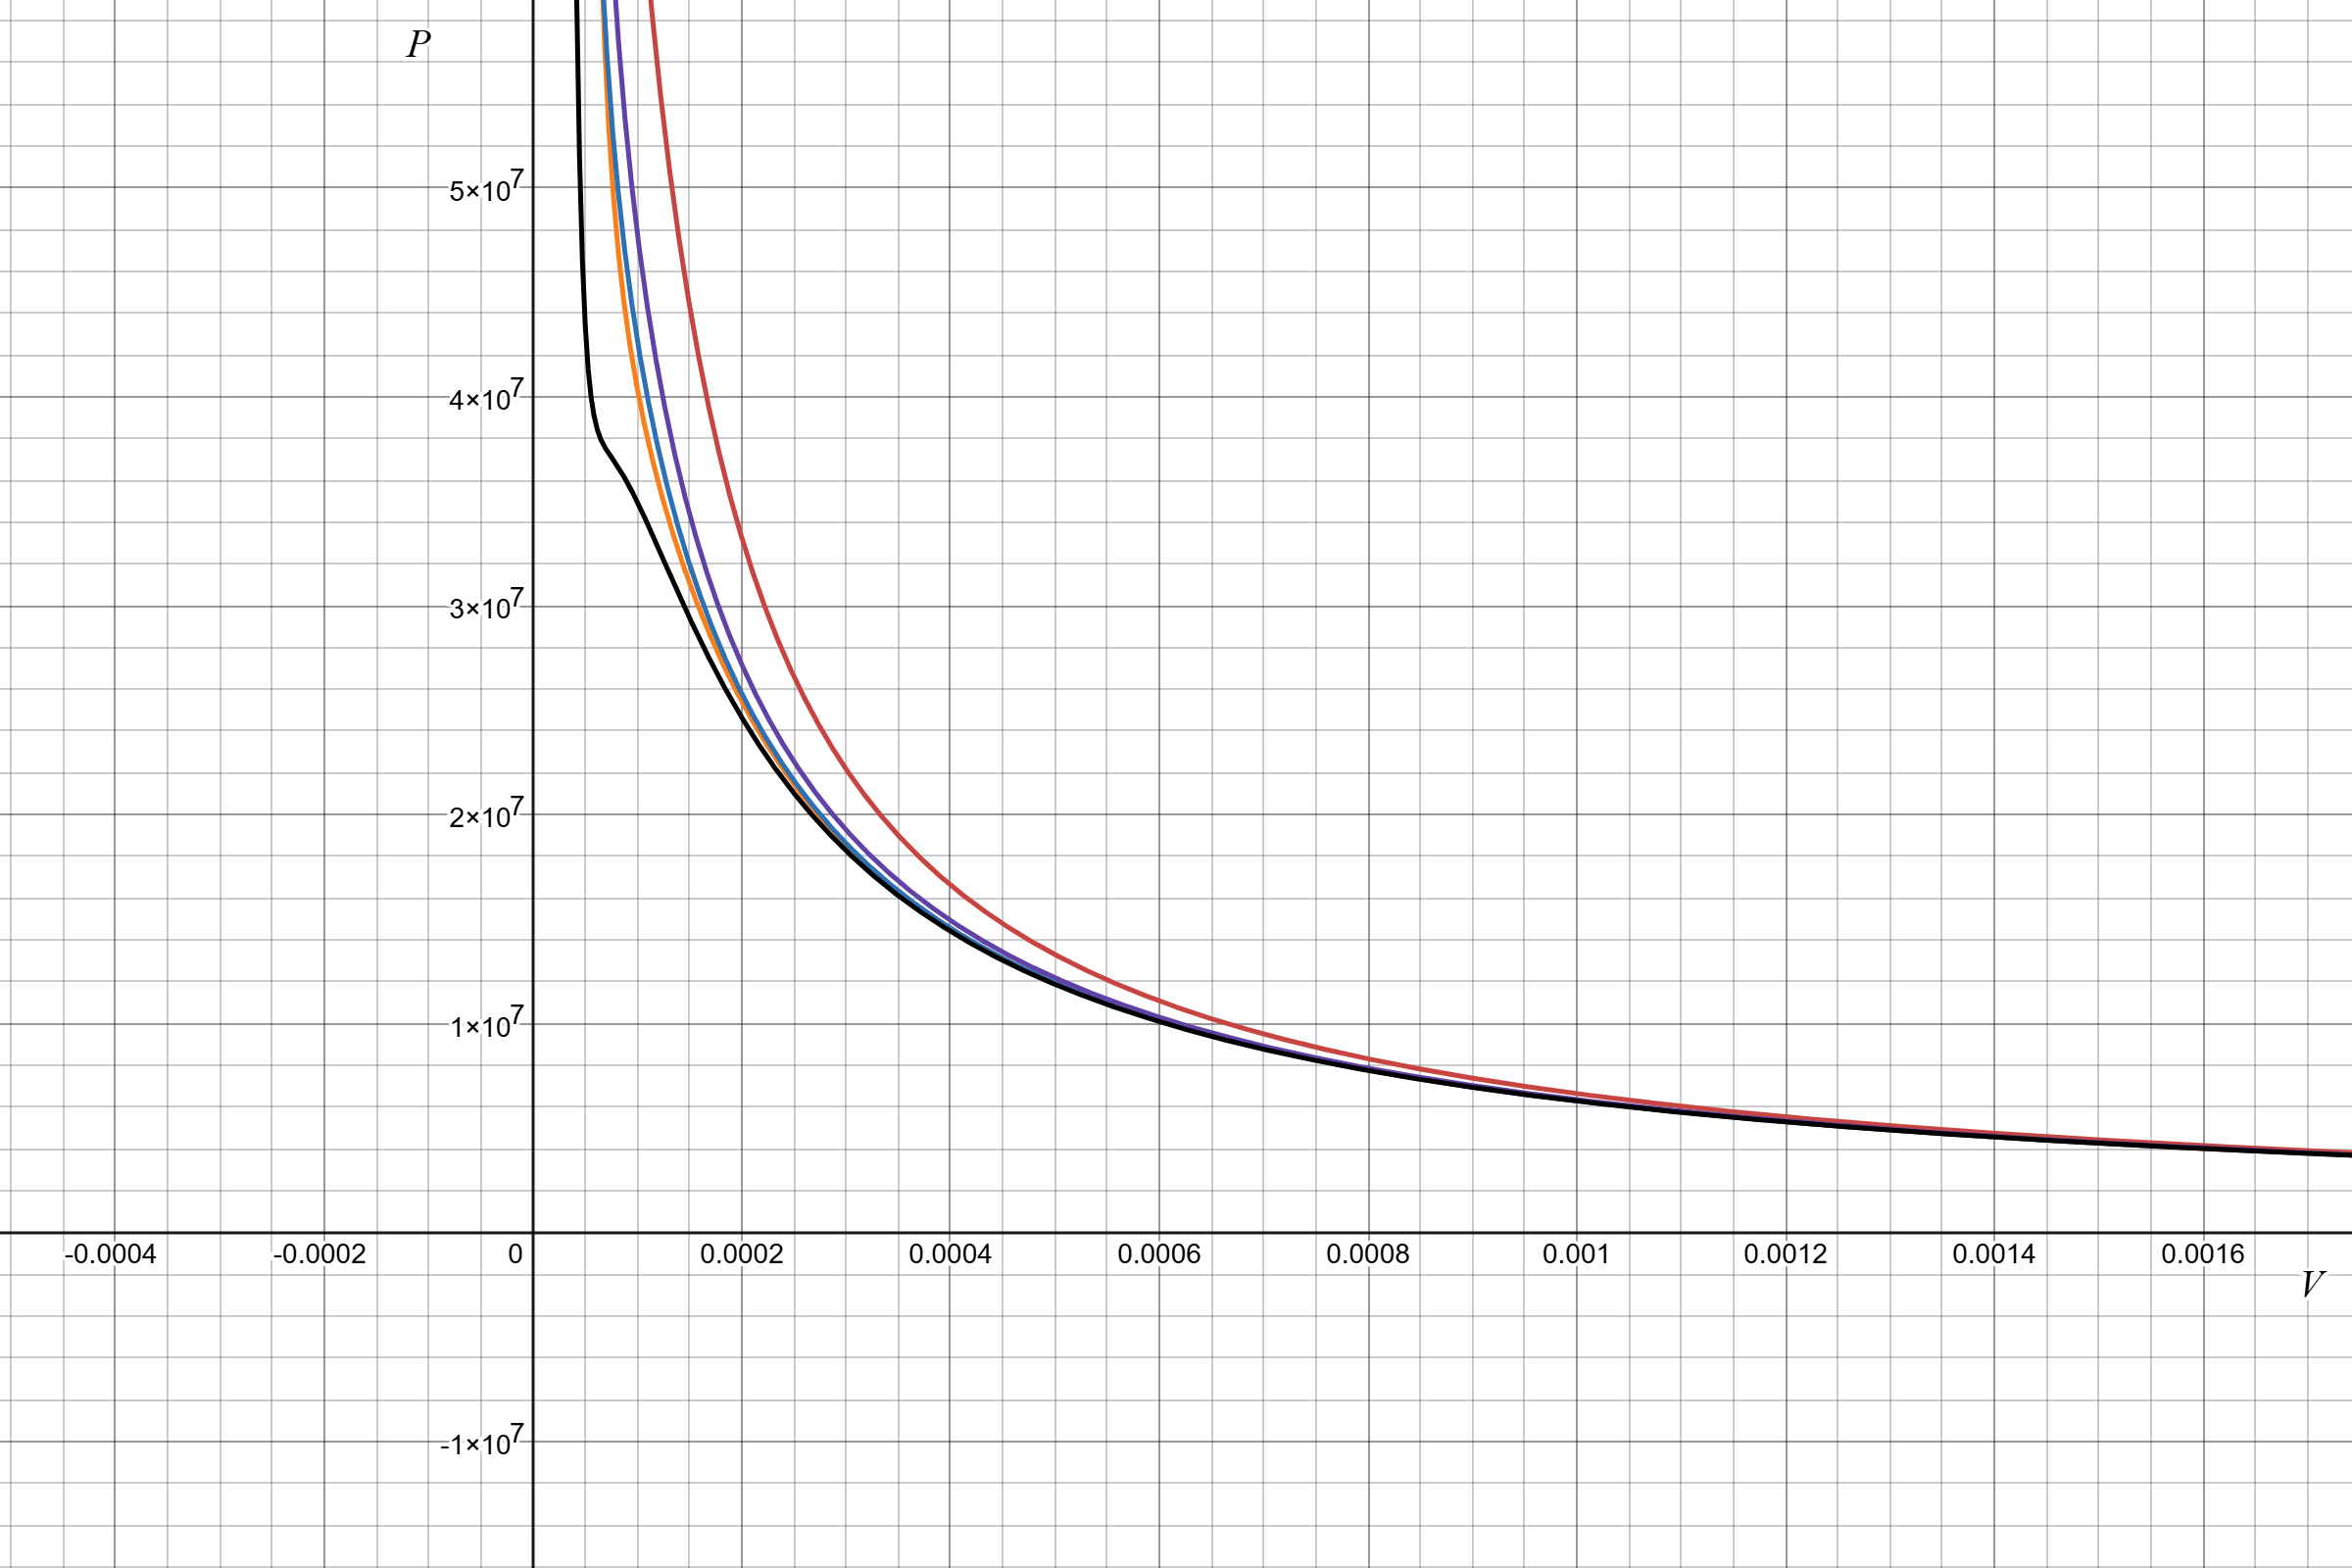
\includegraphics[width=\linewidth]{Graphics/H2O/800.png}
        \caption{\label{fig:clausius_1}График 18. $P-V$ сравнительное построение графиков уравнений состояния воды $H_2O$, $T = 800 \ \text{K}$}
    \end{minipage}
    \hfill
    \begin{minipage}{0.49\textwidth}
        \centering
        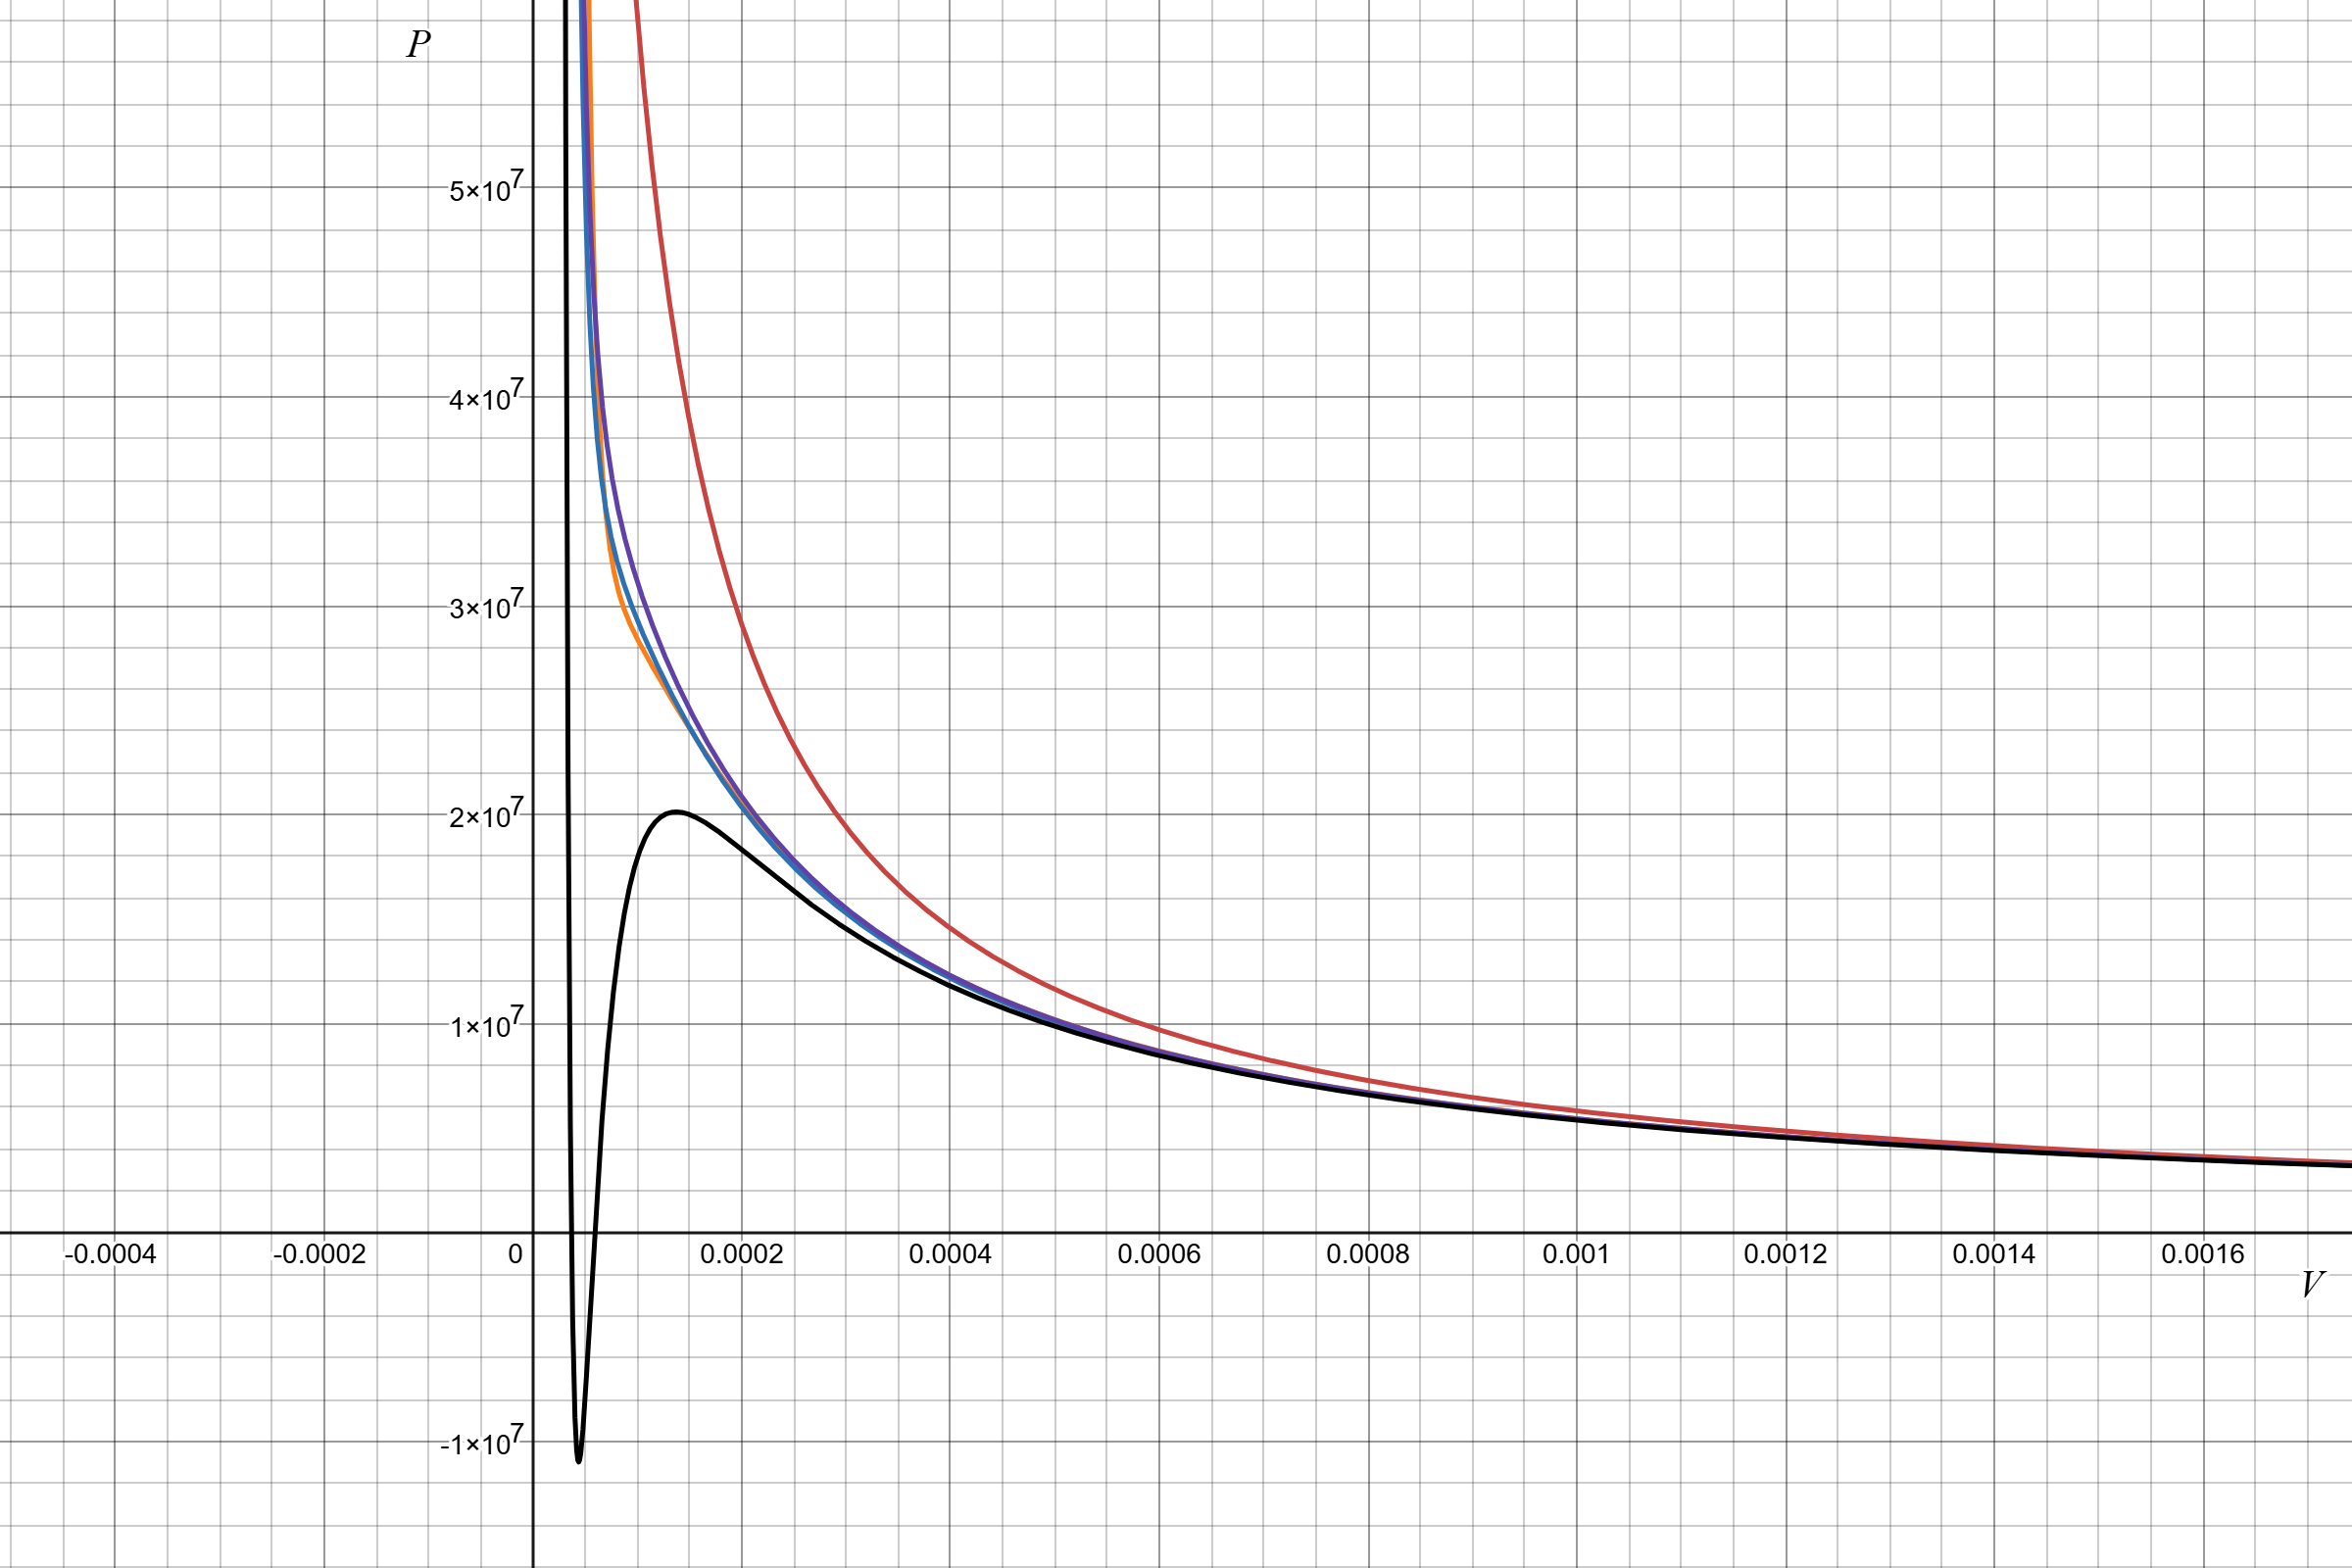
\includegraphics[width=\linewidth]{Graphics/H2O/700.png}
        \caption{\label{fig:clausius_1}График 19. $P-V$ сравнительное построение графиков уравнений состояния воды $H_2O$, $T = 700 \ \text{K}$}
    \end{minipage}
\end{figure}

\begin{figure}[h!]
    \centering
    \begin{minipage}{0.49\textwidth}
        \centering
        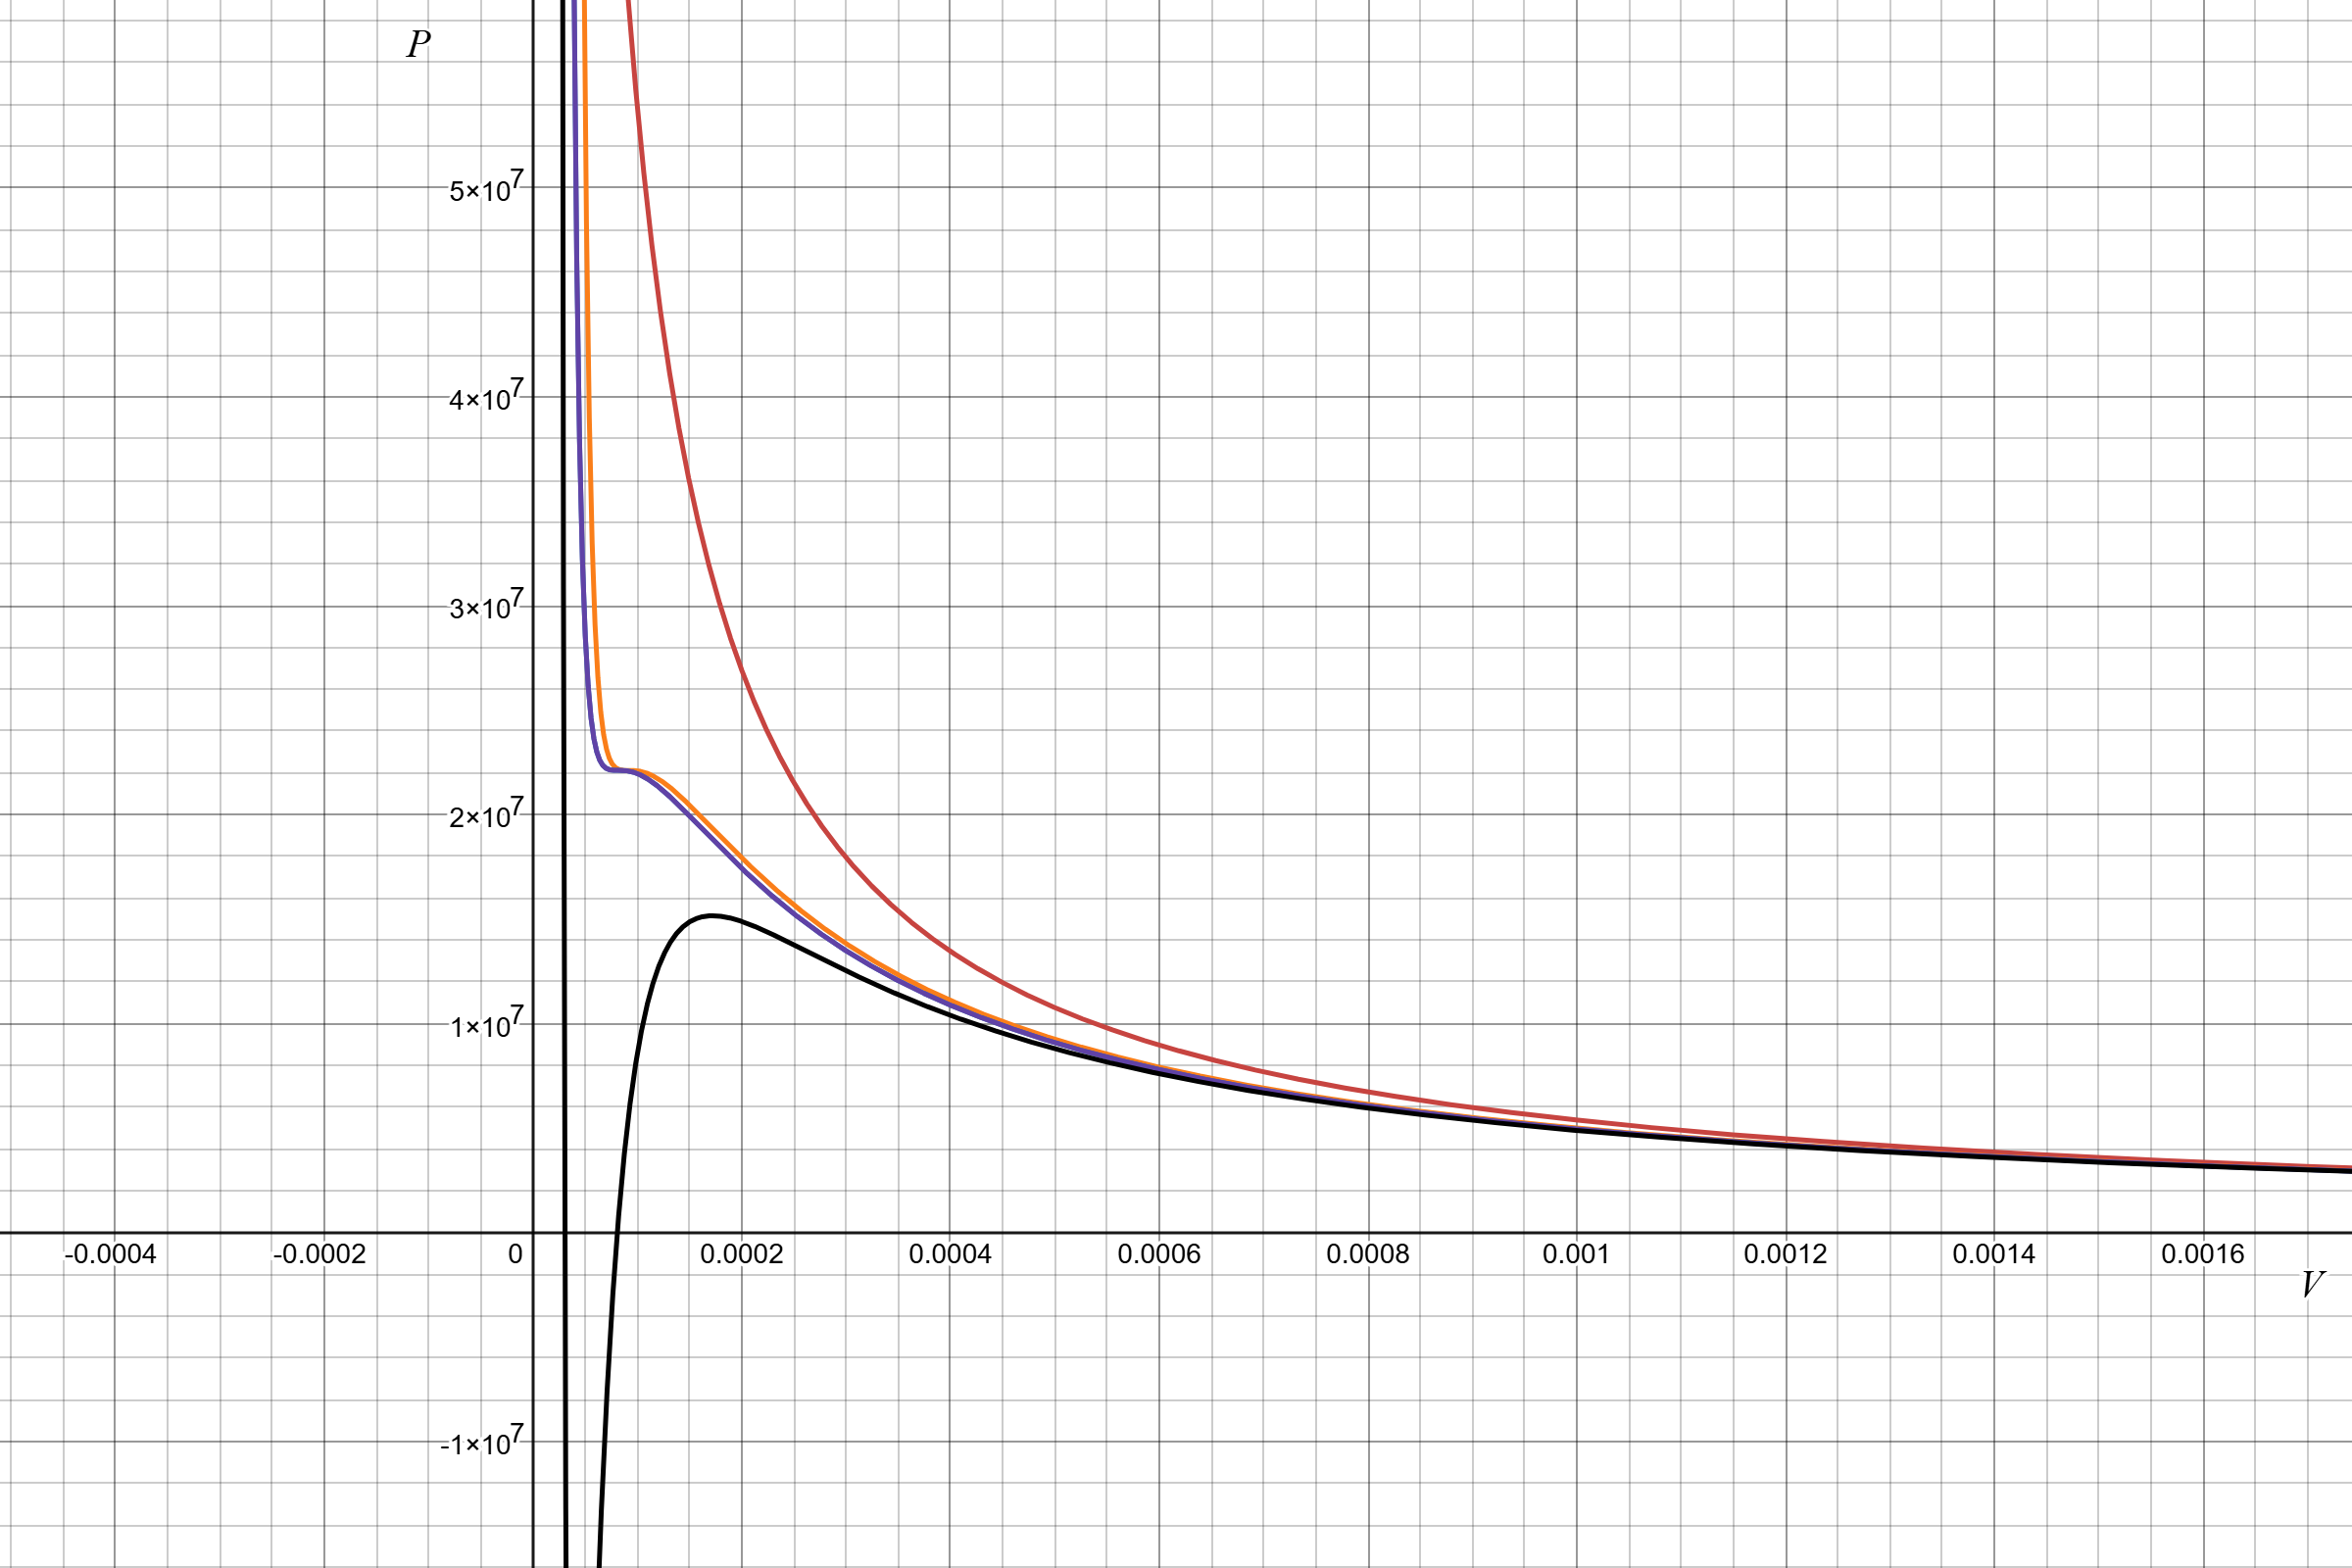
\includegraphics[width=\linewidth]{Graphics/H2O/647_3.png}
        \caption{\label{fig:clausius_1}График 20. $P-V$ сравнительное построение графиков уравнений состояния воды $H_2O$, $T = 647.3 \ \text{K}$}
    \end{minipage}
    \hfill
    \begin{minipage}{0.49\textwidth}
        \centering
        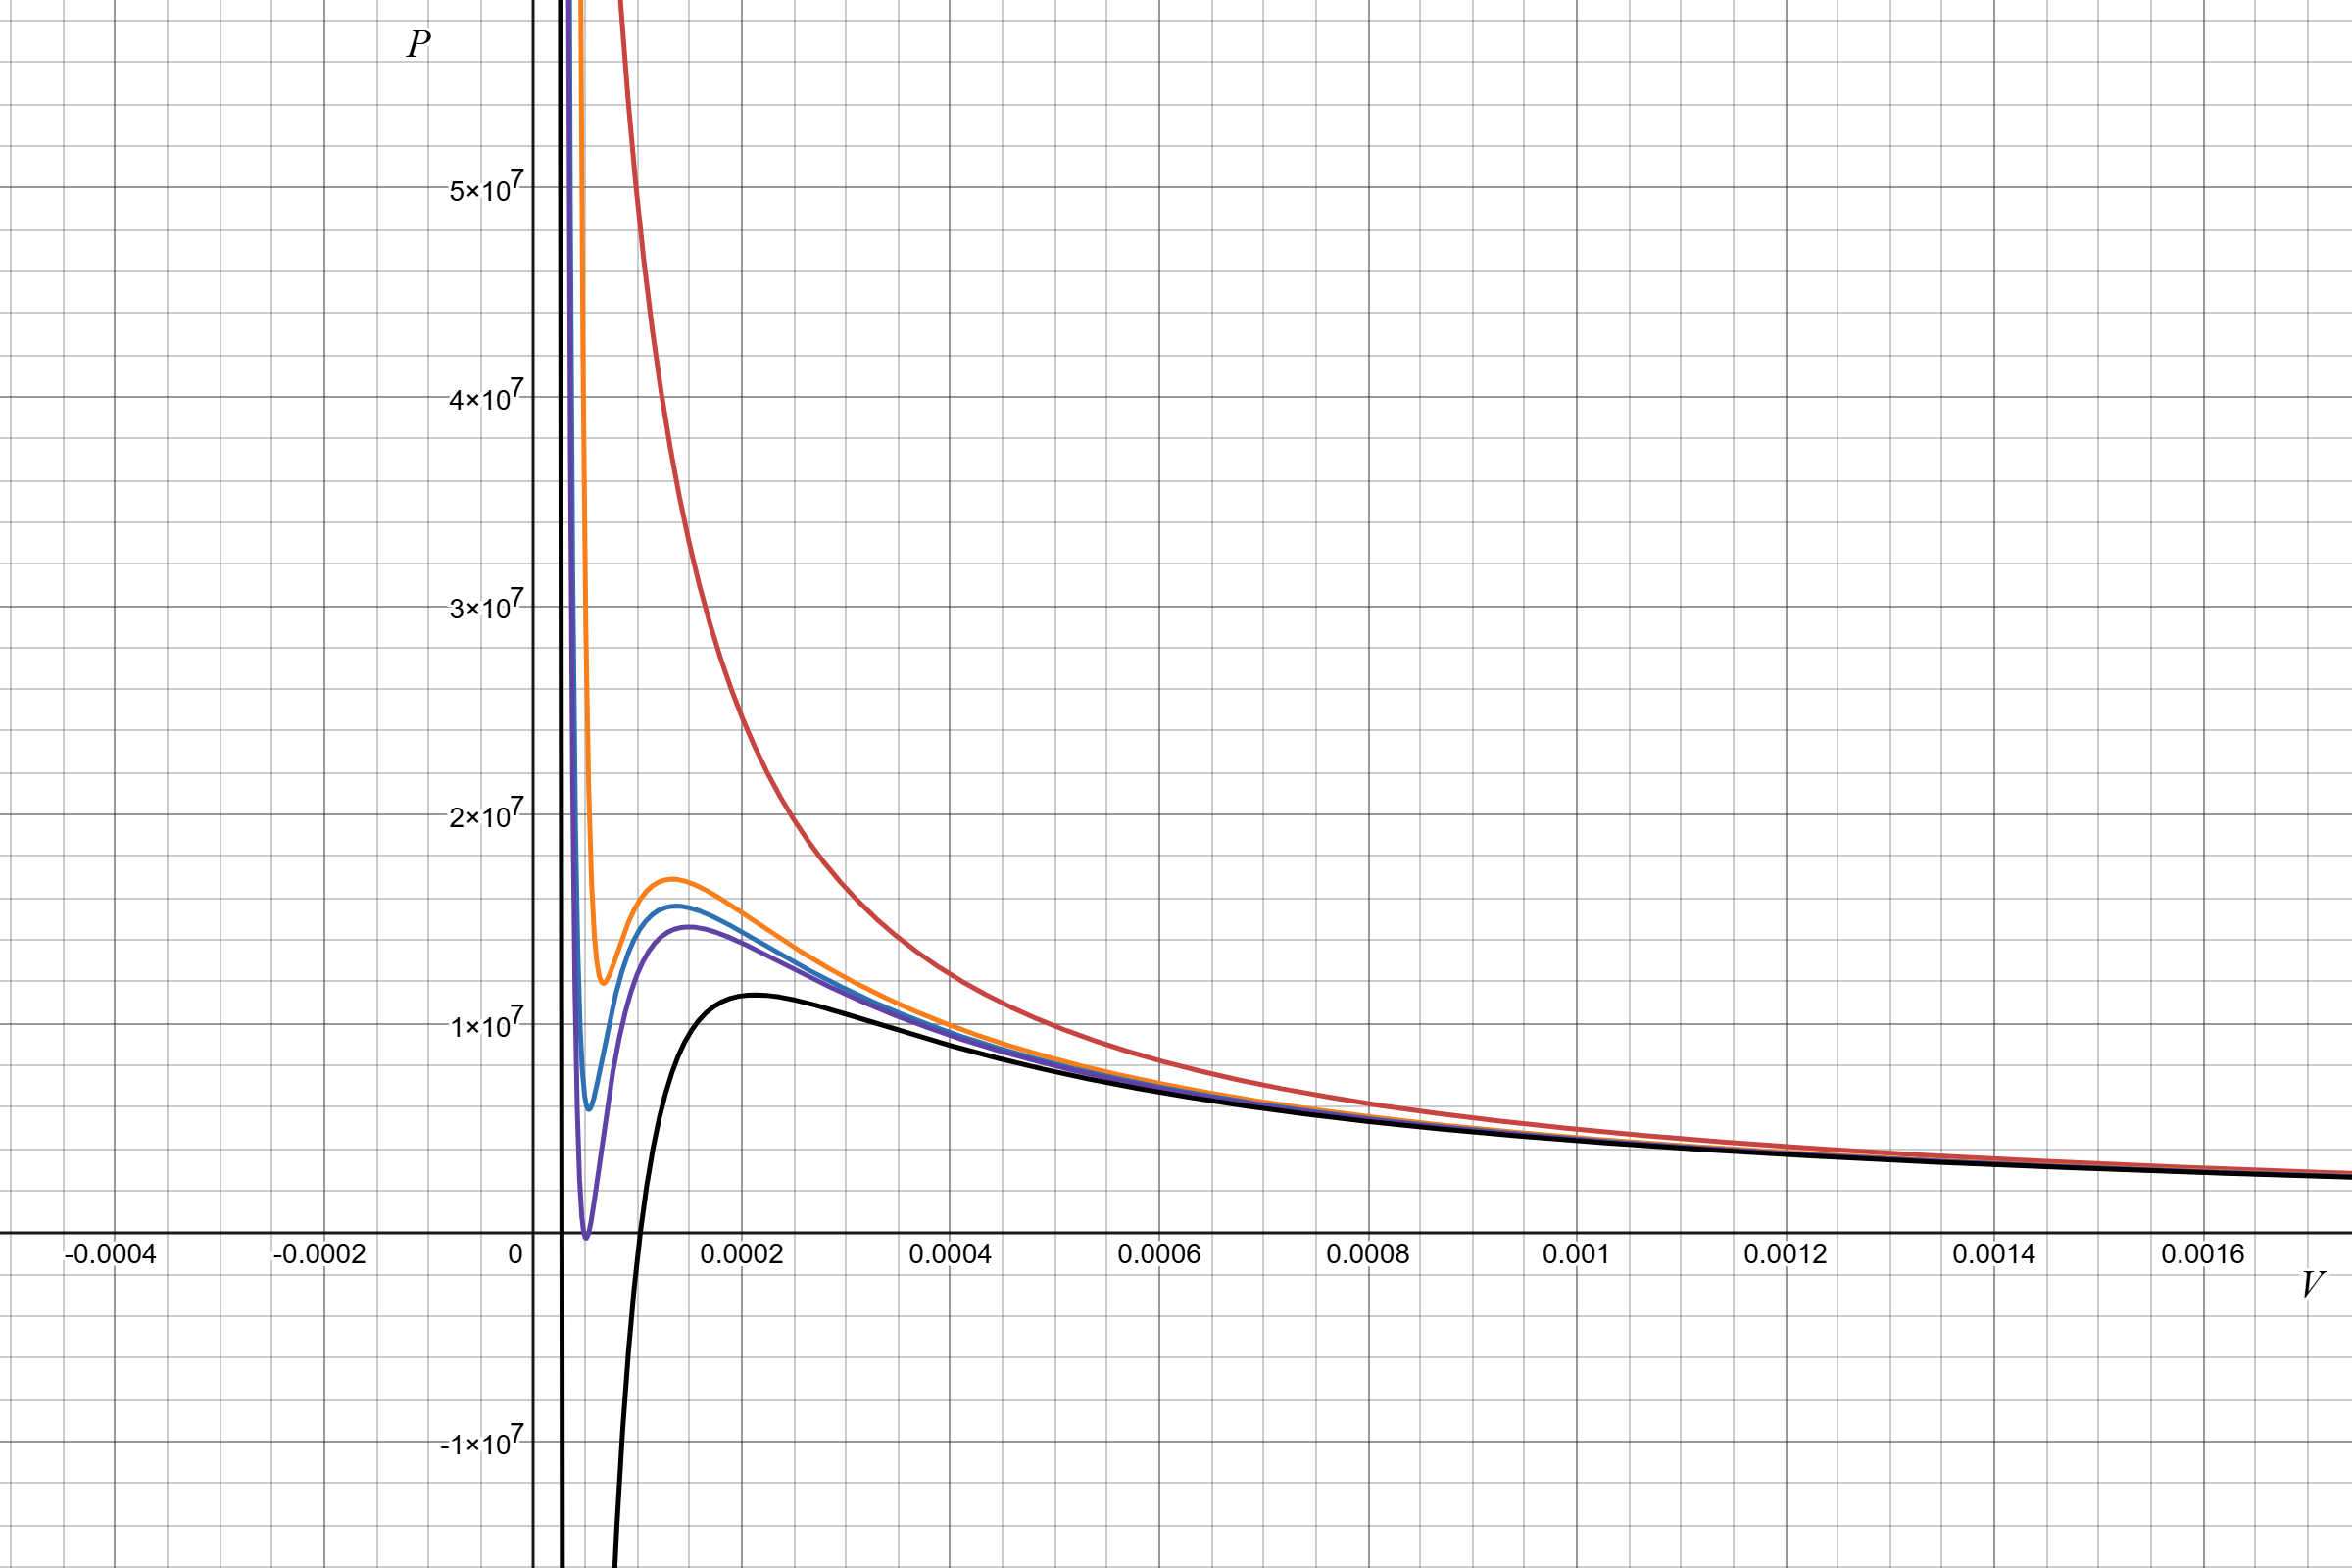
\includegraphics[width=\linewidth]{Graphics/H2O/594.png}
        \caption{\label{fig:clausius_1}График 21. $P-V$ сравнительное построение графиков уравнений состояния воды $H_2O$, $T = 594 \ \text{K}$}
    \end{minipage}
\end{figure}

Как мы видим, уравнения PR и Битти-Бриджмена не точно отражают действительные критические температуры. В первом случае из-за нетабличных коэффициентов, во втором из-а простоты уравнения. Лучше всего критическую точку описывают уравнения Ван-дер-Ваальса, RK и SRK.

\section{Выводы}
В данной работе мы разобрали основные исторические этапы развития уравнения состояния вещества: от Менделеева-Клапейрона, до самых современных. Сравнили некоторые из них, построив графики. Попытались обосновать физически модели уравнений, привели для некоторых строгие доказательства.

\clearpage
\section{Приложение}
\subsection{Конспект физического обоснования уравнения Дитеричи}
Источник: Д.В. Сивухин, Термодинамика и молекулярная физика, Том II.

\begin{enumerate}
\item Будем считать, что силы отталкивания возникают только при непосредственном контакте молекул со стенкой. Молекулы пристеночного слоя подвергаются действию результирующей силы, направленной внутрь газа. Вследствие этого концентрация молекул в пристеночном слое должна убывать при приближении к стенке в соответсвие с формулой Больцмана:
\begin{equation}
      n = n_{\infty}e^{-\frac{U(x)}{kT}}, \label{eq:Dieterici0}
\end{equation}
где $U(x)$ -- потенциальная энергия молекулы. Она максимальна у самой стенки и быстро убывает с ростом $x$. Ее значение на бесконечности $U_{\infty}$(на расстоянии больше радиуса сферы молекулярного действия) условимся считать равным нулю. Тогда давление на стенку определяется как:
\begin{equation}
      P = n_0kT = n_{\infty}kTe^{-\frac{U_0}{kT}}, \label{eq:myeq0}
\end{equation}
где $U_0$ -- потенциальная энергия молекулы у стенки сосуда.
\item Сила притяжения, действующая на пристеночную молекулу, а с ней и потенциальная энергия $U_0$, пропорциональны концентрации молекул газа $n_{\infty} = \frac{N}{V}$. Поэтому можно написать $U_0 = \alpha n_{\infty}$, где $\alpha$ -- постоянная для рассматриваемого газа величина. Если ввести еще одну постоянную $a = \alpha N^2$, то:
\begin{equation}
      U_0 = \frac{a}{NV}.
\end{equation}
подставим в \ref{eq:Dieterici0}:
\begin{equation}
      P = n_{\infty}kTe^{-\frac{U_0}{kT}} = \frac{RT}{V}e^{-\frac{a}{RVT}}.
\end{equation}
\item Введем ту же поправку на объем что и в уравнении Ван-дер-Ваальса и получим уравнение Дитеричи:
\begin{equation}
      P =  \frac{RT}{V-b}e^{-\frac{a}{RVT}}.
\end{equation}
\end{enumerate}

\subsection{Конспект физического обоснования уравнения Битти-Бриджмена}

Источник: \href{https://www.jstor.org/stable/20026205?searchText=Beattie\%2C+J.A.\%2C+Bridgeman\%2C+O.C.+\%22A+New+Equation+of+State+for+Fluids\%22&searchUri=\%2Faction\%2FdoBasicSearch\%3FQuery\%3DBeattie\%252C\%2BJ.A.\%252C\%2BBridgeman\%252C\%2BO.C.\%2B\%2522A\%2BNew\%2BEquation\%2Bof\%2BState\%2Bfor\%2BFluids\%2522\%26so\%3Drel&ab_segments=0\%2Fbasic_phrase_search\%2Fcontrol&refreqid=fastly-default\%3A3700c3db53f265ea23b574296ef458ee&seq=1}{Beattie, J.A., Bridgeman, O.C. "A New Equation of State for Fluids"}
\begin{enumerate}
\item Основное предположение: давление реального газа можно представить как разность двух компонент:
\begin{equation}
      P = P_{\text{кин}} - P_{\text{ког}}, \label{eq:myeq0}
\end{equation}
где:\\
- $P_{\text{кин}}$ -- кинетическое давление, обусловленное движением молекул,\\
- $P_{\text{ког}}$ -- когезионное давление, обусловлено межмолекулярными силами притяжения.\\
В идеальном газе ($P_{\text{ког}} = 0$) давление определяется только ударами молекул о стенки сосуда. В реальном газе межмолекулярные силы создают дополнительное "внутреннее" поле, которое уменьшает наблюдаемое давление на границе.
\item \textbf{Кинетическое давление}.\\ 
Для идеального газа (без взаимодействий и размера молекул):
\begin{equation}
      P_{\text{кин}} = \frac{RT}{V}.
\end{equation}
В реальном газе молекулы "отражаются" друг от друга из-за сил притяжения/отталкивания. Это увеличивает передачу импульса. Вводится коэффициент отражения $r$:
\begin{equation}
      P_{\text{кин}} = \frac{RT}{V}(1 + r). \label{eq:myeq1}
\end{equation}
Если плотность газа мала, так что молекулы действуют независимо как отражатели, отраженная доля пропорциональна плотности, и, следовательно, $r = \rho B$, так что уравнение \ref{eq:myeq1} принимает вид:
\begin{equation}
P_{\text{кин}} = \frac{RT}{V^2}(V + B). \label{eq:myeq2}
\end{equation}
Это выражение было впервые выведено Лоренцом из вириала Клау. Если плотность такова, что это простое предположение о независимом отражении недействительно, и отражательная способность на молекулу интерферирует с окружающими ее объектами, то B не будет постоянной, а будет зависеть от плотности, и простейшая форма для этой поправки второго порядка — линейная функция плотности:
\begin{equation}
B = B_0(1 - b\rho),
\end{equation}
и после подстановки уравнение \ref{eq:myeq2} выглядит следующим образом:
\begin{equation}
P_{\text{кин}} = \frac{RT}{V^2}\left[V + B_0\left(1 - \frac{b}{V}\right)\right]. \label{eq:myeq3}
\end{equation}
В рассмотрении до сих пор предполагалось, что
время встречи молекул не зависит от кинетической
энергии, или, другими словами, от температуры. То, что это не совсем
верно, можно увидеть из общих соображений. Когда две медленно
движущиеся молекулы сталкиваются друг с другом, у них есть тенденция
двигаться под влиянием друг друга в течение значительного
продолжительности времени из-за межмолекулярных сил между ними. При низких температурах число медленно движущихся молекул
больше, чем при более высоких температурах, и для этого необходимо сделать поправку. Клаузиус попытался учесть этот эффект, заставив
член давления когезии изменяться как обратная температура (см. раздел про уравнение состояния Клаузиуса, которое описывалось в данной работе). Изменение среднего времени
встречи с температурой имеет тот же эффект, что и изменение
средней молекулярной массы газа и, следовательно, газовой постоянной
R можно считать зависящей от температуры и плотности,
поскольку последняя также влияет на количество встреч и, следовательно, количество молекул, которые можно считать независимыми. Раскладывая в ряд модификацию $R$ Кееза и Тейлора, получим
\begin{equation}
R' = R\left[1-\frac{c}{VT^n}\right].
\end{equation}
Экспериментально выведено, что $n = 3$ дает удовлетворительную точность резултатов. С учетом этой модификация выражение \ref{eq:myeq3} для кинетического давления приобретает вид:
\begin{equation}
P_{\text{кин}} = \frac{RT\left(1-\frac{c}{VT^3}\right)}{V^2}\left[V + B_0\left(1 - \frac{b}{V}\right)\right]. \label{eq:myeq4}
\end{equation}
\item \textbf{Когезионное давление}. \\
Филлипс указал, что каким бы ни был
закон силы между молекулами, потенциальная энергия будет
прямо пропорциональна плотности для данной массы газа, при условии,
что закон силы не зависит от плотности и что
сила уменьшается с расстоянием с достаточной скоростью для того, чтобы интегралы,
имеющие бесконечные пределы, сходились. При этих условиях
потенциальная энергия может быть записана:
\begin{equation}
E = A\rho = \frac{A}{V},
\end{equation}
и дифференцирование энергии по объему дает когезионное давление:
\begin{equation}
P_{\text{ког}} = - \frac{\partial E}{\partial V} = \frac{A}{V^2} \label{eq:myeq5},
\end{equation}
что дает обычный результат, полученный Ван-дер-Ваальсом и Лоренцом.\\
В общем случае, силы между электрическими системами зависят
от диэлектрической проницаемости среды. Поэтому Филлипс
считает, что если молекулы можно рассматривать как существенно
жесткие электрические системы, то молекулярные силы, которые приводят к когезионному давлению, зависят от диэлектрической проницаемости k газа, и поскольку она изменяется с плотностью, ее необходимо ввести в соотношение \ref{eq:myeq5}:
\begin{equation}
P_{\text{ког}} = \frac{A}{kV^2} \label{eq:myeq6},
\end{equation}
Диэлектрическая проницаемость газа связана с плотностью уравнением Лоренца:
\begin{equation*}
\frac{k - 1}{k + 2} = \frac{C}{V},
\end{equation*}
\begin{equation}
k = \frac{V + 2C}{V - C}.
\end{equation}
Подставляя $k$ в \ref{eq:myeq6}, разложим в ряд и пренебрежем степенями выше первой:
\begin{equation}
P_{\text{ког}} = \frac{A_0}{V^2}\left( 1 - \frac{a}{V}\right) \label{eq:myeq7}.
\end{equation}
Комбинируя \ref{eq:myeq0}, \ref{eq:myeq4} и \ref{eq:myeq7}, в итоге получаем уравнение Биттти-Бриджмена в развернутой форме:
\begin{equation}
P = \frac{RT(1 - \frac{c}{VT^3})}{V^2}\left[V + B_0\left(1 - \frac{b}{V}\right)\right] - \frac{A_0}{V^2}\left(1 - \frac{a}{V}\right).
\end{equation}
\end{enumerate}
\clearpage
\subsection{Эмпирические постоянные уравнения Битти-Бриджмена}

Источник: \href{https://www.jstor.org/stable/20026205?searchText=Beattie\%2C+J.A.\%2C+Bridgeman\%2C+O.C.+\%22A+New+Equation+of+State+for+Fluids\%22&searchUri=\%2Faction\%2FdoBasicSearch\%3FQuery\%3DBeattie\%252C\%2BJ.A.\%252C\%2BBridgeman\%252C\%2BO.C.\%2B\%2522A\%2BNew\%2BEquation\%2Bof\%2BState\%2Bfor\%2BFluids\%2522\%26so\%3Drel&ab_segments=0\%2Fbasic_phrase_search\%2Fcontrol&refreqid=fastly-default\%3A3700c3db53f265ea23b574296ef458ee&seq=1}{Beattie, J.A., Bridgeman, O.C. "A New Equation of State for Fluids"}

\begin{table}[h!]
\centering
\begin{tabular}{|c|c|c|c|c|c|c|c|}
\hline
Формула & Название & $R, \ \frac{\text{атм} \cdot \text{л}}{\text{моль} \cdot \text{К}}$ & $A_0, \ \frac{\text{атм} \cdot \text{л}^2}{\text{моль}^2}$ & $a, \ \frac{\text{л}}{\text{моль}}$ & $B_0, \ \frac{\text{л}}{\text{моль}}$ & $b, \ \frac{\text{л}}{\text{моль}}$ & $c, \ 10^4 \cdot \frac{\text{л} \cdot \text{К}^3}{\text{моль}}$ \\
\hline
$H_2$ & Водород & 0.08206 & 0.1975 & -0.00506 & 0.02096 & -0.04359 & 0.0504 \\
$He$ & Гелий & 0.08206 & 0.0216 & 0.05984 & 0.01400 & 0.0 & 0.0040 \\
$N_2$ & Азот & 0.08206 & 1.3445 & 0.02617 & 0.05046 & -0.00691 & 4.20 \\
$O_2$ & Кислород & 0.08206 & 1.4911 & 0.02562 & 0.04624 & -0.004208 & 4.80 \\
$CO_2$ & Углекислый газ & 0.08206 & 5.0065 & 0.07132 & 0.10476 & 0.07235 & 66.00 \\
\hline
\end{tabular}
\caption{Таблица 1. Параметры уравнения Битти-Бриджмена для различных газов.}
\label{tab:BB_params}
\end{table}

\subsection{Критические параметры некоторых газов}

Источник: \href{https://webdelprofesor.ula.ve/ciencias/isolda/libros/handbook.pdf}{CRC Handbook of Chemistry and Physics, David R. Lide}
\begin{table}[h!]
\centering
\begin{tabular}{|c|c|c|c|c|c|c|}
\hline
Формула & Название & $T_b,\ \text{K}$ & $T_c,\ \text{K}$ & $P_c,\ \text{MPa}$ & $V_c,\ \frac{\text{см}^3}{\text{моль}}$ & $Z_c$ \\
\hline
$H_2$ & Водород & 20.28 & 32.97 & 1.293 & 65 & 0.307 \\
$H_2O$ & Вода & 373.2 & 647.14 & 22.06 & 56 & 0.227 \\
$He$ & Гелий & 4.22 & 5.19 & 0.227 & 57 & 0.304 \\
$N_2$ & Азот & 77.36 & 126.21 & 3.39 & 90 & 0.291 \\
$O_2$ & Кислород & 90.20 & 154.59 & 5.043 & 73 & 0.288 \\
$CO_2$ & Углекислый газ & 194.6 & 304.13 & 7.375 & 94 & 0.274 \\
\hline
\end{tabular}
\caption{Таблица 2. Критические параметры и фактор сжимаемости $ Z_c $ для различных веществ}
\end{table}

\subsection{Ацентрический фактор}
Источник: \href{https://students.aiu.edu/submissions/profiles/resources/onlineBook/z5y2E6_Perry-s_Chemical_Engineers-_Handbook.pdf}{Perry's Chemical Engineers' Handbook}
\begin{table}[h!]
    \centering
    \begin{tabular}{|c|c|c|}
        \hline
        Вещество & Химическая формула & Ацентрический фактор, $ \omega $ \\
        \hline
        Водород & H$_2$ & $-0.215$ \\ \hline
        Гелий-4 & He & $-0.388$ \\ \hline
        Кислород & O$_2$ & $0.020$ \\ \hline
        Азот & N$_2$ & $0.037$ \\ \hline
        Углекислый газ & CO$_2$ & $0.224$ \\ \hline
        Вода & H$_2$O & $0.343$ \\
        \hline
    \end{tabular}
    \caption{Таблица 3. Ацентрические факторы некоторых веществ}
    \label{tab:acentric_factors}
\end{table}

\subsection{Бинарные коэффициенты взаимодействия}
Источник: \href{https://www.researchgate.net/publication/370111287_Reliable_Binary_Interaction_Parameters_for_SRK_EOS_for_Modeling_CO2_and_H2_Storage_in_Depleted_Oil_and_Gas_Reservoirs?_sg=Zn-mpdTzl9Qs5jFTlKdeGSQnghOkzhyh-WOvhbW-6ZXwwlG5xafx4B0v-6RqUUN0qIAdxK7aXQtZG7M&_tp=eyJjb250ZXh0Ijp7ImZpcnN0UGFnZSI6Il9kaXJlY3QiLCJwYWdlIjoiX2RpcmVjdCJ9fQ}{Reliable Binary Interaction Parameters for SRK EOS for
Modeling CO2 and H2 Storage in Depleted Oil and Gas
Reservoirs}
\begin{table}[h!]
    \centering
    \begin{tabular}{|c|c|c|c|}
        \hline
        Вещество 1 & Вещество 2 & Температура, K & $ k_{ij} $ \\
        \hline
        $H_2$ & $CO_2$ & 278.15 & 0.1108 \\ \hline
        $H_2$ & $CO_2$ & 290.15 & 0.1444 \\ \hline
        $H_2$ & $N_2$  & 92.00    & 0.06419 \\ \hline
        $H_2$ & $N_2$  & 95.00    & 0.08506 \\ \hline
        $N_2$ & $CO_2$ & 250.00   & -0.05617 \\ \hline
        $N_2$ & $CO_2$ & 270.00   & -0.22636 \\
        \hline
    \end{tabular}
    \caption{Таблица 4. Температурно-зависимые бинарные коэффициенты взаимодействия $ k_{ij} $ для уравнения SRK}
    \label{tab:kij_temp_dependent}
\end{table}
\clearpage
\subsection{Второй вириальный коэффициент $B(T)$ и его аппроксимация для некоторых газов}

Источник: \href{https://webdelprofesor.ula.ve/ciencias/isolda/libros/handbook.pdf}{CRC Handbook of Chemistry and Physics, David R. Lide}

Формула для аппроксимации (Henry V. Kehiaian):
\begin{equation}
      B(T), \ \frac{\text{см}^3}{\text{моль}} = \displaystyle \sum_{i=1}^na(i)\left[\left(\frac{T_0}{T}\right)-1\right]^{i-1},
\end{equation}
где $T_0 = 298.15$ К - опорная температура, $a(i)$ - коэффициенты, приведенные в таблицах.

% --- Первая строка: H2, H2O, N2 ---
% --- Первая строка: H2, H2O, N2 ---
\begin{table}[ht!]
\centering

\begin{minipage}{0.32\linewidth}
\centering
\begin{tabular}{|c|c|c|}
\hline
a(i) & $T,\ K$ & $B,\ \frac{\text{см}^3}{\text{моль}}$ \\
\hline
a(1)=15.4 & 15 & –230 \\
a(2)=–9.0 & 20 & –151 \\
a(3)=–0.2 & 25 & –108 \\
          & 30 & –82 \\
          & 35 & –64 \\
          & 40 & –52 \\
          & 45 & –42 \\
          & 50 & –35 \\
          & 60 & –24 \\
          & 70 & –16 \\
          & 80 & –11 \\
          & 90 & –7 \\
          & 100 & –3 \\
          & 200 & 11 \\
          & 300 & 15 \\
          & 400 & 18 \\
\hline
\end{tabular}
\caption{Таблица 5. $H_2$}
\label{tab:h2}
\end{minipage}
\hfill
\begin{minipage}{0.32\linewidth}
\centering
\begin{tabular}{|c|c|c|}
\hline
a(i) & $T,\ K$ & $B,\ \frac{\text{см}^3}{\text{моль}}$ \\
\hline
a(1)=–1158 & 300 & –1126 \\
a(2)=–5157 & 320 & –850 \\
a(3)=–10301 & 340 & –660 \\
a(4)=–10597 & 360 & –526 \\
a(5)=–4415 & 380 & –428 \\
           & 400 & –356 \\
           & 420 & –301 \\
           & 440 & –258 \\
           & 460 & –224 \\
           & 480 & –197 \\
           & 500 & –175 \\
           & 600 & –104 \\
           & 700 & –67 \\
           & 800 & –44 \\
           & 900 & –30 \\
           & 1000 & –20 \\
           & 1100 & –14 \\
           & 1200 & –11 \\
\hline
\end{tabular}
\caption{Таблица 6. $H_2O$}
\label{tab:h2o}
\end{minipage}
\hfill
\begin{minipage}{0.32\linewidth}
\centering
\begin{tabular}{|c|c|c|}
\hline
a(i) & $T,\ K$ & $B,\ \frac{\text{см}^3}{\text{моль}}$ \\
\hline
a(1)=–4 & 75 & –274 \\
a(2)=–56 & 100 & –161 \\
a(3)=–12 & 125 & –104 \\
         & 150 & –71 \\
         & 175 & –49 \\
         & 200 & –34 \\
         & 225 & –24 \\
         & 250 & –15 \\
         & 300 & –4 \\
         & 400 & 9 \\
         & 500 & 16 \\
         & 600 & 21 \\
         & 700 & 24 \\
\hline
\end{tabular}
\caption{Таблица 7. $N_2$}
\label{tab:n2}
\end{minipage}
\end{table}

\vspace{1em} % Отступ между строками

% --- Вторая строка: O2, CO2, He ---
\begin{table}[ht!]
\centering
\begin{minipage}{0.32\linewidth}
\centering
\begin{tabular}{|c|c|c|}
\hline
a(i) & $T,\ K$ & $B,\ \frac{\text{см}^3}{\text{моль}}$ \\
\hline
a(1)=–16 & 90 & –241 \\
a(2)=–62 & 110 & –161 \\
a(3)=–8 & 130 & –117 \\
a(4)=–3 & 150 & –88 \\
         & 170 & –69 \\
         & 190 & –55 \\
         & 210 & –44 \\
         & 230 & –36 \\
         & 250 & –29 \\
         & 270 & –23 \\
         & 290 & –18 \\
         & 310 & –14 \\
         & 330 & –10 \\
         & 350 & –7 \\
         & 400 & –1 \\
\hline
\end{tabular}
\caption{Таблица 8. $O_2$}
\label{tab:o2}
\end{minipage}
\hfill
\begin{minipage}{0.32\linewidth}
\centering
\begin{tabular}{|c|c|c|}
\hline
a(i) & $T,\ K$ & $B,\ \frac{\text{см}^3}{\text{моль}}$ \\
\hline
a(1)=–127 & 220 & –244 \\
a(2)=–288 & 240 & –204 \\
a(3)=–118 & 260 & –172 \\
          & 280 & –146 \\
          & 300 & –126 \\
          & 320 & –108 \\
          & 340 & –94 \\
          & 360 & –81 \\
          & 380 & –71 \\
          & 400 & –62 \\
          & 500 & –30 \\
          & 600 & –13 \\
          & 700 & –1 \\
          & 800 & 7 \\
          & 900 & 12 \\
          & 1000 & 16 \\
          & 1100 & 19 \\
\hline
\end{tabular}
\caption{Таблица 9. $CO_2$}
\label{tab:co2}
\end{minipage}
\hfill
\begin{minipage}{0.32\linewidth}
\centering
\begin{tabular}{|c|c|c|}
\hline
a(i) & $T,\ K$ & $B,\ \frac{\text{см}^3}{\text{моль}}$ \\
\hline
a(1)=12 & 2 & –172 \\
a(2)=–1 & 6 & –48 \\
a(3)=–1 & 10 & –24 \\
        & 14 & –13 \\
        & 18 & –7 \\
        & 22 & –3 \\
        & 26 & –1 \\
        & 30 & 1 \\
        & 50 & 6 \\
        & 70 & 8 \\
        & 90 & 10 \\
        & 110 & 10 \\
        & 150 & 11 \\
        & 250 & 12 \\
        & 650 & 13 \\
        & 700 & 13 \\
\hline
\end{tabular}
\caption{Таблица 10. $He$}
\label{tab:he}
\end{minipage}
\end{table}

\end{document}